% *****************************************************************************
%
%        FASThesis Manual
%        (FASThesis Class File Documentation)
%
%        Faculty of Applied Sciences
%        University of West Bohemia
%
%        Manual & Explanatory Document
%        Copyright (c) 2022-2024 Kamil Ekštein, Dept. of Computer Science
%        and Engineering, Faculty of Applied Sciences, UWB
%
%        Version:  0.96
%		 Encoding: UTF-8
%		 TeXer:    pdflatex
%
%        Last modification on 11-Apr-2024 by KE
%
% *****************************************************************************

% _____________________________________________________________________________
%
%
%	     DOCUMENT HEADER
%
% _____________________________________________________________________________
%
\documentclass[czech, ma, kiv, he, iso690alph, pdf, viewonly]{fasthesis}
\title{Generování jednotkových testů s využitím LLM}
\author{Milan}{Horínek}{Bc.}{}
\supervisor{Ing. Richard Lipka, Ph.D.}
\stagworkid{12345}% <== the unique identifier of the work in the STAG information system
\assignment{zadani.pdf}
\signdate{14}{05}{2024}{Plzeň}% <== the longest local name in the Czech Rep.

\usepackage[acronym]{glossaries}
\usepackage{pdflscape}
\usepackage{multirow}
\usepackage{float}
\usepackage{tikz}
\usepackage{csquotes}

\MakeOuterQuote{"}

\lstset{style=FASThesisLstStyle, numberblanklines=false, tabsize=5, keywordstyle=\color{red}}
\usetikzlibrary{shapes.geometric, arrows}

\tikzstyle{startstop} = [rectangle, rounded corners, minimum width=3cm, minimum height=1cm, text centered, draw=black, fill=red!30]
\tikzstyle{io} = [trapezium, trapezium left angle=70, trapezium right angle=110, minimum width=3cm, minimum height=1cm, text centered, draw=black, fill=blue!30]
\tikzstyle{process} = [rectangle, minimum width=3cm, minimum height=1cm, text centered, draw=black, fill=orange!30]
\tikzstyle{decision} = [diamond, minimum width=3cm, minimum height=1cm, text centered, draw=black, fill=green!30]
\tikzstyle{arrow} = [thick,->,>=stealth]
\tikzstyle{block} = [rectangle, minimum width=3cm, minimum height=1cm, text centered, draw=black]

% Slovník
\makeglossaries
\newacronym{put}{PUT}{Parameterized Unit Test}
\newacronym{gui}{GUI}{Graphical User Interface}
\newacronym{gguf}{GGUF}{GPT-Generated Unified Format}
\newacronym{ggml}{GGML}{GPT-Generated Model Language}
\newacronym{ml}{ML}{Machine Learning - strojové učení}
\newacronym{vcs}{VCS}{Version Control System}
\newacronym{rnn}{RNN}{Recurrent Neural Network - Rekurenční neuronová síť}
\newacronym{cnn}{CNN}{Convolutional Neural Network - Konvoluční neuronová síť}
\newacronym{tdd}{TDD}{Test Driven Development - Vývoj řízený testy}

\newglossaryentry{llm}{
  name={LLM},
  description={Velký jazykový model (LLM - large language model) je typ modelu strojového učení, který je navržen tak, aby rozuměl a generoval text v přirozeném jazyce. Tyto modely jsou trénovány na obrovských datasetech a jsou schopny provádět různé úkoly, jako je textová klasifikace, generování textu, strojový překlad a další}
}

\newglossaryentry{testsmells}{
  name={testové pachy},
  description={Unit Test Smells jsou špatné návyky nebo postupy, které se mohou objevit při psaní jednotkových testů. Tyto "smelly" často vedou k neefektivním nebo nespolehlivým testům a mohou ztížit údržbu testovacího kódu. Příklady zahrnují Duplicated Asserts, Empty Tests a General Fixture},
}

\newglossaryentry{kontrakt}{
  name={kontrakt},
  plural={kontrakty},
  description={V kontextu jednotkových testů odkazuje na formálně definované podmínky nebo pravidla, které musí být dodrženy během vykonávání kódu. Kontrakty mohou specifikovat, co funkce očekává od svých vstupů a jaké výstupy nebo stavy by měla produkce kódu způsobit. Použití kontraktů pomáhá zajistit, že kód se chová podle očekávání a usnadňuje identifikaci chyb, když tyto podmínky nejsou splněny}
}

\newglossaryentry{filtr}{
  name={filtr},
  plural={filtry},
  description={Ve vývoji softwaru a testování se odkazuje na mechanismy nebo kritéria používaná k selektivnímu výběru testovacích vstupů nebo k rozhodování, které výstupy testů jsou relevantní pro další analýzu. Filtry mohou být použity k odstranění redundantních, nelegálních nebo jinak nežádoucích vstupů z procesu generování testů, což zvyšuje efektivitu testování tím, že se zaměřuje pouze na vstupy, které mohou odhalit chyby nebo porušení kontraktů}
}

\newglossaryentry{temperature}{
    name={teplota},
    plural={teploty},
    description={V terminologii strojového učení se jedná o hyperparametr, který ovládá reativitu a náhodnost vstupu modelu. Vyšší teplota vede k méně předvídatelným a kreativnějším výsledkům, kdežto nižší teplota produkuje více konzervativnější výstup.}
}

\newglossaryentry{context}{
    name={kontext},
    description={Rozsah textu nebo dat, který může model zpracovat při generování odpovědí. Funguje jako krátkodobá paměť modelu a určuje, kolik informací může model vzít v úvahu při tvorbě odpovědí.}
}

\newglossaryentry{token}{
    name={token},
    plural={tokeny},
    description={V NLP oblasti se jedná o rozdělení sekvence textu na menší části (například slova, části slov, atd.).}
}

\newglossaryentry{lsp}{
    name={LSP},
    description={Language Server Protocol. Protokol pro jazykový server používaný pro validaci syntaxe, sémantiky nebo formátování zdrojového kódu. Často se pod tímto označením myslí i samotný jazykový sever, který se o tuto analýzu stará.}
}

\newglossaryentry{servlet}{
    name={servlet},
    description={Serverový programový modul napsaný v programovacím jazyce Java, který zpracovává požadavky klientů a implementuje rozhraní Servlet. Přestože servlety mohou reagovat na jakýkoli typ požadavku, nejčastěji se používají k rozšíření aplikací hostovaných webovými servery.}
}

\newglossaryentry{benchmark}{
    name={benchmark},
    description={Standardizovaný test nebo pokus určení k meření a srovnání výkonu sytémů, komponent či aplikací.}
}

\newglossaryentry{mock}{
    name={maketa},
    description={V kontextu testování jde o simulované objekty, které imituje chování reálných komponent v rámci systému a slouží k izolaci testované jednotky od jejích závislostí.}
}


\addbibresource{dp.bib}% <== the file with the bibliographical database to be used throughout the text
% _____________________________________________________________________________
%
%
%	     DOCUMENT FRONTMATTER TEXTS
%
% _____________________________________________________________________________
%
\abstract{TBD}
% *** English abstract ***
{TBD}
\keywords{LLM, testing, unit, Robot Framework}
% _____________________________________________________________________________
%
%        ACKNOWLEDGEMENT
% _____________________________________________________________________________
%
\acknowledgement{TBD}

% Gloss
\auxfrontmattercontent{
    \printglossary[type=\acronymtype,title=Zkratky]
    \printglossary[title=Slovník pojmů]
}
% _____________________________________________________________________________
%
%
%	     DOCUMENT TEXT BEGINNING
%
% ____________________________________________________________________________
%
\begin{document}
\frontpages[tm] % or notm if the `trademark' declaration is not needed
\tableofcontents
% 
% -x---- ADDITIONAL COLOUR DEFINITIONS ----------------------------------------
%
\makeatletter%
\ifx\FASThesis@style\c@fullcolor%
	\definecolor{fascolor}{cmyk}{0.06, 0.27, 1.0, 0.12}%
	\definecolor{fascolordk}{cmyk}{0.05, 0.28, 1.0, 0.24}%
\else%
	\definecolor{fascolor}{cmyk}{0, 0, 0, 0.6}%
	\definecolor{fascolordk}{cmyk}{0, 0, 0, 0.75}%
\fi%
\makeatother%
\lstdefinestyle{plainsrc}{
	backgroundcolor=\color{fascolor!10},
	basicstyle=\ttfamily\footnotesize,
	numberstyle=\tiny\color{fascolordk},
	numbers=left,
	numbersep=5pt,
	keepspaces=true,
	tabsize=2,
	extendedchars=true,
	literate={á}{{\'a}}1 {č}{{\v{c}}}1 {ď}{{\v{d}}}1 {é}{{\'e}}1 {ě}{{\v{e}}}1 {è}{{\`{e}}}1 {í}{{\'{\i}}}1 {ľ}{{\v{l}}}1 {ň}{{\v{n}}}1 {ó}{{\'o}}1 {ŕ}{{\'r}}1 {ř}{{\v{r}}}1 {š}{{\v{s}}}1 {ť}{{\v{t}}}1 {ú}{{\'u}}1 {ů}{{\r{u}}}1 {ý}{{\'y}}1 {ž}{{\v{z}}}1
	{Á}{{\'A}}1 {Č}{{\v{C}}}1 {Ď}{{\v{D}}}1 {É}{{\'E}}1 {Ě}{{\v{E}}}1 {È}{{\`{E}}}1 {Í}{{\'I}}1 {Ľ}{{\v{L}}}1 {Ň}{{\v{N}}}1 {Ó}{{\'O}}1 {Ŕ}{{\'R}}1 {Ř}{{\v{R}}}1 {Š}{{\v{S}}}1 {Ť}{{\v{T}}}1 {Ú}{{\'U}}1 {Ů}{{\r{U}}}1 {Ý}{{\'Y}}1 {Ž}{{\v{Z}}}1
}

\setlength{\parskip}{1em}
% -x---- END OF ADDITIONAL COLOUR DEFINITIONS ---------------------------------


\chapter{Úvod}
    Něco na úvod

    %TODO Dopsat obecný úvod
    
    \section{Testy}

    Softwarové testování je proces, při kterém dochází k validaci (případně i verifikaci) aplikace nebo systému a ověření, zda splňuje kladené požadavky, implementované funkce podávají předpokládaný výstup, nebo vyhovuje očekávání. Jejich účelem je pomáhat vývojářům k zjištění případných defektů a chyb, jak při prvotním vývoji tak úpravách. V některých případech také testy mohou sloužit jako reprezentace požadavku na software (např. \Acrshort{tdd}). Obecně je implementace testů v softwarovém inženýrství považována za krok vedoucí k vyšší spolehlivosti, bezpečnosti (např. dle ISO/IEC 9126), nebo efektivitě vývoje.

    Testování může být prováděno jak \textit{manuálně} tak skrze \textit{automatizované} nástroje. Manuální testování zahrnuje lidské testery, kteří následují dané testové scénáře a ověřují tak software. Takové testování je však časově náročné a mohou se v něm objevovat liské chyby. Z tohoto důvodu je běžně využito spíše v rámci verfikačního procesu softwaru. Častěji jsou proto softwarové testy automatizované, k čemuž jsou využity konkrétní nástroje a frameworky, poskytující rámec pro vytvoření a spuštění testů k danému druhu softwaru. \cite{geeksforgeeks2023testingtypes}

    Testy jsou běžně stavěny dle \emph{testového případu} (Anglicky \textit{test case}), který je \emph{speficikací}, poskytující jednoduše srozumitelné shrnutí jednotlivých funkcí softwarové aplikace. Ten může vyházet například z funkčního požadavku nebo případu použití. Měl by obsahovat: \textit{unikátní identifikátor, jasný název, podrobnosti, prerekvizity} a případné \textit{reference} na další dokumenty. Dále by měl obsahovat jak standardní průběh testového scénáře tak i alternativní scénáře (například \textit{selhání}) a jejich podmínky (zejména jejich \textit{vstupy a výstupy}). Každý se scénářů by měl být detailně popsaný a přesně určeny jejich místa výskytu a příčiny. Něměl by být opomenut žádný z možných stavů a alternativních scénářů, které mohou nastat, protože by to vedlo k \emph{nejasnosti} speficikace. Součástí testového případu by také měl být očekávaný stav systému před a po dokončení \emph{standardního průběhu} a popis metody, kterou lze úspěšné splnění testu ověřit. \cite{brada2023usecase} Při \textit{automatizovaném} testování se také využívá pojmů \textit{testovací skript} (Test Script) a \textit{testovací sada} (Test Suite), kdy skript je přepis \textit{testového} případů do zdrojového kódu a soubor takových kódů poté tvoří právě \textit{testovací sadu}. \cite{brada2015crashcourse}

    Testy se v softwarovém vývoji rozdělují na různé druhy dle jejich specifického zaměření a rozsahu. Zde je potřeba podotknout, že toto rozdělení testů je sémantické a v reálné implementaci může jeden test mít přesah i do jiné kategorie nebo sám spadat do více z nich. Mezi nejčastější druhy se řadí:
    \begin{itemize}
        \item \textbf{jednotkové (unit) testy} - Kontroluje správnou funkčnost nejmenších částí (tzv. \textit{jednotek}) softwaru. Těmi může být např. \textit{funkce, třída, modul, komponenta, ...} Testování jednotek probíhá bez jejich závislostí, které jsou většinou nahrazeny \glslink{mock}{maketami}.
        \item \textbf{integrační testy} - \glslink{mock}{Makety} jsou nahrazeny reálnými závislostmi a je testována integrace softwaru do jejího kompletního běhového prostředí. 
        \item \textbf{akceptační testy} - Scénáře dle kterých probíhá převzetí softwaru do rukou zákazníka, předem domluvených oběma stranami.
        \item \textbf{kvalifikační testy} - Rigorózní testování, při kterém je ověřeno, zda produkt odpovídá návrhu, standardům a požadavkům. 
        \item \textbf{kouřové (smoke) testy} - Zjednodušené a nenáročné testy, které jsou spuštěny při každém sestavení softwaru.
    \end{itemize}
 
    Pro demonstraci testů lze ukázat jednotkové testování na příkladu \textit{kalkulačky}, kterou při objektové implementaci v jazyce Java může předstvovat třída obsahující metody se základními operacemi (viz obr. \ref{fig:calc_func}). Ukázkové příklady pro jednodnoduché testové požadavky jsou uvedeny v tabulce \ref{tab:calc_tets_cases}. Podle této specifikace a s využitím např. frameworku \textit{JUnit} lze sestavit testovací skripy pro jednotlivé \emph{jednotky}, za které se zde považují právě metody pro základní výpočetní operace. Z tabulky lze vidět, že pro každou funkci definujeme platné vstupy, výstupy  a případně možné vyjímky, které mohou nastat při neplatných vstupech měli by být odchyceny. Jak je zobrazeno v obrázku \ref{fig:calc_tests}, pro \textit{součet} by měl test projít s libovolnými celými čísly na vstupu. Lze zde také otestovat prohození vstupních hodnot \(A\) \(B\) a ověřit, zda se výsledek korektně mění či němění (dle toho, co je předpokladem). Podobně je tomu i pro \textit{rozdíl} nebo \textit{součin}. Tím, že použitý Jazyk Java je \textit{silně typovaný}, není zde potřeba kontrolovat, zda vstupní číslo je zde z oboru \textit{celých čísel} (jinými slovy \textit{integer}), protože pokud by se jednalo například o číslo v datovém typu \verb|float|, nešel by takový kód ani spustit. Ovšem hodnota \(0\) je stále platná ve zde využitém datovém typu \verb|integer| a v případě dělení nesmí být druhý argument nulový. V tomto případě je tady také potřeba otestovat, zda jednotka při nulovém argumentu korektně skončí vyjímkou. K testování se také běžně využívá znalostí odborného \textit{testera}, který by měl být schopen odhalit i možné nečekané chování nad rámec specifikace.

    \begin{table}
        \catcode`\-=12
        \begin{tabular}{|c|c|c|p{7.5cm}|}
            \hline
            \textbf{ID} & \textbf{Název} & \textbf{Vlastnost} & \textbf{Hodnota} \\
            \hline
            \multirow{4}{*}{TC-1} & \multirow{4}{*}{Součet} & Popis & Matematický sočet dvou celých čísel \\
            \cline{3-4}
            & & Vstupy & Celá čísla \(A\) a \(B\) \\
            \cline{3-4}
            & & Výstupy & Celé číslo, které je výsledkem součtu čísel \(A\) a \(B\) \\
            \cline{3-4}
            & & Vyjímky & \(A\) nebo \(B\) nejsou validní celé číslo \\
            \hline
            \multirow{4}{*}{TC-2} & \multirow{4}{*}{Rozdíl} & Popis & Matematický rozdíl dvou celých čísel \\
            \cline{3-4}
            & & Vstupy & Celá čísla \(A\) a \(B\) \\
            \cline{3-4}
            & & Výstupy & Celé číslo, které je výsledkem rozdílu čísel \(A\) a \(B\) \\
            \cline{3-4}
            & & Vyjímky & \(A\) nebo \(B\) nejsou validní celé číslo \\
            \hline
            \multirow{4}{*}{TC-3} & \multirow{4}{*}{Násobení} & Popis & Matematický násobek dvou celých čísel \\
            \cline{3-4}
            & & Vstupy & Celá čísla \(A\) a \(B\) \\
            \cline{3-4}
            & & Výstupy & Výsledek násobení čísla \(A\) hodnotou \(B\) \\
            \cline{3-4}
            & & Vyjímky & \(A\) nebo \(B\) nejsou validní celé číslo \\
            \hline
            \multirow{4}{*}{TC-3} & \multirow{4}{*}{Dělení} & Popis & Matematické dělení dvou celých čísel \\
            \cline{3-4}
            & & Vstupy & Celá čísla \(A\) a \(B\) \\
            \cline{3-4}
            & & Výstupy & Výsledek dělení čísla \(A\) číslem \(B\) \\
            \cline{3-4}
            & & Vyjímky & \(A\) nebo \(B\) nejsou validní celé číslo \newline Číslo \(B\) je rovno \(0\). \\
            \hline
        \end{tabular}
        \centering
        \caption{Zjednodušené testové požadavky pro ukáukový příklad kalkulačky.}
        \label{tab:calc_tets_cases}
    \end{table}

    \begin{figure}[H]
        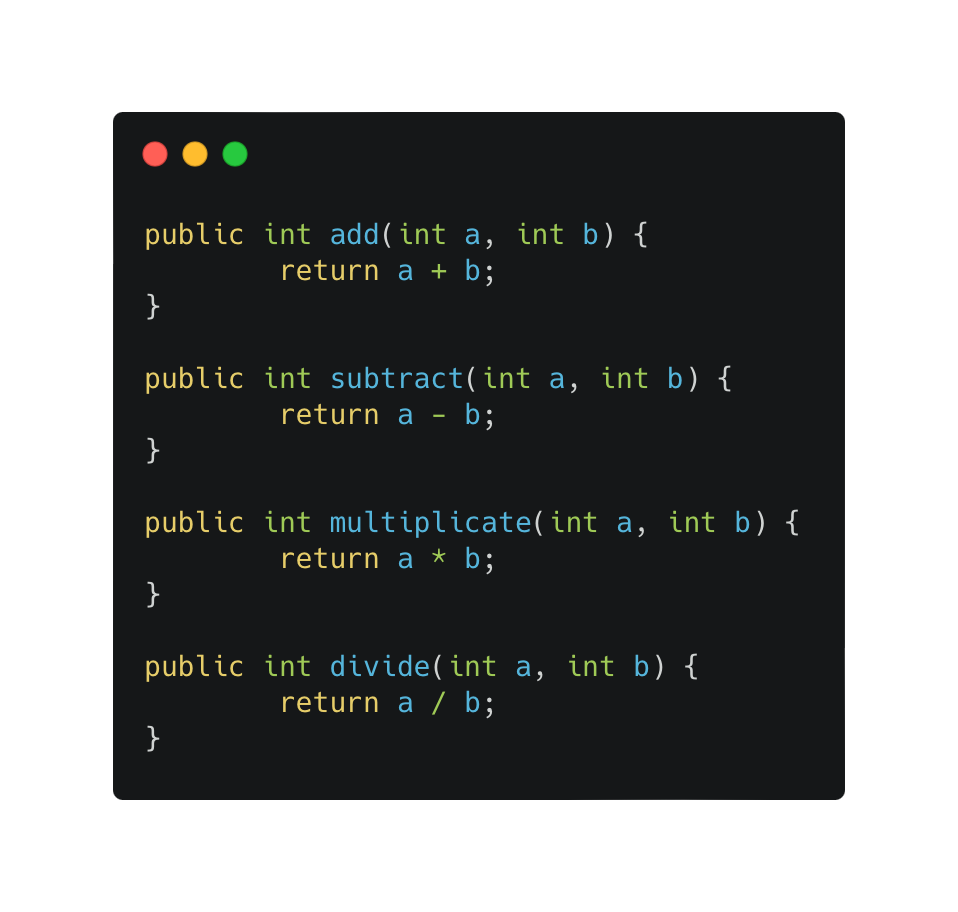
\includegraphics[width=0.6\textwidth]{pic/calc_func.png}
        \centering
        \caption{Ukázkové funkce kalkulačky vhodné pro jednotkové otestování.}
        \label{fig:calc_func}
    \end{figure}

    \begin{figure}[H]
        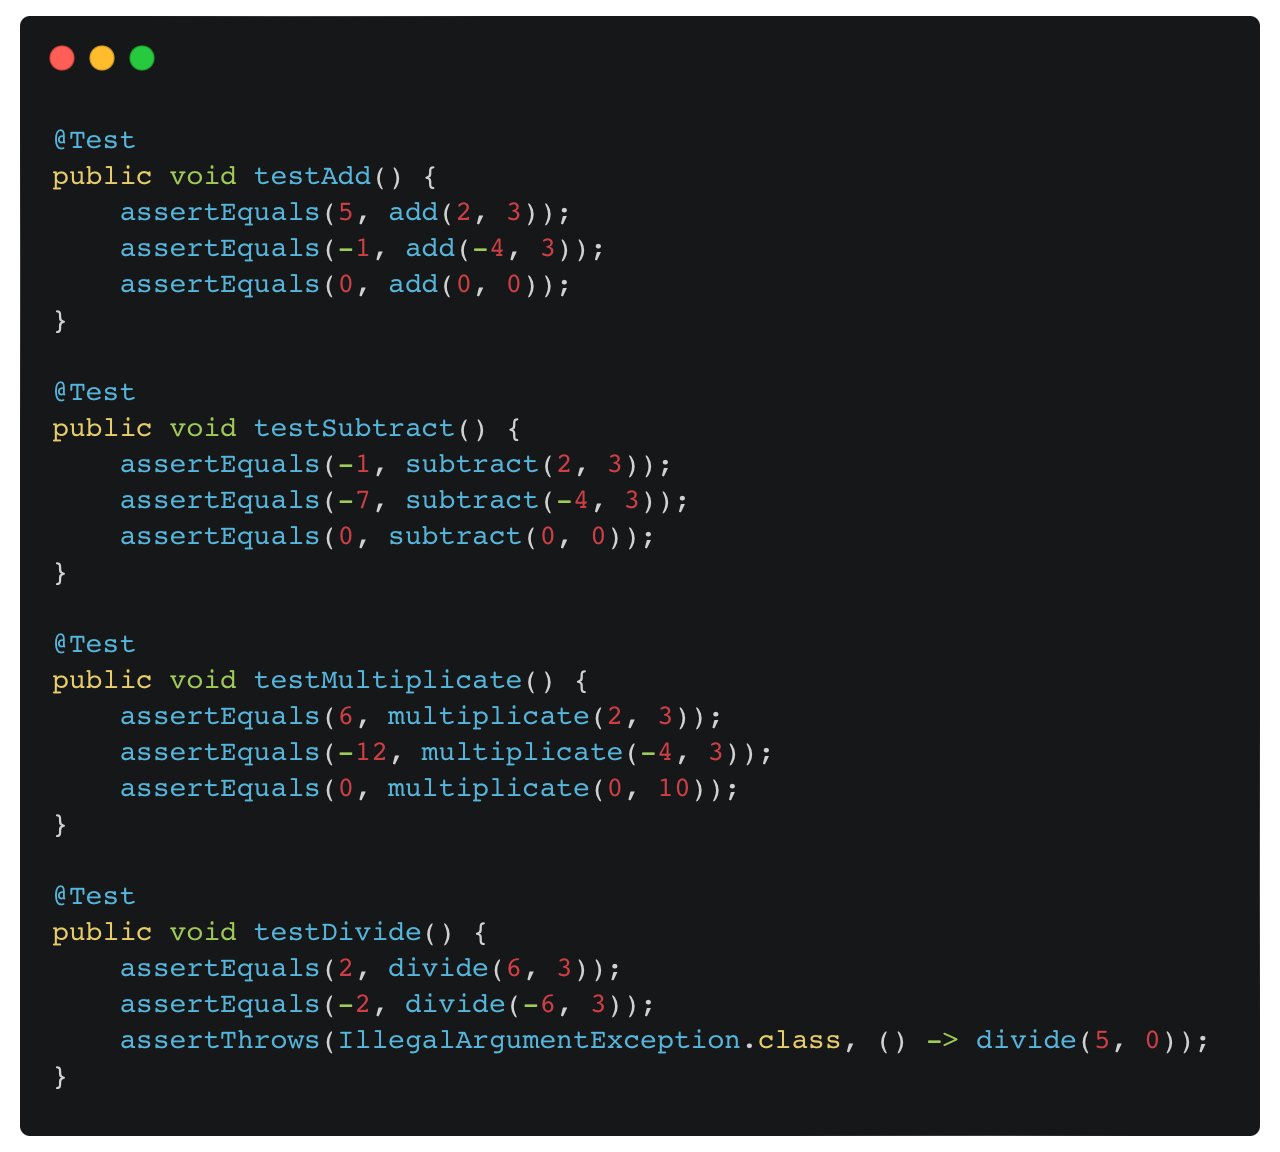
\includegraphics[width=\textwidth]{pic/calc_tests.png}
        \centering
        \caption{Ukázkové jednotkové testy pro funkce kalkulačky.}
        \label{fig:calc_tests}
    \end{figure}

    Testovat je možné nejen zdrojový kód softwaru, ale také jeho grafické rozhraní (dále pouze \Acrshort{gui}). Zde je možné využít stejného manuálního testování jako bylo popsáno výše, ovšem existují i sofistikované automatizované metody. Účelem \Acrshort{gui} testů nemusí být pouze základní ověření funkčnosti na testových scénářích, ale také zajištění, že \Acrshort{gui} se správně chová napřílad na různých zařízeních nebo velikostích obrazovky. Dále lze také ověřovat, zda nové aktualizace neporušili staré funkce (regresní testy) či zhodnotit, zda výkon aplikace odpovídá předpokladu. Tyto testy lze automatizovat jak skriptem (příkladem zde je framework \textit{Robot Framework} nebo \textit{Selenium}, využívané pro testy webu a v tomto projetu) tak skze nástroje umožňující nahrávání uživatelských akcí a interakcí se softwarem a jejich následné přehrání (podobně jako funguje například \textit{makro} v sadě Microsoft Office). Mezi takové nástroje se řadí software jako např. \textit{Ranorex}, \textit{AutoHotKey} či \textit{PyAutoGUI}. \cite{alegroth2016maintenance}

    %TODO Možná metriky, které se u testů sbírají?

    \section{Jazykové modely}

    Velké jazykové modely (zkráceně \Gls{llm}) je druh modelu strojového učení (\Acrshort{ml}), který využívá techniky \textit{hlubokého učení}, které se zaměřují na techniky zpracování a generování přirozeného jazyka (také známé jako techniky \Acrshort{nlp}). Tyto modely jsou navrženy tak, aby rozumněli kontextu a významu jazyka, a dokázali pro \textit{textový vstup} odhadnout (vygenerovat) \textit{textový výstup}. Tato schopnost jim umožňuje provádět široké spektrum operací nad přirozeným jazykem jako sumarizace, překlad textu, generování absahu či dialogu a podobně. Příkladem takových modelů je například známý \textit{GPT} (Generative Pre-trained Transformer) od společnosti OpenAI nebo BERT (Bidirectional Encoder Representations from Transformers).
    \cite{devlin2019bert} \cite{googleML2023} \cite{cloudflareLLM2023}

    \Gls{llm} modely získávají svá data při procesu \textit{trénování}. Jejich trénink zahrnuje analýzu a zpracování obrovského množství textových dat, jejichž řetězce jsou rozděleny na jednotky zvané \gls{token}y. Tokenizace je proces, při kterém je text rozdělen na menší části, které mohou být \textit{slova, části slov} nebo pouze \textit{jednotlivé znaky}. Toto rozdělení Toto rozdělení umožňuje lépe analyzovat a učit se závislosti mezi jednotlivými částmi textu. Každý token je pak převeden na numerický vektor pomocí techniky zvané \emph{embedding}, což jsou vlastně váhy přiřazené jednotlivým tokenům. Váhy v modelu jsou kritické, protože určují, jaký význam a důležitost jednotlivá slova a tokeny mají. Tyto váhy jsou dynamicky upravovány během trénování, aby co nejlépe odráželi vzory a závislosti v tréninkových datech. Model díky těmto hodnotám může model zpracovávat text v matematické formě. Modely jsou většinou předtrénovány na rozsáhlé sadě korpusů textových dat, které zahrnují články, knihy, webové stránky a další prameny obsahující psaný text. Cílem trénování je naučit model základní struktu jazyka bez specifického cíle. Váhy jsou zároveň jedny z parametrů modelu. Dalšími parametry také mohou být zkreslení (bias) jednotlivých vrstev nebo jejich aktivace. Věškteré parametry modelu mohou být upravovány v rámci trénovacího procesu a mají zásadní vliv na výstup modelu. \cite{prazak2022embedding} \cite{prazak2022seq2seq}

    Po natrénování modelu na obecné sadě dat je také možné přejít ke kroku zvanému \uv{fine-tuning}, ve kterém dochází k jeho jemnému doladění, aby jeho schopnosti odpovídali konkrétním úkolům nebo aplikacím, pro které by model měl být použit. K tomu je využita datová sada úzce zaměřená na tuto oblast. Během této fáze se upravují vnitřní parametry modelu tak, aby lépe odpovídali cílovým úkonům. Váhy v modelu, které jsou upravovány, určují, jak model reaguje na různé vstupy během interferenční fáze. Příkladem takového \textit{fine-tuningu} může být úprava modelu pro generování zdrojového kódu specifického programovacího jazyka.

    Pro funkci \Gls{llm} je také důležitý kontext modelu, který je definován jako soubor relevatních informací, které předcházejí nebo následují za aktuálním tokenem a ovlivňují jeho význam nebo použití v dané situlaci. \Gls{llm} využívají kontext k lepšímu porozumění tomu, jak jsou slova používaná ve větách, což umožňuje modelu generovat text, který je koherentní a relevantní k zadaným promptům. Kontext je tedy klíčový pro trénink modelu, protože pomáhá modelu pochopit nejen izolované tokeny, ale také celkovou struktu a význam textu.

    Jazykové modely se spouštějí během procesu zvaného \textit{interference}. Jde o proces, při kterém model generuje výstupy (odpovědi, texty) na základě vstupních dat, které dostává. Těmto vstupním datům se říká \textit{prompt}, kterým je podnět poskytnutý uživatelem jako \textit{otázka, věta k dokončení}, nebo jiný typ zadání, které model používá jako východisko pro generování odpovídajícího textu. Znalosti a kontext nabrané při tréninku jako váhy jsou využity k predikci nejpravděpodobnějších tokenů, které by měli následovat po promptu. Interakce s \Gls{llm} prostřednictvím promptu umožňuje uživatelům specfikovat, jaký typ informace nebo textu chtějí od modelu získat. Modely jsou běžně navrženy tak, aby rozpoznávali struktu jazyka, tak kontext, ve kterém jsou jeho tokeny použity. To umožňuje modelům přizpůsobovat své odpovědi v závislosti na zadání a předchozím textu v konverzaci. \cite{pasekprazak2022}

    \section{Motivace}

    Tím, že tvorba softwarových testů ze specifikací je problém převodu \emph{text na text} (přesněji zdrojový kód), souhlasí tak s funkcí  \Gls{llm}, která spočívá v predikci \emph{textu} na bázi \emph{textového} vstupu (promptu). Jinými slovy jde o stejný problém. Tento předpoklad nám umožňuje převést vytváření testů na automatizovanou činnost s využitím strojového učení. Samotné vytváření testů v softwarovém vývoji je činnost, která je časově náročná a často vyžaduje i zkušeného uživatele (často programátora) pro jejich sestavení. Mimo jejich sestavení je také nutné i manuálně odhadovat chování softwaru, které v rámci speficikace nemusí být dáno. I přes nepopiratelnou důležitosttestů jsou však z výše zmíněných důvodů často neúplné či naprosto opomenuté, což vede k neotestovanému softwaru.

    Naším návrhem tedy je zautomatizovat samotný proces tvorby testů tak, aby je za pomocí jednoduchého nástroje zvládl vytvořit i méně zkušený (neprofesionální) uživatel jako například \textit{tester, manažer, apod}. Potenciálním scénářem může být, když zákazník určí specifikace (případně požadavky či podobně), vývojář vytvoří prototyp softwaru, na kterém poté může tester dle dostupné speficikace definovat chování testu a dle něj je za pomocí automatizovaného procesu sestaven samotná sada testů. Výhodou generování za pomocí \Gls{llm} může být, že mohou do určité míry porozumnět kontextu textu a mohou tak případně odhalit chyby (či stavy), které by nezkušený uživatel nemusel odhadnout. Zároveň jsou oproti člověku rychlé a tím, že jsou naučeny na širokém spektru dat (často čítající programovací jazyky, dokumentace, ...), tak je také možné, že spoustu vzorů ve zdrojových kódech a chování softwaru již viděli v učících datech.

\chapter{Rešerše} \label{sec:research}

    \section{Provedená práce v problematice} \label{sec:previouswork}
        \subsection{Předchozí automatizovaná řešení}
        Jazykové modely nebyli prvními pokusy o automatizované generování jednotkových testů. V sučasnosti existuje spousta metod, které se neustále rozvíjejí a nové vznikají. Mezi ně patří příklady jako \textit{fuzzing, generování náhodných testů řízených zpětnou vazbou, dynamické symbolické vykonání, vyhledávvací a evoluční techniky, parametrické testování}. Zároveň také již na počátku století byly pokusy o vytvoření vlastní neuronové sítě sloužící právě čistě k úkolu testování softwaru (například článek "Using a neural network in the software testing process"). \cite{Vanmali2002UsingAN} V této sekci je ukázka několika z nich. 

        \subsubsection{Programatická řešení}
        Jedna z používaných programatických automatizovaných metod pro tvrobu jednotkových testů je tzv. \textit{fuzzing}. V rámci těchto testů musí uživatel stále definovat jeho kódovou strukturu, resp. akce, které test bude provádět a jaký výstup očekávat. Automaticky generovaný je pouze vstup tohoto testu. Výhodou zde tedy je, že uživatel nemusí vytvářet maketu vstupních dat testu, která se zde vytvoří automatizovaně. Zůstává zde však problematika, že pro uživatele není kód \emph{black-box}, ale celou jeho strukturu včetně požadovaného výstupu musí sám definovat. \cite{fuzzing}

        Pouze vstupy dokáže také generovat metoda \textit{symbolického vykonání}, která postupně analyzuje chování větvení programu. Začíná bez předchozích znalostí a používá řešitel omezení (anglicky označovaný jako \textit{constraint solver}) k nalezení vstupů, které prozkoumají nové vykonávací cesty (anglicky \textit{execution path}) v rámci řízení toku programu. Jakmile jsou testy spuštěny s těmito vstupy, nástroj sleduje cestu, kterou se program ubírá, a aktualizuje svou znalostní bázi \((q)\) s novými podmínkami cesty \((p)\). Tento iterativní proces se opakuje a nadále zpřesňuje sadu známých chování a snaží se maximalizovat pokrytí kódu. \textit{Známé chování} lze definovat jako sadu identifikovaných vykonávacích cest programu, včetně podmínek a stavů, které byly analyzovány a uloženy do znalostní báze nástroje \((q)\). Umožňuje efektivně generovat nové testovací vstupy a předvídat chování programu na základě již známých dat. Nástroje běžně zvládají různé datové typy a respektují pravidla viditelnosti objektů. Snaží se také používat mock objekty a parametrizované makety k simulaci různých chování vstupů, čímž zlepšuje proces generování testů, aby odhalila potenciální chyby a zajistila komplexní pokrytí kódu testy. \cite{parizek_symbolic_execution} Tato metoda je implementována například v nástroji IntelliTest v rámci IDE \textit{Visual Studio}. Je používáná v kombinaci s \emph{parametrickými testy}, také označovanými jako \acrshort{put}. Na rozdíl od tradičních jednotkových testů, které jsou typicky uzavřené a nezměnitelné metody, parametrické testy mohou přijímat libovolné množství parametrů a adaptují se tak testovacím scénářům. Software pro jejich vytváření se pak snaží automaticky generovat (minimální) sadu vstupů, které plně pokryjí kód dosažitelný z testu. Nástroje jako např. \textit{IntelliTest} automaticky generují vstupy pro \acrshort{put}, které pokrývají mnoho vykonávacích cest testovaného kódu. Každý vstup, který pokrývá jinou cestu, je "serializován" jako jednotkový test. Parametrické testy mohou být také generické metody (funkce schopná pracovat s různými druhy datových typů bez nutnosti psát pro každý typ specifický kód zvlášť), v tom případě musí uživatel specifikovat typy použité k instanci metody. Testy také mohou obsahovat atributy pro \emph{očekávané} (např. dělení nulou) a případně \emph{neočekávané} vyjímky (např. předání reference na nulový objekt). Neočekávané vyjímky vedou k selhání testu. \acrshort{put} tedy do velké míry redukují potřebu uživatelského vstupu pro tvorbu jednotkových testů. \cite{IntelliTestInputGeneration2023} \cite{microsoft2023testgen}

        Pokud zvolíme symbolické řešení vstupu (některé vstupní argumenty testovaného programu nebudou reprezentovány konktrétními hodnotami, ale zastoupené symbolickými proměnnými) společně s determinovanými vstupy (využity konkrétní hodnoty) a vykonávací cestou, vzniká tak hybridní řešení zvané jako \emph{konkolické testovaní} nebo \emph{dynamické symbolické vykonání}. Tento druh testů dokáží tvořit nástroje jako \textit{SAGE, KLEE} nebo \textit{S2E}. Problémem tohoto přístupu však je, když program vykazuje \emph{nedeterministické} chování, kdy tyto metody nebudou schopny určit správnou cestu a zároveň tak ani zaručit dobré pokrytí kódu/větví. Nedeterministické chování není tolik obvyklé a objevuje se zejména v případě \textit{paralelizmu}, \textit{externího přerušení} či u algortimů postavených na \textit{pseudonáhodě}. \cite{ncatlab_nondeterministic_computation} Tento problém není speficický pouze pro tento typ automatizovaného testování, ale i pro předchozí varianty. Zatímco \emph{symbolická} část vykonání objeví veškeré možné cesty, \emph{konkrétní} vykonání poté určí sled jednotlivých událostí při spuštění, aby nedocházelo k redundantnímu testování. \cite{aldrich2019concolic} Dalším problémem této metody také může být výběr stavových proměnných. Problémem je zejména jejich rozsah. Například více stavových proměnných s malým celočísleným rozsahem povede pouze k omezenému množství cest, kdežto pouze jednotky takových proměnných o celém rozsahu typu \verb|double| může vést k daleko vyššímu počtu cest, což také zvýší výpočetní náročnost těchto metod a tedy se i snižuje pravděpodobnost úspěšného nenalezení praktického řešení (v případě, že takové řešení vůbec existuje nebo je to účelem vyhledávání). \cite{concolic_chalenges_2019} \cite{engler2006exe} \cite{sen2005cute} \cite{zhou2006safedrive}

        Další metodou je \textit{náhodné generování testů řízené zpětnou vazbou}, která je vylepšením pro generování náhodných testů tím, že zahrnuje zpětnou vazbu získanou z provádění testovacích vstupů v průběhu jejich vytváření. Tato technika postupně buduje vstupy tím, že náhodně vybírá metodu volání (jedná se o dostupnou funkci nebo metodu v rámci programu) a hledá hodnoty argumentů, které náhodně generuje nebo upravuje vstupy vytvořenými v předchozích iteracích tohoto procesu. Jakmile dojde k sestavení vstupu, je provedeno jeho vykonání a výsledek ověřen proti sadě \gls{kontrakt}ů a \glspl{filtr}ů. Výsledek vykonání jeho srovnáním s očekávanými výstupy, definovanými v kontraktu, a filtry určuje, zda je vstup redundantní (definován tak filtry), proti pravidlům (jak filtrů tak kontraktů), porušující \gls{kontrakt} (např. nedefinované výstupy) nebo užitečný pro generování dalších vstupů (splňuje konktrakt a prochází filtry). Technika vytváří sadu testů, které se skládají z jednotkových testů pro testované třídy. Úspěšné testy mohou být použity k zajištění faktu, že \glspl{kontrakt} kódu jsou zachovány napříč změnami programu; selhávající testy (porušující jeden nebo více kontraktů) ukazují na potenciální chyby, které by měly být opraveny. Tato metoda dokáže vytvořit nejen vstup pro test, ale i tělo (kód) testu. Ovšem pro uživatele je stále vhodné znát strukturu kódu. \cite{FeedbackDirectedRT}

        Z programatických metod se zdají být nejpokročilejší \emph{evoluční algoritmy} pro generování sad jednotkových testů, využívající přístup založený na vhodnosti (fitness funkce), aby vyvíjely testovací případy, které mají za cíl maximalizovat pokrytí kódu a detekci chyb. Na rozdíl od náhodného generování, které vytváří testy bez specifického cíle, evoluční algoritmy používají fitness funkci k iterativnímu zdokonalování testů na základě jejich schopnosti odhalovat chyby a efektivně prozkoumávat kód. Tyto algoritmy mohou autonomně generovat testovací vstupy, které jsou navrženy tak, aby prozkoumávaly různé vykonávací cesty v aplikaci a dynamicky se upravují na základě pozorovaných výsledků, což zvyšuje jejich účinnost a snižuje potřebu manuálního vstupu. Uživatelé mohou interagovat s vygenerovanými testy jakožto s \textit{black-boxem}. Testy se zaměřují na vstupy a výstupy, aniž by potřebovali rozumět vnitřní logice testovaného systému. Tento aspekt evolučního testování je zvláště výhodný při práci se složitými systémy nebo když zdrojový kód není snadno dostupný. Proces iterativně upravuje testovací případy na základě pozorovaných chování, upravuje vstupy pro efektivnější prozkoumání systému a identifikaci potenciálních defektů. Tato metoda podporuje vysokou úroveň automatizace při generování testů, snižuje potřebu manuálního vstupu a umožňuje komplexní pokrytí testů s menším úsilím. \cite{CAMPOS2018207} \cite{abs-2111-05003}

        \subsubsection{Neuronové sítě}
        Ke generování jednotkových testů lze využít i vlastní neuronové sítě. Takové se pokoušeli vytvářet například v práci "Unit test generation using machine learning"\cite{Saes2018UnitTestGeneration}, kde byly testovány primárně \Acrshort{rnn} a experimentálně \Acrshort{cnn} sítě (ty však měli problém s větším množstvím tokenů). Modely byli testovány na programech napsaných v jazyce Java. Metoda se zaměřila na programy s plným přístupem k jejich zdrojovému kódu a zkompilovanému bytkódu, což umožnilo detailní analýzu z pohledu white box. Při nejlepší konfiguraci dosáhl výsledek modelu \(70.5\%\) parsovatelného kódu (tedy takového bez chyb, který lze spustit) natrénovaný z bezmála 10000 příkladů \textit{zdrojový kód - test}. Výsledek práce je však stále jakýsi "proof of concept", protože zatímco vygenerují částečně použitelný výsledek, je vždy nutný zásah experta, aby mohlo dojít k vytvoření celého testovacího souboru. Takovéto sítě se však mohou silně hodit jako výpomoc programátorovi při psaní testů.

        \subsubsection{Nevýhody současných metod}
        Současné metody generování jednotkových testů, jako je \textit{fuzzing} a \textit{symbolické vykonání}, často vyžadují podrobnou znalost struktury kódu a očekávaných výstupů, což omezuje jejich efektivitu a zvyšuje složitost tvorby testů. Jen některé z těchto metod jsou schopné vygenerovat testy pouze na bázi specifikace (z black box pohledu) bez vnitřní znaloasti kódu. Většina z klasických metod je zároveň schopna generovat pouze vstupy jednotkových testů, ale už ne samotné tělo (kód) testu nebo očekávané výstupy, a tedy pouze složí jako jakási konstra pro programátora, který musí test doimplementovat.

        Velké jazykové modely (\gls{llm}) mohou být atraktivní alternativou, protože pomocí nich lze potenciálně automatizovat generování jak vstupů pro testy, tak přidruženého testovacího kódu, čímž se snižuje potřeba hlubokého porozumění struktuře kódu. S takovým nástrojem není potřeba programátora, ale může s ním pracovat i méně zkušený uživatel (např. \textit{tester}). Dále je zde možnost otestovat kód za pomocí slovní specifikace pro funkci nebo vlastnosti. Takové specifikace se používají napřílad v \textit{aero-space} nebo \textit{automotive} sektoru. \cite{KuglerMaag2024SysReqAnalysis} \GLS{llm} také mohou objevit jiné možné stavy, které mohou u vstupu nebo výstupu nastat a pokusit se pro ně navrhnout test, případně nedokonalosti ve specifikaci, které mohou obejít.

    \subsection{Vydané publikace}
    Jeden z poměrně nedávno vydaných článků (září 2023) nazvaný "An Empirical Evaluation of Using Large Language Models for Automated Unit Test Generation" \cite{schafer2023empirical} se zabývá využitím velkých jazykových modelů (\gls{llm}) pro automatizované generování jednotkových testů v jazyce JavaScript. Implementovali nástroj s názvem \textbf{TESTPILOT}, který využívá \gls{llm} \textit{gpt3.5-turbo}, \textit{code-cushman-002} od společnosti OpenAI a  také model StarCoder, který vznikl jako komunitní projekt \cite{StarCoder2023}. Vstupní sada pro \gls{llm} obsahovala signatury funkcí, komentáře k dokumentaci a příklady použití. Nástroj byl vyhodnocen na 25 balíčcích npm obsahujících celkem 1684 funkcí API. Vygenerované testy dosáhly pomocí gpt3.5-turbo mediánu pokrytí příkazů 70,2\% a pokrytí větví 52,8\%, čímž překonaly nejmodernější techniku generování testů v jazyce JavaScript zaměřenou na zpětnou vazbu, Nessie.

    Zmíněný model \emph{StarCoder} byl představen v článku "StarCoder: may the source be with you!" \cite{StarCoder2023} z května 2023. Vytvořeny byly konkrétně 2 verze, \textit{StarCoder} a \textit{StarCoderBase}, s 15,5 miliardami parametrů a délkou kontextu 8K. Tyto modely jsou natrénovány na datové sadě nazvané \textit{The Stack}, která obsahuje 1 bilion tokenů z permisivně licencovaných repozitářů GitHub. \textit{StarCoderBase} je vícejazyčný model, který překonává ostatní modely open-source \gls{llm} modely, zatímco \textit{StarCoder} je vyladěná verze speciálně pro Python, která se vyrovná nebo překoná stávající modely zaměřené čistě na Python. Článek poskytuje komplexní hodnocení, které ukazuje, že tyto modely jsou vysoce efektivní v různých úlohách souvisejících s kódem.

    Článek "Exploring the Effectiveness of Large Language Models in Generating Unit Tests" \cite{siddiq2023exploring} z dubna 2023 hodnotí výkonnost tří \gls{llm} - \textit{Codex}, \textit{CodeGen} a \textit{GPT-3.5} - při generování jednotkových testů pro třídy jazyka Java. Studie používá jako vstupní sady dva benchmarky, \href{https://paperswithcode.com/dataset/humaneval-x}{HumanEval}\footnote{\url{https://ai.google.dev/gemma/terms}} a \href{https://paperswithcode.com/dataset/evosuite-sf110-benchmark}{Evosuite SF110}\footnote{\url{https://paperswithcode.com/dataset/evosuite-sf110-benchmark}}. Klíčová zjištění ukazují, že \textit{Codex} dosáhl více než 80\% pokrytí v datové sadě \textit{HumanEval}, ale žádný z modelů nedosáhl více než 2\% pokrytí v benchmarku \textit{SF110}. Kromě toho se ve vygenerovaných testech často objevovaly tzv. \gls{testsmells}, jako jsou \textit{duplicitní tvrzení} a \textit{prázdné testy} \cite{testsmells}.

    \subsubsection{Srovnání výsledků}
    Výsledky diskutovaných studií v předchozím bodě jsme srovnali v tabulce \ref{tab:paper_comp}. V rámci první práce dosahuje nejlepších výsledků model \textit{gpt-3.5-turbo}, který dosáhl 70\% pokrytí kódu testy a 48\% úspěšnosti testů. U druhé studie má tento model na testovací sadě \textit{HumanEval} velice podobný výsledek, ovšem model \textit{Codex} dosáhl lepších výsledků. Může však také jít o rozdíl způsobený programovacím jazykem. Zatímco v práci \cite{schafer2023empirical} se využívá jako benchmark sada balíčků v jazyce \textit{JavaScript}, který kvůli absenci explicitního typování, může být obtížnější pro strojové testování oproti jazyku Java, který je využit ve zbylých 2 pracích. \cite{jutai} také využívá Javu a s modelem \textit{gpt-3.5-turbo} dosahuje podobného pokrytí kódu a úspěšnosti jako \textit{Codex} v práci \cite{siddiq2023exploring}.


    \subsection{Modely} \label{sec:research_models}
    Na \GLS{llm} modelech nás konkrétně zajímá schopnost pozorumět progamovacím jazykům a ty poté také generovat na výstupu. Důležité pro nás také je, zda daný model je proprietární či otevřený a pod jakou licencí, tedy zda by byl vhodný pro naši práci. V případě analýzy zdrojového kódu může být také klíčovou vlastností délka kontextu daného modelu. Tyto vlastnosti jsou také zaneseny do tabulky \ref{tab:code_models_comp}.

    \paragraph{StarCoder} Jedním z často používaných modelů v předchozích pracích \cite{schafer2023empirical} je \textit{StarCoder} a \textit{StarCoderBase}, diskutovaný již v sekci \ref{sec:previouswork}. \textit{Base} verze je schopna generovat kód pro více jak 80 programovacích jazyků. Model je navržen pro širokou škálu aplikací obsahující \textit{generování}, \textit{modifikaci}, \textit{doplňování} a \textit{vysvětlování} kódu. Jeho distribuce je volná a licence \textbf{CodeML OpenRAIL-M 0.1} \cite{BigCode2023} umožňuje ho využívat pro množštví aplikací včetně komerčních nebo edukačních. Jeho uživatel však má povinnost uvádět, že výsledný kód byl vygenerován modelem. Licence má své restrikce z obavy tvůrců, protože by model mohl někoho při nepsrávném použití ohrozit. Tyto restrikce se aplikují na na všechny derivace projektů pod touto licencí. Zároveň není kompatibilní s Open-Source licencí právě kvůli těmto restrikcím.

    Model StarCoder se také dočkal novější verze \textit{StarCoder2}, který nepřímo navazuje na model \textit{StarCoderBase}. Je naučen na archivu GitHub repoziářů archivovaných v rámci organizace \textit{Software Heritage}, čítajících přes 600 programovacích jazyků a dalších pečlivě vybraných dat jako například \textit{pull requesty}. Mimo toho také trénovací data obsahují staženou dokumentaci k vybraným projektům. Model se vyjímá tím, že se snaží udržet malou velikost. Je nabízen ve verzích s \textit{3, 7} a \textit{15} miliardy parametrů, i přesto však dle jejich úvodní studie \cite{lozhkov2024starcoder} nabízí na sadě populárních programovacích jazyků shodné či lepší výsledky oproti modelu \textit{CodeLlama} s 34 miliardy parametrů. Výhodou tohoto modelu nepochybně je, že ho lze spustit na spoustě dnešních počítačů s plným offloaded na grafickou kartu.

    \paragraph{CodeLlama} Nedávno vydaným modelem je \textit{Code Llama} od společnosti Meta. Jedná se o evoluci jejich jazykového modelu \textit{Llama} specializovaný však čistě na úlohy kódování. Je postaven na platformě \textit{Llama 2} a existuje ve třech variantách: \textit{základní Code Llama}, \textit{Code Llama - Python} a \textit{Code Llama - Instruct}. Model podporuje více programovacích jazyků, včetně jazyků jako Python, C++, Java, PHP, Typescript, C# nebo Bash. Je určen pro úlohy, jako je generování kódu, doplňování kódu a ladění. Code Llama je zdarma pro výzkumné i komerční použití a je uvolněn pod licencí MIT. Uživatelé však musí dodržovat  zásady přijatelného použití, ve kterých je uvedeno, že model nelze použít k vytvoření služby, která by konkurovala vlastním službám společnosti Meta. \cite{roziere2024code} I samotný model \textit{LLama 2}, případně novější verze \textit{LLama 3} by měli být schopné generovat zdrojový kód a oproti \textit{CodeLlama} modelu mohou mít v některých ohledech lepší predikci pro tokeny v obecném kontextu. \cite{metallama3introduction}

    \paragraph{Copilot} Velmi populárním nástrojem pro generování kódu za pomocí \gls{llm} je \href{https://github.com/features/copilot}{GitHub Copilot}\footnote{\url{https://github.com/features/copilot}}, který je postaven na modelu \textit{codex} od OpenAI. Původní model však byl přestal být zákazníkům nabízen a namísto něj OpenAI doporučuje ke generování kódu využívat chat verze modelů GPT-3.5 a GPT-4. Na architektuře GPT-4 je také postavený nástupce služby Copilot, \href{https://github.com/features/preview/copilot-x}{Copilot X}\footnote{\url{https://github.com/features/preview/copilot-x}}. Zmíněné modely chat GPT-3.5 a GPT-4 jsou primárně určeny pro generování textu formou chatu. Zvládají však zároveň i dobře generovat kód a jsou vhodné i úlohu generování jednotkových testů. \cite{openai2024gpt4} Narozdíl od předchozích modelů však nejsou volně distribuovány a jsou poskytovány pouze jako služba společností OpenAI skrze API nebo je lze hostovat v rámci služby Azure společnosti Microsoft, která zajišťuje větší integritu dat. Jedná se tedy o uzavřený model a jeho uživatelé musí souhlasit s jeho podmínkami použití.

    \paragraph{Anthropic} Velmi schopným modelem, který jak jeho tvůrci\footnote{\url{https://www.anthropic.com/news/claude-3-family}} tak i nezávislé strany pusuzují jakožto stejně přesný a inteligentní, ne-li v některých případech přesnější a schopnější jak model GPT-4, je Claude 3 od společnosti Anthropic. \cite{kevian2024capabilities} Ten je nabízen ve 3 varintách: \textit{Opus, Sonnet a Haiku}, kdy verze \textit{Opus} je s počtem 137 miliard parametrů a kontextovým oknem 200 tisíc tokenů největší z nich a ostatní využívají méně parametrů. Znamená to ale také, že mají nižší cenu, protože rodina modelů Claude 3 je pouze proprietární a dostupná buďto skrze API společnosti Anthropic či na službě AWS. Mimo EU je také dostupný v rámci chatovací aplikace. \cite{anthropic2023claude}

    \paragraph{Cohere} Podobně jako společnost Meta, vydává otevřené modely i startup \textit{Cohere}, který stojí za modely jako \textit{Command, Command R a Command R+}. Většina z nich je otevřena\footnote{Např. model Command R+: \url{https://huggingface.co/CohereForAI/c4ai-command-r-plus}} pro \emph{nekomerční} použití (pod licencí CC-BY-NC-4.0) a tedy volně použitelné např. pro výzkumné a neziskové účely. Mimo základních schopností tyto modely oficiálně podporují více jak 13 mluvených jazyků. Zároveň modely \textit{Command R(+)} byli navrženy se schopností využívat zdrojování metodou \Gls{rag} za pomocí konektorů, kterými může být například \textit{internetový vyhledávač} nebo \textit{lokální soubory}. Sám tvůrce však upozorňuje na fakt, že větší modely jsou vhodné spíše pro účely \Acrshort{ir}, zatímco pro běžné úlohy sumarizace je vhodný menší a proprietární model \textit{Command}. I přes fakt, že tyto modely lze provozovat \textit{lokálně}, je zde problém ve velké náročnosti na hardware. Modely jsou však dostupné i skze nejen oficiální API, ale i jako služba u cloudových poskytovatelů. \cite{cohere_models} \cite{ruder_command_r}

    \paragraph{Google} Společnost Google v současnosti nabízí 2 rodiny LLM modelů a to víceúčelové \textit{Gemini}\footnote{\url{https://deepmind.google/technologies/gemini/}}, které jsou proprietární a dostupné ve verzi 1.0 Pro a Ultra a novější 1.5 Pro. Google také vypustil malé modely pro generování zdrojového kódu s názvem \textit{Gemma} a pod upravenou Apache 2.0 licencí\footnote{\url{https://ai.google.dev/gemma/terms}}. Podobně jako \textit{Command R} modely mají schopnost podkládat svůj výstup na bázi webového vyhledání nebo poskytnutých dokumentů. V případě modelu \textit{Gemini 1.5 Pro} je tato schopnost navíc rozšířena tím, že podporuje kontext s velikostí až 1 milion tokenů. Tato schopnost může přijít vhod například pro návrh zdrojového kódu v rámci větší kódové základny. Gemini je dostupné v základním modelu 1.O Pro zdarma (dříve Bard), ovšem služba Gemini Studio nabízející ostatní modely není v současnosti dostupná v EU a tedy jediný přístup k modelům je skrze API v rámci služby Google Cloud\footnote{https://cloud.google.com/vertex-ai}.

    Rodina modelů Gemma je poté volně dostupná a to v provedení se 2 nebo 7 miliardy tokenů a ve verzích \textit{Base} a \textit{Instruct}. Dle tvůrců by model měl být pro účely psaní zdrojového kódu, matematického zápisu a logiky přesnější jak model \textit{Llama 2} ve verzi se 13 miliardy paramterů. \cite{gemma_introduction} V rámci upravené licence se společnost \textit{Google} vzdává odpovědnosti za kôd vygenerovaný těmito modely.

    \paragraph{Mistral} Open-source modely schopné generovat kód také nabízí společnost Mistral společně s jejich proprietárními modely jako \textit{Mistral Large} modelem. Jedním z jejich prvních otevřeně vydaných modelů byl \textit{Mistral 7B}, který jak název vypovídá obshuje pouze 7 miliard parametrů, ale i přes tento fakt je schopen v některých katergoriích překonat větší modely jako například \textit{Llama 2}. \cite{jiang2023mistral} Výhodou je, že může být jednoduše vyladěn pro potřeby specifické aplikace. Jejich dalším modelem je také \textit{Mixtral 8x7B} cílící na dosažení stejných kvalit jako např. model \textit{GPT-3.5 Turbo} v běžně používaných benchmarcích. Jeho větší varianta \textit{Mistral 8x22B} pak přidává podporu pro další mluvené jazyky. \cite{jiang2024mixtral} Všechny jejich otevřené modely jsou uvolněny pod licencí Apache 2.0. Mezi jejich proprietární modely se pak řadí model \textit{Mistral Small} a zejména \textit{Mistral Large}\footnote{\url{https://mistral.ai/news/mistral-large/}}, který podobně jako \textit{Mistral 8x22B} zvládá více jazyků tak i podporuje \Gls{rag}. Dostupný je jako API na jejich vlastní platformě \textit{Le Platforme} či u cloudových poskytovatelů.

        \newpage

        \begin{landscape}
            \vspace*{\fill}
            \begin{table}[H]
                \begin{tabular}{|p{6cm}|c|c|c|c|}
                    \hline
                    \textbf{Práce} & \textbf{Model} & \textbf{Benchmark} & \textbf{Pokrytí testy} & \textbf{Úspěšnost} \\
                    \hline
                    \multirow{3}{6cm}{An Empirical Evaluation of Using Large Language Models for Automated Unit Test Generation} & \textit{gpt-3.5-turbo} & \multirow{3}{*}{Sada NPM balíčků} & 70.2\% & 48\% \\
                     & \textit{code-cushman-002} & & 68.2\% & 47.1\% \\
                     & \textit{StarCoder} & & 54\% & 31.5\% \\
                    \hline
                    \multirow{6}{6cm}{Exploring the Effectiveness of Large Language
Models in Generating Unit Tests} & \multirow{2}{*}{\textit{gpt-3.5-turbo}} & HumanEval & 69.1\% & 52.3\% \\
                     & & SF110 & 0.1\% & 6.9\% \\
                     & \multirow{2}{*}{\textit{CodeGen}} & HumanEval & 58.2\% & 23.9\% \\
                     & & SF110 & 0.5\% & 30.2\% \\
                     & \multirow{2}{*}{\textit{Codex (4k)}} & HumanEval & 87.7\% & 76.7\% \\
                     & & SF110 & 1.8\% & 41.1\% \\
                    \hline
                    Java Unit Testing with AI: An AI-Driven Prototype for Unit Test Generation & \textit{gpt-3.5-turbo} & JUTAI - Zero-shot, temperature: \(0\) & 84.7\% & 71\% \\
                    \hline
                \end{tabular}
                \centering
                \caption{Přehled a srovnání studií}
                \label{tab:paper_comp}
            \end{table}
            \vspace*{\fill}

            \pagebreak

            \vspace*{\fill}
            \begin{table}[H]
                \begin{tabular}{|c|c|c|c|c|c|}
                    \hline
                    \textbf{Model} & \textbf{Otevřenost} & \textbf{Licence} & \textbf{Počet parametrů} & \textbf{Programovacích jazyků} & \textbf{Datum vydání} \\
                    \hline
                    \textit{StarCoderBase} & Volně dostupný & CodeML OpenRAIL-M 0.1 & 15.5 miliardy & 80+ & 5/2023 \\
                    \hline
                    \textit{CodeLlama} & Volně dostupný & Llama 2 Licence & 34 miliard & 8+ & 8/2023 \\
                    \hline
                    \textit{gpt-3.5-turbo} & Uzavřený & Proprietární & 175 miliard? & ? & 5/2023 \\
                    \hline
                    \textit{gpt-4} & Uzavřený & Proprietární & 1.76 bilionu & ? & 3/2023 \\
                    \hline
                    \textit{claude-3-opus} & Uzavřený & Proprietární & 137 miliard & ? & 3/2024 \\
                    \hline
                    \textit{command} & Uzavřený & Proprietární & 52 miliard & ? & ? \\
                    \hline
                    \textit{command-r} & Volně dostupný & CC-BY-NC-4 & 35 miliard & ? & 3/2024 \\
                    \hline
                    \textit{command-r-plus} & Volně dostupný & CC-BY-NC-4 & 104 miliard & ? & 4/2024 \\
                    \hline
                    \textit{mistral-7b} & Volně dostupný & Apache 2.0 & 7 miliard & ? & 9/2023 \\
                    \hline
                    \textit{mixtral-8x7b} & Volně dostupný & Apache 2.0 & 7 miliard & ? & 2/2024 \\
                    \hline
                    \textit{mixtral-8x22b} & Volně dostupný & Apache 2.0 & 22 miliard & ? & 4/2024 \\
                    \hline
                    \textit{mixtral-large} & Uzavřený & Proprietární & ? & ? & 2/2024 \\
                    \hline
                    \textit{gemma} & Volně dostupný & Gemma & 7 miliard & ? & 2/2024 \\
                    \hline
                \end{tabular}
                \centering
                \caption{Přehled a srovnání modelů generujících kód}
                \label{tab:code_models_comp}
            \end{table} 
            \vspace*{\fill}
        \end{landscape}
    
    \section{Testovací program} \label{sec:test_program}

    Pro účely této práce jsme se rozhodli vydat cestou \acrshort{gui} testů, konkrétně webových stránek / webové aplikace. Mezi požadavky na testovanou aplikaci a její výběr bylo mimo možnosti vytvořit pro ní automatiovanou sadu testů, také možnost zavedení (\emph{injekce}) chyb do aplikace, díky kterým bude možno ověřit nejen fakt, že vygenerované testy jsou schopné detekovat \textit{korektní} chování softwaru, ale také úspěšně detekovat \textit{chyby}. Volitelnou podmínkou také byla existence již existujících testů vytvořených lidským programátorem, se kterými by bylo možné strojově generované testy porovnat.
    
    Těmto požadavkům vyhovuje jeden z předešlých univerzitních projektů nazvaný \textbf{TbUIS} (\textit{Testbed University Information System}), na který vytvořili Matyáš a Šmaus pod vedením doc. Herouta. \cite{Matyas2018} \cite{Smaus2019} Aplikace představuje \textit{maketu} univerzitního informačního systému, avšak i tak implementuje většinu functionality, kterou bysme od podobného systému čekali a nabízí pohled jak ze strany \textit{studenta} tak ze strany \textit{vyučujícího} (viz obr. \ref{fig:tbuis}). Funkce tohoto systému vycházejí ze sady \textit{use casů}, které popisuje web \footnote{Aplikaci lze nalézt na adrese: \url{https://projects.kiv.zcu.cz/tbuis/web/}} aplikace. Výhodou tohoto systému primárně je, že nabízí nejen plně funkční a otestovanou variantu, ale také \(27\) dalších poruchových klonů, vždy porušující alespoň jeden \textit{use case} a s ním potenciálně spojený test.

    Projekt dále také obsahuje i sadu jak \textit{funkčních} testů primárně pro backend vytvořených Poubovou tak také \textit{akceptačních} testů držejících se pevně specifikací, vytvořených Vaisem. \cite{Poubova2019} \cite{Vais2020} Tyto testy využívají nejen pevné znalosti jednotlivých uživatelských scénářů, ale také jsou parametrizovány pomocí všech dostupných dat k aplikaci (\textit{např. uživatelská jména, předměty, zkoušky, atd.}) k vyhodnocení chování softwaru v co nejvíce případech. Právě \textit{akceptační} testy využívají námi zvolený \textbf{RobotFramework} pro testování a tedy vytvořené scénáře bude možné do určité míry přirovnat a případně zhodnotit jejich kvalitu. 

    \begin{figure}
        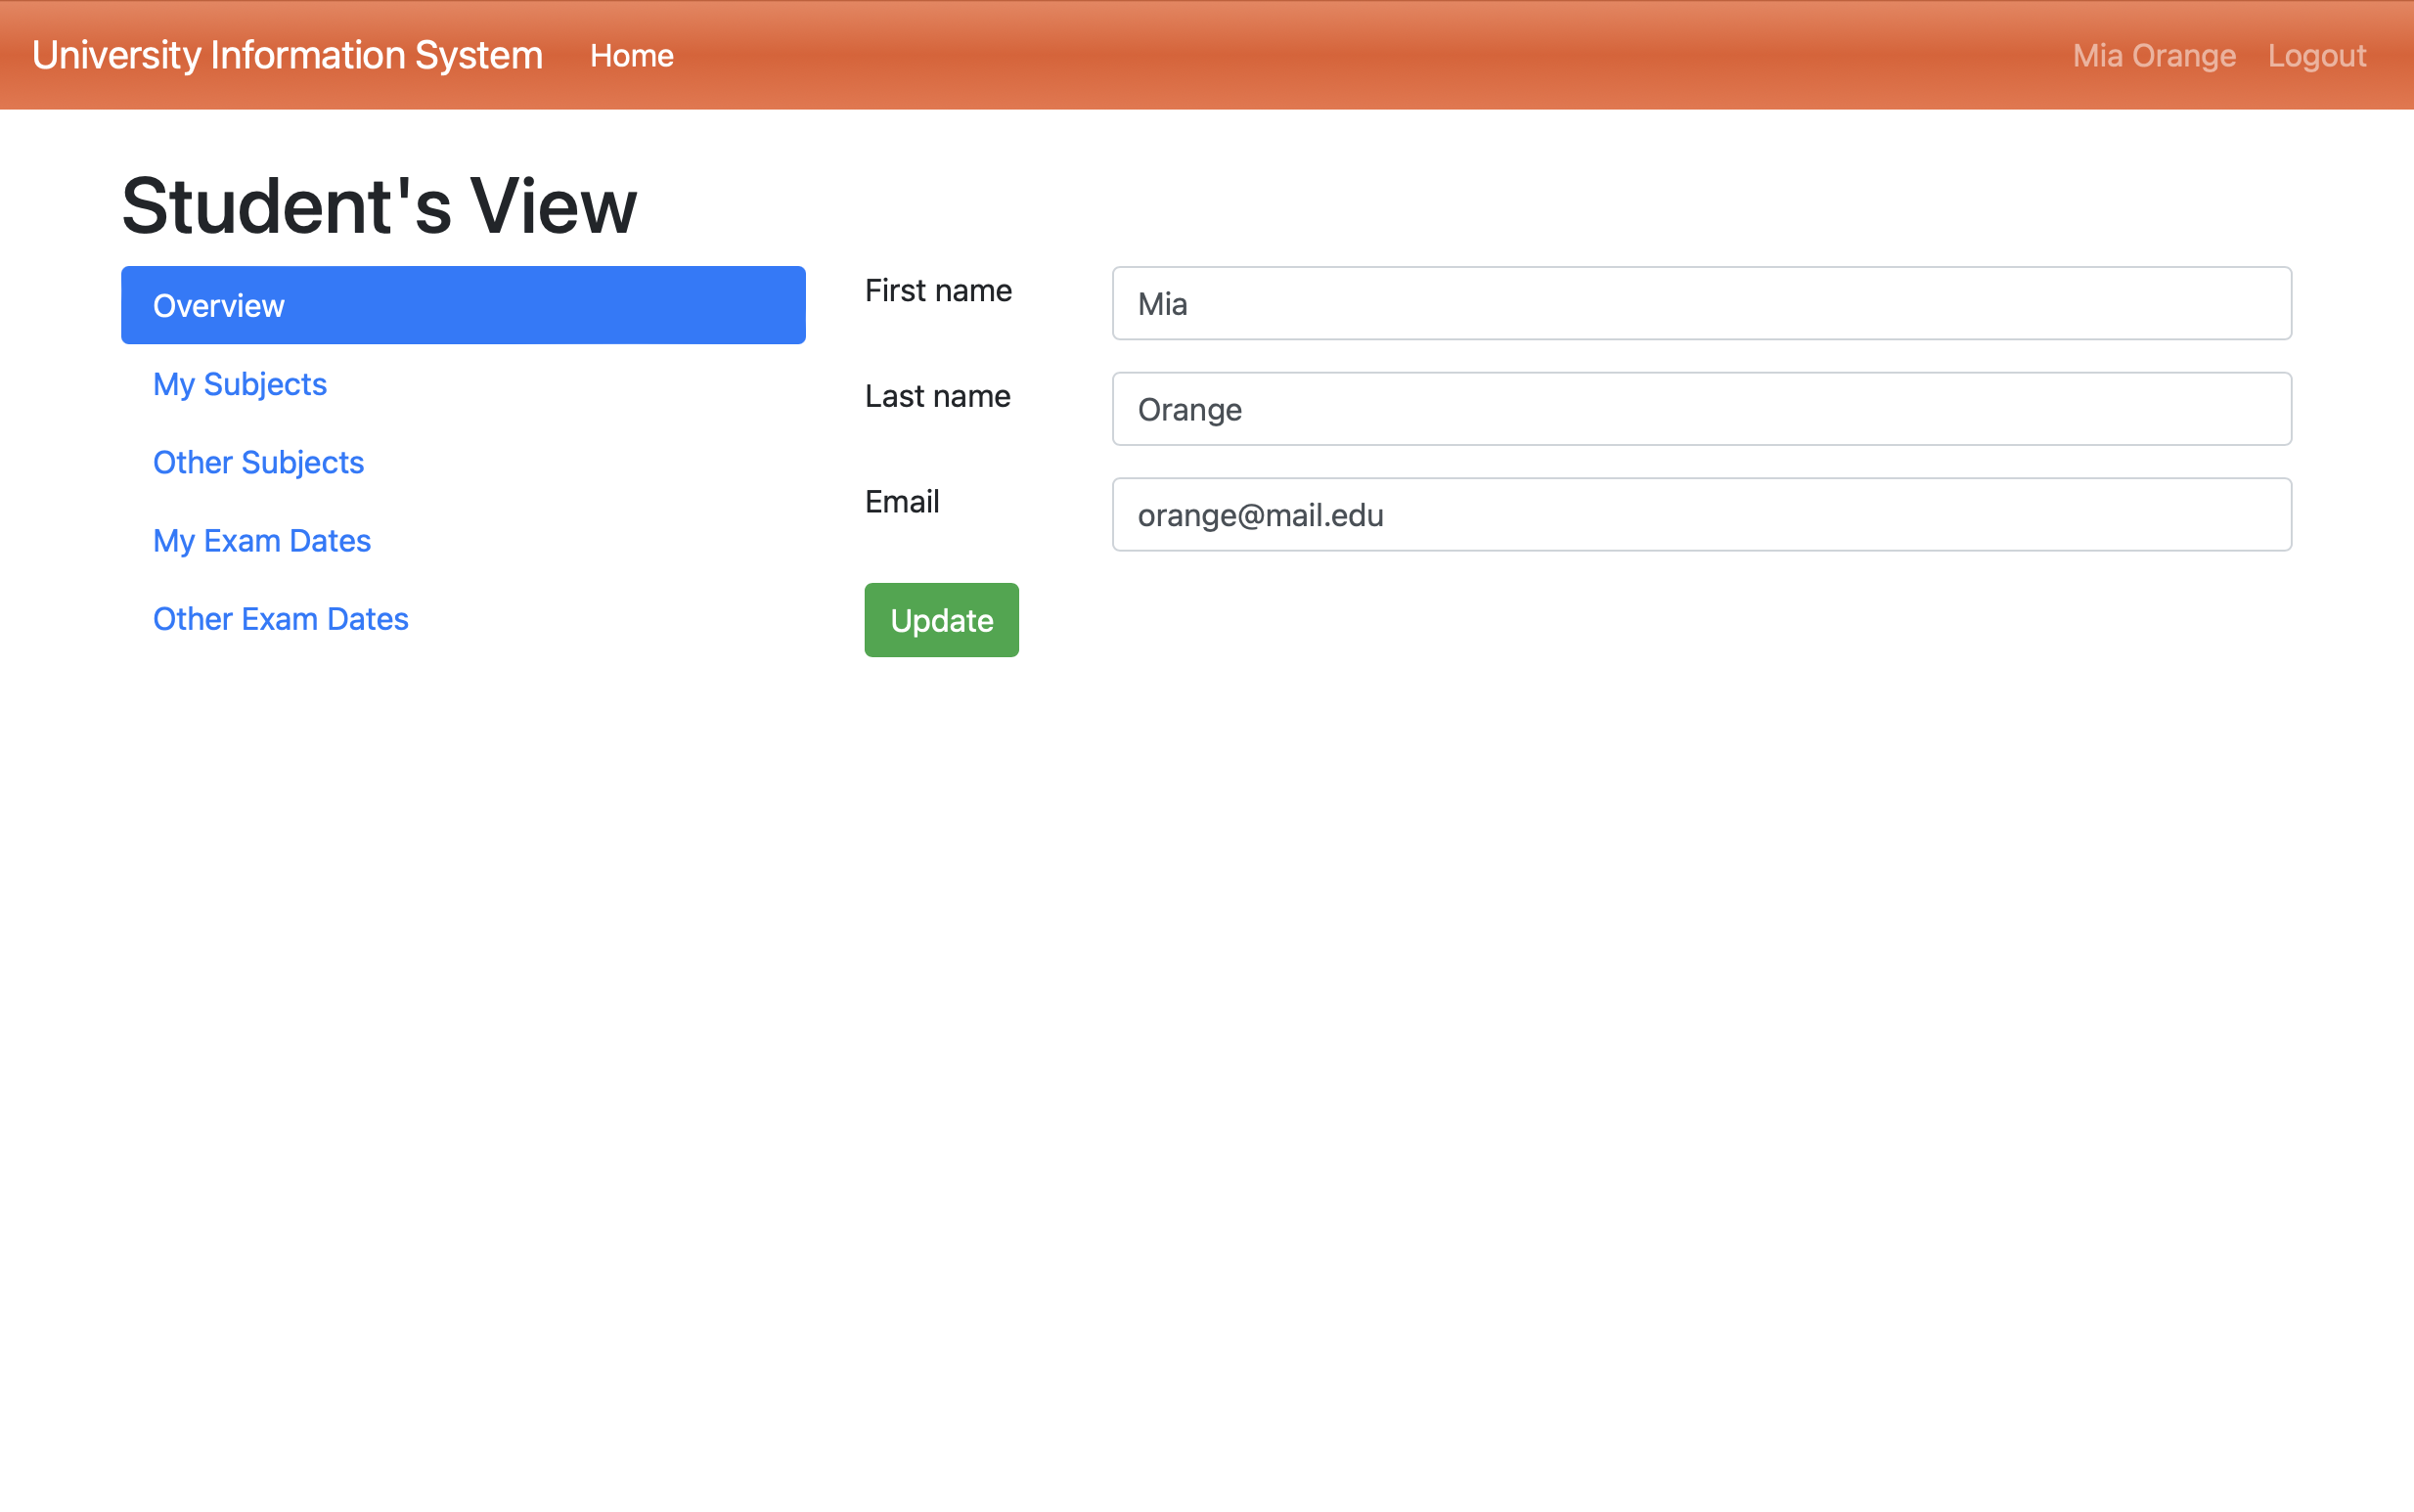
\includegraphics[width=0.8\textwidth]{pic/tbuis.png}
        \centering
        \caption{Prostředí systému TbUIS z pohledu studenta.}
        \label{fig:tbuis}
    \end{figure}

\chapter{Návrh}

        \section{Výběr cíle a metody testů} \label{sec:goals}
        V rámci této práce se chceme zaměřit nejen na možnost generování softwarových testů za pomocí \Gls{llm} a jeho proveditelnosti, ale také na jejich schopnost odhalit možné problémy, které se mohou objevit a jsou proti specifikaci daného testu nebo mimo ni. Toho chceme docílit nejen vygenerováním testů a srovnáním jejich vlastností a výsledků s testy napsanými člověkem, ale také narozdíl od v současnosti dostupných prací na podobné téma máme v plánu sputit testy nejen na validním kódu testovaného softwaru (aplikace), ale také zkusit do zdrojového kódu injektovat chyby a ověřit, zda výstupy testů z \Gls{llm} jsou schopné tyto chyby detekovat a také analyzovat tyto výstupy a jejich případné nedostatky. Předpokladem zde je, že testy predikované modelem budou více verbózní a pravděpodobně komplexnější než lidsky napsané testy, avšak funkcionalita (resp. její ověření na testované aplikaci) by měla v nejlepším případě být jak mezi \textit{strojovými} tak \textit{lidsky napsanými} testy shodná. Jeden rozdíl, který v základu volíme je, že naše \textit{strojové} testy jsou parametrizovány v rámci promptu a nepředpokladá se od nich (ani nevyžaduje) možnost načítat paramery za chodu jako mohou mít \textit{lidsky napsané} testy. Za parametry se mohou považovat například vstupní hodnoty, které testy využívají, případně hodnoty assertů (například v kombinaci se sadou vstupních parametrů) a podobně.

        Jako druh testů jsme zde zvolili GUI testování webových stránek (resp. aplikace) s využitím nástroje \textit{RobotFramework} a knihovny \textit{SeleniumLibrary}. Nejedná se tedy o klasický případ \textit{jednotkových} testů, ale stále má podobný rozsah, i když se dá říci, že vygenerované testy již mají přesah do integrační fáze. Zvolený druh testování byl vybrán i z důvodu, protože díky němu může tato práce navazovat na předchozí univerzitní projekt \textit{TbUIS}, popsaný v sekci \ref{sec:test_program}, který přesně vyhovuje našemu požadavku pro \emph{injekci chyb} a vznikl přesně pro tyto případy \gls{benchmark}ingu softwarových testů. Robot Framework je rozhraní postavené nad Pythonem, využívající vlastní jazyk pro zápis testů, který využívá příkazy v podobě tzv. \textit{klíčových slov}, které poskytují buďto poskytnuté knihovky nebo je lze definovat i v rámci testového souboru. Umožňuje také importovat a spuštět klasické Python moduly či podle nich definovat objekty. Jednotlivé testovací \textit{scénáře} se poté definují jako \uv{Test Cases}. Jak pro \textit{klíčová slova} tak \textit{scénáře} či \textit{nastavení} je potřeba tuto sekci kódu oddělit, jak lze vidět v příkladu \ref{lst:robot_example}. Lze také importovat např. klíčová slova či testovací data z externích skriptů jako je ukázáno na řádce 3. Podobně jako v běžných programovacích jazycích lze u klíčových slov definovat \emph{argumenty}. Stejně tak jsou podporovány proměnné, které mohou být deklarovány např. jako konstanty (viz řádka 5) nebo použity přímo v kódu pro uložení výstupu klíčového slova (řádka 16 ukázky). Jednotlivé výrazy jsou od sebe odděleny \textit{tabulátorem}, případně jiným podporovaným znakem.
        
        \begin{code}{robot}{Příklad struktury RobotFramework testu. \label{lst:robot_example}}
*** Settings ***
Library    SeleniumLibrary
Resource   keywords.resource

*** Variables ***
${URL}    https://example.com
${BROWSER}    Chrome

*** Test Cases ***
Open Website and Check for Text
    [Setup]    Open Browser    ${URL}    ${BROWSER}
    Page Should Contain    Welcome to Example Domain
    [Teardown]    Close Browser

Check User Name
    ${name}=    Get User Name
    Should Be Equal    ${name}    ${exp_full_name}

*** Keywords ***
Open Browser
    [Arguments]    ${url}    ${browser}
    Open Browser    ${url}    ${browser}
    Maximize Browser Window\end{code}

        Výsledným cílem práce je tedy předpokládán nástroj pro vygenerování jednotkových testů využívající Robot Framework na bázi uživatelské specifikace. Tento nástroj by také měl být schopen otestovat vygenerované testy dle daných specifikací na požadovaných variantách testované aplikace, mezi kterými budou klony u kterých je i není očekávané selhání testu. Tyto výsledky budou na konci vyhodnoceny pro různé \Gls{llm} modely a bude určeno, které z modelů dokáží generovat testy s co nejvyšší úspěšností detekce chyb a také je možno takovýto přístup využít v navazujících pracích, které by popisovanou generaci testů využívali.

        \section{Navrhované řešení} \label{sec:proposal}

        Řešení by v návrhu mělo fungovat jako softwarová \emph{pipeline}, tedy řetězec úkonů, které na sebe v rámci automatizovaného pracovního postupu musí navazovat, aby docílili určitého výsledku, za který v tomto případě považujeme \textit{otestovaný software}, zatímco jednotlivé vygenerované testy a jejich varinaty se berou jako mezivýsledky. Celý návrh pipeline je zobrazen na obr. \ref{fig:pipeline}. Kompletní proces začíná tím, že uživatel vytvoří s pomocí nástroje záznam prostupu webovou stránkou, tedy dokument, který obsahuje, na které prvky kliká či s nimi jinak interaguje a v jakém pořadí či časovém intervalu. Zároveň je od uživatele očekáváno, že označí nebo si poznamená prvky (např. dle jejich identifikátoru) od kterých je očekávána nějaká hodnota nebo chování (assert). Poté uživatel za pomocí orchestračního programu vytvoří nový test, nebo spíše šablonu podle které ho bude model generovat. Vyvořená šablona bude uživatelem doplněna o záznam (přesněji \textit{odkaz na něj}) a také doplněna o podmínky pro testovaní, které byli během záznamu poznamenány nebo vycházejí ze specifikace, dle které je testovací sénář (nebo přesněji test) tvořen. Doplněná šablona poté tvoří \emph{prompt} pro model.

        Po přesném specifikování podoby testu lze přistoupit k jeho \emph{generování}, při kterém se \Gls{llm} model dotazuje vytvořeným \emph{promptem} a je očekáváno vygenerování \(x\) tokenů, které lze považovat za vytvořeý test, případně při detekci nevhodných tokenů lze přistoupit k případné validaci či filtrování. Samozřejmostí také je, že uživateli je do vytvořeného testu umožněno nahlédnout a při viditelné chybě generovaného kódu i připustit manuální zásah a úpravu (nebude využito v této práci, jde jen o diskutovanou možnost). Samotné vytvoření testu a jeho generování je možné opakovat pro každý potřebný scénář či testový případ, který uživatel potřebuje vytvořit, než nastane další krok.

        Tímto dalším krokem je již samotné \emph{spuštění testů}, kterému však musí předcházet \emph{nasazení testované aplikace} a to v různých variantách. V rámci tohoto procesu bude vždy nasazena jedna varianta aplikace, poté spuštěny veškeré požadované testy, uloženy výsledky a program přejde k další variantě testovaného programu. Zmíněné kroky je také možno parametrizovat dle požadavků uživatele. Na konci pipeline by měl uživatel být schopen vyhodnotit výsledky a to jak programaticky tak manuálně.

        \begin{figure}
            \begin{tikzpicture}[node distance=2cm, auto]
                    \node (start) [block, fill=red!30] {Nahrávka a značkování};
                    \node (in1) [block, below of=start, fill=blue!30] {Vytvoření testu};
                    \node (pro1) [block, below of=in1, fill=gray!50] {Úprava promptu};
                    \node (pro2) [block, below of=pro1, fill=gray!50] {Generování};
                    \node (out1) [block, below of=pro2, fill=gray!50] {Zobrazení};
                    \node (pro3) [block, below of=out1, fill=gray!50] {Manualní úprava};
                    \node (dec1) [block, below of=pro3, fil=orange] {Validace testu};
                    \node (pro4) [block, below of=dec1, fill=blue!30] {Nasazení serverů a spuštění testů};
                    \node (stop) [block, below of=pro4, fill=green!50] {Vyhodnocení výsledků};

                    \draw [arrow] (start) -- (in1);
                    \draw [arrow] (in1) -- (pro1);
                    \draw [arrow] (pro1) -- (pro2);
                    \draw [arrow] (pro2) -- (out1);
                    \draw [arrow] (out1) -- (pro3);
                    \draw [arrow] (pro3) -- (dec1);
                    \draw [arrow] (dec1) -- (pro4);
                    \draw [arrow] (pro4) -- (stop);
            \end{tikzpicture}
            \centering
            \caption{Návrh pipeline projektu.}
            \label{fig:pipeline}
        \end{figure}

\chapter{Generování testů} \label{sec:test_generation}

    \section{Prerekvizity pro generování a spuštění testů}

    Pro spuštění projektových programů jsou vyžadovány následující softwarové a hardwarvé prerekvizity:
    \begin{itemize}
        \item\textbf{Spuštění testů}
           \begin{itemize}
                \item \textbf{Operační systém} - Program je navržený pro \uv{UNIX-like} operační systémy (Linux, MacOS), které jsou pro jeho spuštění vyžadovány. V případě operačního systému Windows je doporučeno využít technologii \textbf{WSL2}.
                \item \textbf{Docker Desktop} (včetně Docker Compose).
                \item \textbf{Python 3.11} nebo vyšší (z důvodu kompatibility některých frameworků).
                \item \textbf{Robot Framework} společně s knihovnou \textit{SeleniumLibrary} jako Python moduly.
                \item V případě, že se společně s Robot Framework nenainstaluje, je také potřeba přidat Chrome nebo Chromium driver.
                \item Přítomný display server (nelze spouštět na čistě CLI systémech).
           \end{itemize} 
       \item\textbf{Lokální spouštění LLM} (generování testů)
           \begin{itemize}
                \item \textbf{Operační systém} - Libovolný.
                \item \textbf{Hardware} - CPU s podporou AVX2 instrukční sady, minimum 16GB RAM, v případě běhu na VGA doporučeno alespoň 6GB VRAM.
                \item Nainstalovaný software \textbf{LM Studio}.
           \end{itemize}
    \end{itemize}

    \section{Výběr scénářů} \label{sec:scenarios}

    Pro vygenerování testů za pomocí LLM bylo nejdříve nutné vybrat ze sady \textit{use caseů}\footnote{Seznam dostupný na adrese: \url{https://projects.kiv.zcu.cz/tbuis/web/page/uis#use-cases}} scénáře vhodné pro demonstraci nejen správné funkčnosti, ale také s možností ověření nesprávného chování na poruchových klonech (diskutováno v sekci \ref{sec:test_program}). Požadavek tedy byl, aby většina z vybraných scénářů vycházející z \textit{use casu} měl alespoň jeden poruchový klon, případně více. Vybráno bylo \(10\) scénářů, testovaných celkově na \(14\) variantách programu. Seznam vytvořených specifikací pro automatické generování testů se nachází v tabulkách \ref{tab:specs_1} a \ref{tab:specs_2}. Scénáře budou dále také referovány jako \textit{specifikace}. Každá specifikace má \textit{číslo}, které odpovídá číslu \textit{use casu}, ze kterého vychází (např. specifikace \(04\) vychází z use casu \textit{UC.04}). Zde je nutné poznamenat, že ne všechny specifikace vychází pevně z jejich use casů, ale byli upravené tak, aby šli provést v jednom chodu bez nutných závislostí (\textit{jako například namísto podmínky přihlášeného uživatele se uživatel vždy musí na začátku či během testu přihlásit do systému}). Popis specifikací v tabulce je pouze orientační a pro bližší upřesnění jednotlivých kroků, které se mají provést referujte web projektu. V tomto seznamu se také u každé specifikace nachází výčet klonů, na kterých lze očekávat poruchu. Celkový seznam klonů, a kterých se budou všechny vytvořené testy spouštět lze nalézt v tabulce \ref{tab:clones}. Podobně jako v případě specifikací, čísla klonů odpovídají číslům, jak jsou uvedena na oficiálním webu\footnote{Seznam poruchových klonů společně s možností stažení: \url{https://projects.kiv.zcu.cz/tbuis/web/page/download}} projektu společně s vysvětlením jednolivých chyb varianty. Pro přehlednost jsme bezchybnou variantu označili číslem \(00\).

    \begin{table}
        \begin{tabular}{|c|p{7cm}|c|}
            \hline
            \textbf{Specifikace} & \textbf{Popis} & \textbf{Porucha na klonech} \\
            \hline
            \(1\) & \textit{Přihlášení do aplikace} \newline Student i učitel se přihlásí do aplikace přihlašovacími údaji, dostupnými v databázi systému. Dále se zkontroluje, zda systém pro účet s neexistujícím uživatelským jménem nebo neplatným heslem vypíše chybovou hlášku. &  \(02\) \\
            \hline
            \(4\) & \textit{Odepsání předmětu} \newline Student se přihlásí, odepíše předmět v patřičné sekci systému. Předmět by následně měl zmizet v ostatních sekcích a to jak v pohledu studenta tak učitele. & \(04, 19, 25, 26, 28\) \\
            \hline
            \(6\) & \textit{Zapsání předmětu} \newline Student se přihlásí, zapíše předmět v patřičné sekci, který se následně zobarazí i v ostatních částech systému. Z učitelského pohledu by se student měl zobrazit na seznamu studentů daného předmětu. & \(25, 26, 28\) \\
            \hline
            \(8\) & \textit{Registrace na zkoušku} \newline Student se přihlásí do systémů a zapíše se na jeden z možných zkouškových termínů. Tento termín by se měl přesunout mezi již zapsané termíny. V učitelském pohledu bude student na seznamu zapsaných na konkrétní zkoušku a také by mělo být možno studenta ohodnotit. & \(22, 25, 26, 28\) \\
            \hline
            \(9\) & \textit{Zobrazení spolužáků u zkoušky} \newline Student se přihlásí a u zkoušky si může rozkliknout seznam všech účastníků. & \(\) \\
            \hline
            \(10\) & \textit{Zrušení předmětu} \newline Učitel po přihlášení klikne na tlačítko \textit{Remove} u předmětu, od jehož výuky se chce odhlásit. Ten se přestane zobrazovat ve všech ostatních sekcích systému z jeho pohledu, až na jeho znovuzapsání. Student by u předmětu neměl najít jméno daného učitele, který se odhlásil. & \(26, 28\) \\
            \hline
            \(11\) & \textit{Zobrazení studentů u předmětu} \newline Učitel se přihlásí do systému a u předmětu je schopen si zobrazit seznam zapsaných studentů. & \(26, 28\) \\
            \hline
        \end{tabular}
        \centering
        \label{tab:specs_1}
        \caption{Specifikace pro generované testy - část 1}
    \end{table}

    \begin{table}
        \begin{tabular}{|c|p{7cm}|c|}
            \hline
            \textbf{Specifikace} & \textbf{Popis} & \textbf{Porucha na klonech} \\
            \hline
            \(12\) & \textit{Zrušení zkoušky} \newline Učitel se přihlásí a v sekci jeho přidělených zkoušek odstraní konkrétní termín. Tento termín by nyní neměl být vidět jak v učitelském tak studentském pohledu do systému. & \(20, 21, 23, 26, 28\) \\
            \hline
            \(17\) & \textit{Přihlášení se k výuce předmětu} \newline Učitel se přihlásí do systému a v seznamu předmětů se přihlásí k výuce daného předmětu. Ten by se poté měl zobrazit ve zbytku systému v rámci patřičných sekcí. Zároveň studenti by nyní měli u předmětu vidět jméno tohoto vyučujícího. & \(18, 24, 25, 26, 27, 28\) \\
            \hline
            \(18\) & \textit{Zobrazení seznamu učitelů a předmětů, které vyučují} \newline Přihlášený učitel je schopen si zobrazit seznam všeech učitelů. & \(27, 28\) \\
            \hline
        \end{tabular}
        \centering
        \label{tab:specs_2}
        \caption{Specifikace pro generované testy - část 2}
    \end{table}

    \begin{table}
        \begin{tabular}{|c|c|}
            \hline
            \textbf{Číslo klonu} & \textbf{Porucha} \\
            \hline
            \(00\) & Bez defektu \\
            \hline
            \(02\) & Překlep v nadpisu \\
            \hline
            \(04\) & Návrat na špatnou stránkau\\
            \hline
            \(18\) & Chybějící sloupec v tabulce \\
            \hline
            \(19\) & Náhodně chybějící tlačítko \\
            \hline
            \(20\) & Nefunkční tlačítko \\
            \hline
            \(21\) & Změna se nepropíše do UI \\
            \hline
            \(22\) & Nefunkční tlačítko \\
            \hline
            \(23\) & Smazání se nepropíše do DB \\
            \hline
            \(24\) & Přidání se nepropíše do DB \\
            \hline
            \(25\) & Tabulka studentů prázdná \\
            \hline
            \(26\) & Tabulka učitelů prázdná \\
            \hline
            \(27\) & Nesprávný výběr z DB \\
            \hline
            \(28\) & Mix chyb (včetně interní chyby systému) \\
            \hline
        \end{tabular}
        \centering
        \label{tab:clones}
        \caption{Seznam poruchových klonů využitých pro testování.}
    \end{table}

    \section{Nahrávání scénářů}

    Dle \emph{specifikace} z předchozího bodu, vytvoří uživatel LLM generačního nástroje nahrávku jednotlivých kroků, které má test provést. V případě, že specifikace udává více uživatelských pohledů (\textit{student / učitel}), nahraje uživatel tyto pohledy jednotlivě. Současný projekt pracuje s nahrávacím nástrojem v rámci vývojářských nástrojů webového prohlížeče \textit{Google Chrome} (pro vývoj byla využita verze \(124\)). Tento nástroj je stále experimentální funkce, takže nelze vyloučit možnost, že v následujícíh verzích již nemusí být dostupný. Díky této funkci lze nahrávat uživatelské vstupy a interakce s jednotlivými prvky v rámci webových stránek. Mimo jiné také umožňuje přidávat \textit{asserty}, avšak tyto možnosti jsou nedostatečné a tedy v rámci této práce se omezíme pouze na údaje o interakci s prvky. Nahrávání zobrazeno na obr. \ref{fig:chrome_recording}. Nástroj je schopen vyexportovat výstup nahrávání v řadě formátů. Zde jsme zvolili JSON formát, který popisuje jednotlivé akce dle objektů. Nahrané scénáře uživatel vhodně pojmenuje a uloží do složky \verb|input| programu, který je součástí tohoto projektu. Vytvořený program pro generování testů za pomocí LLM se stará o veškerou orchestraci generování i spouštění testů a také vytovření \emph{šablon} pro testy, ze kterých se generují. Součástí těchto \emph{šablon} je právě i uživatelova nahrávka. Ukázkovou strukturu \verb|input| složky lze vidět ve výpisu \ref{con:input}, kde se nachází \emph{šablona} pro \textit{specifikace} \(1\) a \(4\). Význam \emph{šablon} je diskutován v následující sekci.

    \begin{figure}
        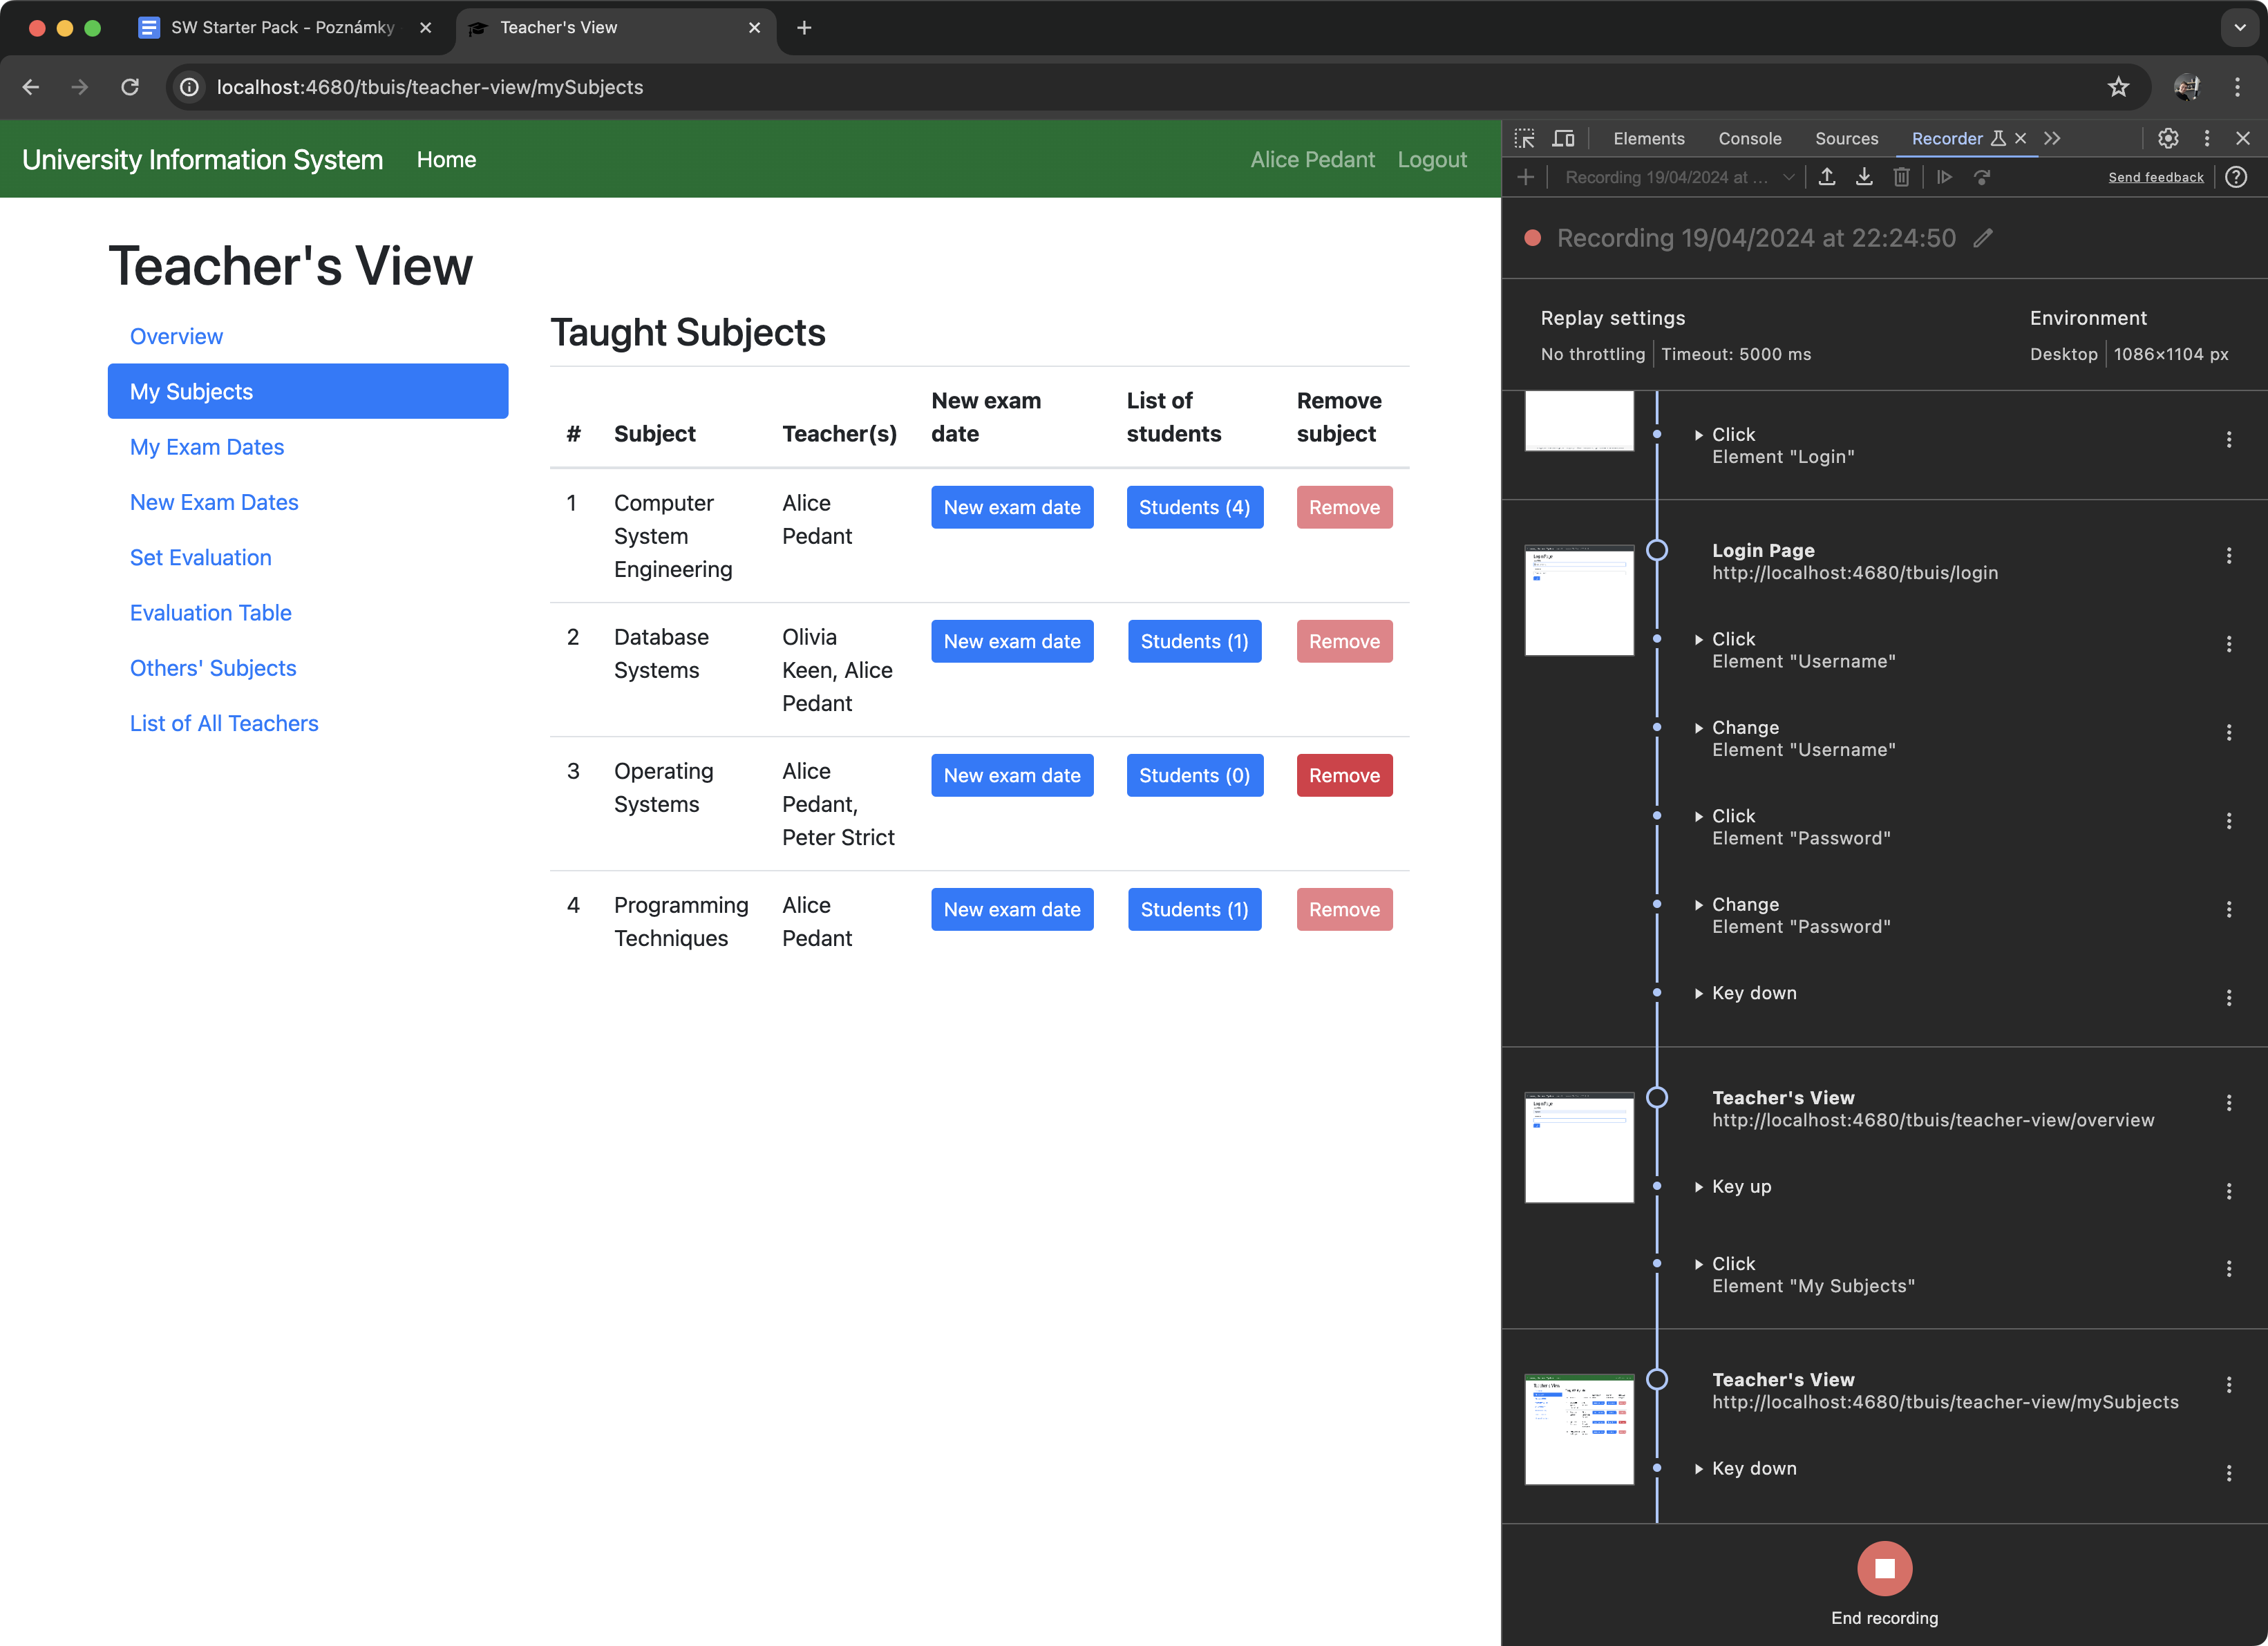
\includegraphics[width=0.8\textwidth]{pic/recording.png}
        \centering
        \caption{Nahrávání scénáře za pomocí nástroje v Google Chrome}
        \label{fig:chrome_recording}
    \end{figure}

    \newpage
    \setuxprompt{milan}{dp/program/input}
    \begin{console}{Ukázková struktura input složky \label{con:input}} 
`\uxprompt`ls -l
milan    448 Apr 21 20:52 ..
milan   3815 Mar 27 20:24 rec-spec-1-student.json
milan   3820 Mar 27 20:28 rec-spec-1-teacher.json
milan   6043 Mar 30 19:42 recording-spec-4-student.json
milan  10635 Mar 31 09:18 recording-spec-4-teacher.json
milan   1370 Apr 21 20:52 spec-1.txt
milan   1328 Mar 31 09:28 spec-4.txt
    \end{console}

    \section{Výběr požadavků}

        \subsection{Vytvoření nového testu} \label{sec:test_creation}

            Primárním programem celé práce je soubor \verb|test.py|, který se nalézá v kořenové složce programu (\verb|/program|) a má konrétně 3 pracovní režimy:
            \begin{enumerate}
                \item Vyvtvoření šablony pro test
                \item Vygenerování testu dle šablony
                \item Spuštění sady testů
            \end{enumerate}
            Právě první režim je v současném kroce důležitý. Jednotlivé režimy programu jsou spuštěny za pomocí argumentů (argumenty jednotlivých režimů ukázané ve výpisu \ref{con:modes}). V případě \textit{vytvoření} nového testu se za argument přidává název šalony testu. Tento název musí být unikání a využívá se později ve zbytku programu jakožto identifikátor daného testu. Po potvrzení příkazu se ve vstupní složce vytvoří nová šablona pro test se zvoleným názvem a příponou \verb|.txt|. Tuto šablonu může uživatel může dále upravit. Celý příkaz je ukázaný ve výpisu \ref{con:new}. Vytvořenou šablonu uživatel zobrazí a upraví v \textit{textovém editoru}.

            \vfill

            \begin{console}{Hlavní režimy programu \label{con:modes}}
`\uxprompt`python3 test.py -n   #Nový test
`\uxprompt`python3 test.py -i   #Generování
`\uxprompt`python3 test.py -r   #Spuštění testů
            \end{console}

            \begin{console}{Vytvoření nového testu (šablony) \label{con:new}}
`\uxprompt`python3 test.py -n specficication-1
            \end{console}

                \begin{code}{text}{Vzor pro vyplnění šablony testu \label{lst:template}}
Write Robot Framework scanario. Open page like in this JSON recording and then when you execute all the steps in the recording, do this:

- //TODO


                \end{code}

                \begin{code}{text}{Vyplněná šablona testu pro specifikaci 18 \label{lst:spec18}}
Write Robot Framework scanario. Open page like in this JSON recording and then when you execute all the steps in the recording, do this:

- Check if there are these names present on the page: Julia Easyrider, Olivia Keen, John Lazy, Alice Pedant, Thomas Scatterbrained, Peter Strict
- Check if element with path //*[@id="tea.listOfAllTeachers.table.teacherRow-0"]/td[3] has text matching "Numerical Methods"
- Check if element with path //*[@id="tea.listOfAllTeachers.table.teacherRow-1"]/td[3] has text matching "Database Systems, Fundamentals of Computer Networks, Introduction to Algorithms, Mobile Applications, Web Programming"
- Check if element with path //*[@id="tea.listOfAllTeachers.table.teacherRow-2"]/td[3] should not contain text
- Check if element with path //*[@id="tea.listOfAllTeachers.table.teacherRow-3"]/td[3] has text matching "Computer System Engineering, Database Systems, Operating Systems, Programming Techniques"
- Check if element with path //*[@id="tea.listOfAllTeachers.table.teacherRow-4"]/td[3] has text matching "Computation Structures"
- Check if element with path //*[@id="tea.listOfAllTeachers.table.teacherRow-5"]/td[3] has text matching "Operating Systems, Programming in Java, Software Engineering, Software Quality Assurance"


                \end{code}

                \subsection{Vyplnění požadavků}

            Do šablony je vložen základní prompt společně s požadavky, které uživatel může vyplnit (viz ukázka \ref{lst:template}). Pod požadavky je defaultně vložena nahrávka \verb|recording.json|. Tuto hodnotu nahradí uživatel za název souboru vložené nahrávky. Formát šablony jakožto vstupu pro prompt testu byl zvolen pro jednodušší parametrizaci. Šablona využívá jazyk \emph{Jinja2}. V rámci vytvořených šablon v této práci byly tyto parametrizační vlastnosti využity například pro vytvoření pohledu \textit{studenta} a \textit{učitele}. Místo, které je v šabloně označeno jako \verb|\\TODO| slouží pro napsání požadavků testu. Od uživatele se čeká, že tyto požadavky vypíše v odrážkách, čemuž odpovídá i formát \emph{promptu}. Ukázka vyplněných požadavků pro konkrétní test je součástí výpisu \ref{lst:spec18}, který ukazuje vypsané vlastnosti pro specifikaci 18, jak bylo popsáno v sekci \ref{sec:scenarios}.


    \section{Dotazování LLM}

        \subsection{Modely a jejich spuštění}
            %Co za modely bylo zvoleno, jejich druhy, atd.
            
            Jak již bylo řečeno v kapitole \ref{sec:research}, velké jazykové modely existují jak v prorietární formě, které jsou dostupné pouze přes API poskytovatele nebo webové rozhraní, ale také se dají najít modely dostupné v \textit{public} či \textit{open source} formě dále referovány jako \emph{otevřené} modely). V rámci tohoto projektu byly využity obě varianty, tedy \emph{proprietární} modely srkze API poskytovatele a otevřené lokálně nebo také srze API u některého z poskytovatelů a to z důvodu vysokých hardwarových nároků některých modelů.Konkrétní seznam použitých modelů v práci včetně typu přístupu k nim lze nalézt v tabulce \ref{tab:used_models}. Pro dotazování vzdálených modelů využívá většina koncových bodů API od OpenAI, tedy jsou kompatibilní s jejich knihovnou pro různé jazyky. Některé společnosti však pro své modely využívají vlastní definici API, mezi ně se řadí například \textit{Anthropic} nebo \textit{Google}. V projektu tedy využíváme pro veškteré kompatibilní modely (resp. jejich běhová prostředí) knihovnu pro OpenAI API, se kterým jsou kompatibilní, a pro zbytek jejich vlastní knihovny.

            \begin{table}
                \catcode`\-=12
                \begin{tabular}{|c|c|p{5cm}|c|}
                    \hline
                    \textbf{Tvůrce} & \textbf{Model} & \textbf{Použitá verze} & \textbf{Runtime} \\
                    \hline
                    \multirow{3}{*}{OpenAI} & GPT-4 & gpt-4-32k & \multirow{3}{*}{API} \\
                    \cline{2-3} 
                    & GPT-4 Turbo & gpt-4-turbo-2024-04-09 &  \\
                    \cline{2-3} 
                    & GPT-3 Turbo & gpt-3-turbo-0125 &  \\
                    \hline
                    \multirow{2}{*}{Mistral} & Mixtral 7B & TheBloke/Mistral-7B-Instruct-v0.2 & Lokální \\
                    \cline{2-4} 
                     & Mistral Large & mistral-large-2402 & API \textit{La Plateforme} \\
                    \hline
                    Anthropic & Claude 3 Opus & claude-3-opus-20240229 & API \\
                    \hline
                    \multirow{3}{*}{Meta} & Codellama & TheBloke/Phind-CodeLlama-34B-v2 & \multirow{3}{*}{Lokální} \\
                    \cline{2-3}
                     & Llama 3 70B & MaziyarPanahi/Meta-Llama-3-70B-Instruct & \\
                    \cline{2-3}
                     & WizzardCoder & TheBloke/WizardCoder-Python-34B-V1.0 & \\
                    \hline
                    Google & Gemini 1.5 Pro & gemini-1.5-pro-preview-0409 & API \textit{Google Cloud} \\
                    \hline
                \end{tabular}
                \centering
                \caption{Použité LLM modely}
                \label{tab:used_models}
            \end{table}

            \subsubsection{Prostředí pro lokální modely} \label{sec:local_env}

            Pro \emph{lokální} modely a jejich spuštění byl využit software \textit{LM Studio}, který je postaven nad \textit{C++} knihovnou \verb|llama.cpp|. Ta umožňuje jednoduché spuštění \Gls{llm} modelů ve formátu \acrfull{gguf}. Jedná se o \textit{binární} formát souborů určený pro rychlé načítání a ukládání modelů využíváných pro účely interferenčních úloh. Jeho návrh umožňuje snadnou úpravu při zachování zpětné kompatibility. \cite{ggerganov_gguf} \cite{huggingface_gguf} Modely mohou být vyvíjené za pomoci různých frameworků (např. \textit{PyTorch}) a poté převedeny do \acrshort{gguf} formátu pro použití v rámci \acrshort{ggml} knihovny, která umožňuje efektivní spuštění modelů na CPU a GPU. Knihovna také umožňuje \emph{kvantizaci}, tedy techniku využívanou ke snížení paměťových nároků \acrshort{ml} úloh. Zahrnuje reprezentaci vah a aktivací za pomoci datakových typů s nižší přesností (např. \textit{int8}) oproti obvyklým 32 bitovým číslům (např. \textit{float32}), ve kterých bývají reprezentována originální data modelu. Jejím cílem je snížit počet bitů, což vede k nižší velikosti modelu a to k nižším HW nárokům a s tím spojených vlastností (\textit{snížená energetická spotřeba, nižší latence, ...}). Kvantizace má však i nežádoucí dopady a to \textit{ztrátu přesnosti} nebo případně \textit{výkonu} modelu. \cite{huggingface_quantization} \Acrshort{gguf} tedy tvoří jednotný formát, ve kterém se spousta otevřených \Gls{llm} modelů (případně jejich konverzí) distribuuje. Jednou z platforem pro jejich distribuci je například \href{https://huggingface.co}{HuggingFace}.

            \begin{figure}
                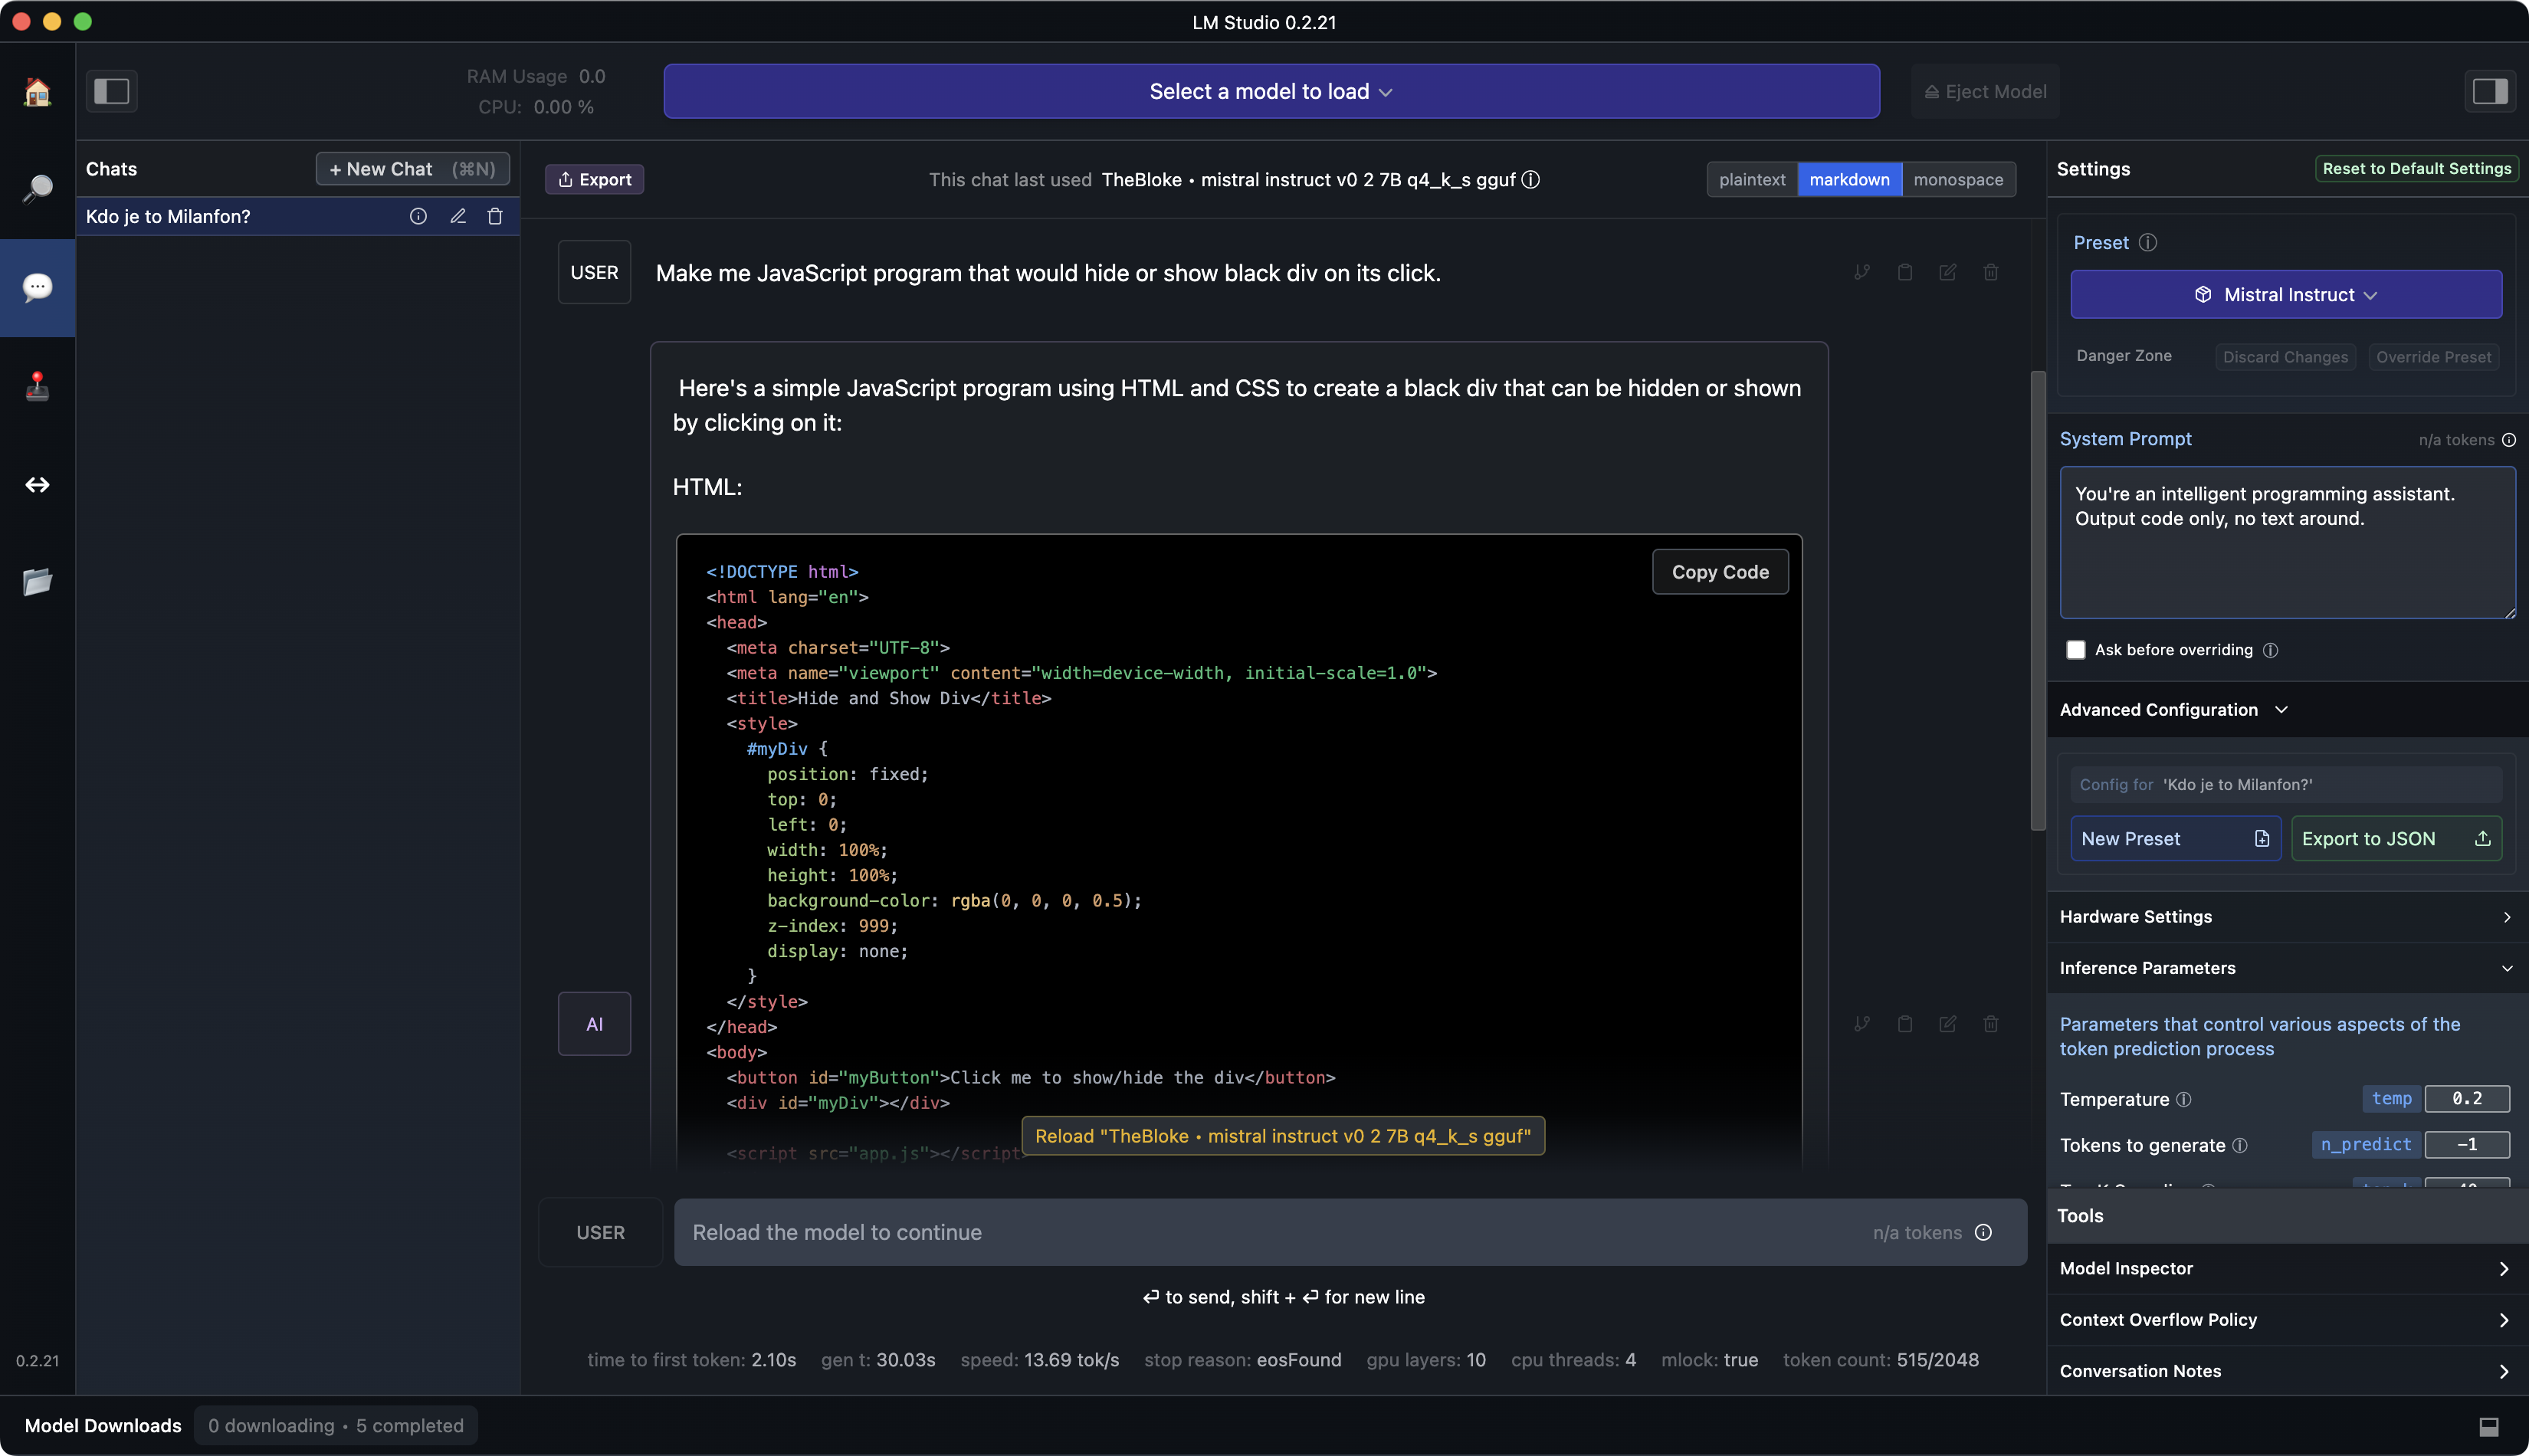
\includegraphics[width=\textwidth]{pic/lm_studio.png}
                \centering
                \caption{LM Studio}
                \label{fig:lm_studio}
            \end{figure}

            \textit{LM Studio} umožňuje spuštění právě modelů ve formátu \acrshort{gguf}, včetně jejich stažení z repozitářů a funkcemi s tím spojených (například \textit{vypsání seznamu kvantizací, spojení rozdělených modelů, atd.}). Jeho primární funkcí je spouštět lokální \Gls{llm} modely jako \textit{chat} nebo \textit{lokální server} nabízející API kompatibilní s definicí dle OpenAI. Pro každý druh modelů (jako \textit{Llama, Mistral, Command R, ...}) také obsahuje předdefinované nastavení, které si uživatel může upravit. Mezi tímto nastavením jsou hyperparametry jako \textit{\gls{temperature}, Min P, Top P, délka \gls{context}u, maximálního počtu vygenerovaných \gls{token}ů a dalších}. Mimo toho obsahuje i nastavení pro hardware jako \textit{počet vláken CPU, počet GPU vrstev, GPU framework} a podobně. \textit{Vrstvou} je zde myšlena vrstva neutronů, která provádí určit výpočty a zpracování vstupních dat. Vrstvy mohou být ku příkladu \textit{vstupní, skryté, výstupní}. Klíčovou vlastností nastavitelnou v rámci runtimu tohoto softwaru je možnost nastavit chování \gls{context}ového okna. Mezi možnosti se řadí: 
            \begin{enumerate}
                \item \textit{Klouzavé okno} - Model si pamatuje posledních \(x\) tokenů z konverzace, které využívá ke generování výstupu a predikci.
                \item \textit{Začátek a konec} - Model si pamatuje první prompt (případně i systémový) a zbylé tokeny na konci konverzace.
                \item \textit{Zastavení} - Při dosažení počtu tokenů v rámci konverzace rovnající se \(x\), je generování odpovědi zastaveno.
            \end{enumerate}
            Proměnnou \(x\) je zde myšlena celková délka kontextu, kterou \textit{model} nebo \textit{runtime} podporuje. V případě \textit{runtimu} v rámci \textit{LM Studio} (resp. \verb|llama.cpp|) může uživatel délku kontextu zvolit až do délky \(16 384\) \gls{token}ů. Pokud však tato délka bude větší, jak podporovaný kontext samotným modelem, délka kontextu, který model má v paměti, bude dán hodnotou z modelu. Například modely vycházející z architektury \textit{Llama-2} disponují kontextem \(4096\) \gls{token}ů, jak bylo diskutováno v sekci \ref{sec:research_models}. Pokud tedy runtime bude nastaven s větším kontextovým oknem, bude rozhodující právě tato hodnota modelu.
            
            Pro spuštěnou instanci modelu lze také nastavit \textit{systémový prompt}. Jedná se o první zprávu, která se modelu předává a měla by obsahovat pokyny pro model definující jeho chování, roli a další relevatní informace, které mohou zlepšit přesnost jeho výsledků nebo mu umožnit lépe pochopit kontext. Tento prompt je běžně vložen pouze na začátku konerzace a poté uložen do paměti modelu. Ukázku takového systémového promptu lze vidět ve výpisu \ref{lst:system_prompt_example}. Tento konkrétní příklad pochází právě ze softwaru \textit{LM Studio}.

            \begin{code}{text}{Příklad systémového promptu \label{lst:system_prompt_example}}
You're an intelligent programming assistant. Output code only, no text around.
            \end{code}

            \subsubsection{Testovací sestava a nastavení}

            \begin{table}
                \begin{tabular}{|c|c|}
                    \hline
                    \textbf{Typ} & \textbf{Komponenta} \\
                    \hline
                    CPU & AMD Ryzen 8700F \\
                    \hline
                    Základní deska & Asus B650-PLUS TUF \\
                    \hline
                    CPU Chlazení & BOX \\
                    \hline
                    RAM & Kingston FURY Renegade DDR5 64GB 6400 MHz (4x16GB) \\
                    \hline
                    VGA & Radeon RX 7900 XT 20GB Asus TUF \\
                    \hline
                    PSU & ADATA XPG CYBERCORE 1300W \\
                    \hline
                    Case & BeQuiet! Dark Base Pro 901 \\
                    \hline
                \end{tabular}
                \centering
                \caption{Seznam komponent testovací PC sestavy}
                \label{tab:pc_components}
            \end{table}

            Pro spouštění lokálních modelů byla využita PC sestava, jejíž komponenty jsou popsané v tabulce \ref{tab:pc_components}. Runtime programu \textit{LM Studio}, popsaného v minulé sekci, byl nastaven, aby využíval \(12\) z \(16\) dostupných CPU vláken. GPU akcelerace fungovala v režimu \textit{OpenCL}. Počet GPU vrstev se však liší model od modelu. Pro správnou funkčnost je potřeba udržet celý model v paměti RAM, tedy v případě naší sestavy jsme mohli pracovat s modely pouze cca do 60GB, s tím, že do VRAM grafické karty lze nahrát pouze vrstvy o celkové velikosti přibližně 20GB. Na GPU tedy byl akcelerován jen takový počet vrtev, který z jejich celkového počtu odpovídal této velikosti. Délka \textit{kontextového okna} byla nastavena na \(8 192\) \gls{token}ů, avšak pro některé modely je tato délka zkrácena samotným modelem (viz sekce \ref{sec:local_env}). Jednotlivé hyperparametry byly poté nastaveny jako:
            \begin{enumerate}
                \item \textbf{\gls{temperature}}: \(0.7\)
                \item \textbf{Top P}: \(1\)
                \item \textbf{Maximum vygenerovaných tokenů}: \(3000\)
                \item \textbf{režim kontextového okna}: klouzavé okno
            \end{enumerate}
            Zbytek \emph{hyperparametrů} zůstal na defaultních hodnotách daného modelu, který byl testovaný. Toto nastavení bylo využito jak pro \textit{lokální} modely tak pro \textit{API} dotazy na poskytovatele proprietáních či jiných vzdáleně spuštěných modelů. Použité hodnoty těchto parametrů vycházejí z prvotních testovacích experimentů, kdy se osvědčili jako vhodné pro generování jednotkových testů, protože by měli zaručovat \textit{nižší determiničnost} výsledku a jeho \textit{vyšší přesnost}.

        \subsection{Dotazy} \label{sec:llm_requests}
        Samotné vygenerování testů za pomoci dotazování \Gls{llm} je řešeno skrze \textit{generující} režim programu, jako je ukázáno ve výpisu \ref{con:modes}. Tento režim jako argument vyžaduje \textit{název šablony}, která funguje jako \textit{prompt} pro model a byla vytvořena v předchozím kroku (viz sekce \ref{sec:test_creation}). Tento režim poporuje i více nepovinných argumentů jako:
        \begin{itemize}
            \item \verb|count| - Počet variací testů, které se mají vygenerovat. Celé číslo. Defaultní hodnota \(1\).
            \item \verb|manual| - Zkopírovat prompt do schránky pro manuální vložení do rozhraní modelu. Vlajka. Vhodné pro debug.
            \item \verb|cmd| - Vypsat prompt do standardního výstupu. Vlajka.
            \item \verb|compress| - Vlajka vyjadřující použití promptové komprese.
        \end{itemize}

        Mimo argumentů je \textit{generování testů} také konfigurováno \textit{proměnnými prostředí}, které pokud nejsou definovány, program se snaží načíst soubor \verb|.env| (pokud je přítomný), který tyto proměnné obsahuje. Konfigurace generování za pomocí těchto proměnných byla zvolena, protože se většinou nepřidávají do \Acrshort{vcs} nebo je jejich přidání ošetřeno, protože obsahují citlivá data, která by měla zůstat pouze na stroji uživatele. Mezi základní proměnné prostřední patří:
        \begin{itemize}
            \item \verb|API_URL| - Adresa URL, na kterou program dělá API dotazy.
            \item \verb|API_KEY| - Klíč pro přístup ke vzdálenému API (pro lokální modely stačí zadat libovolnou hodnotu nebo nedefinovat).
            \item \verb|API_MODEL| - Název modelu, na kterém programu bude v rámci API požadovat vygenerování výstupu (hodnota dána dokumentací daného API).
            \item \verb|MAX_TOKENS| - Maximální počet tokenů, které má model vygenerovat. V závislosti na dokumentaci API je potřeba nastavit hodnotu v určiném rozsahu.
        \end{itemize}
        Mimo parametrů pro generování může \verb|.env| soubor obsahovat i další parametry (resp. proměnné) určené pro jiné operace programu. Ukázková podoba tohoto souboru je zobrazena ve výpisu \ref{lst:dot_env}. Soubor je umístěn v kořenové složce programu.

        Ukázkové volání programu v režimu generace testů lze vidět v ukázce \ref{con:generation}. Program je schopen vygenerovat pro jeden test více variant na bázi stejného promptu (vytváření nových dotazů na \Gls{llm}). Detailní popis algoritmu je nastíněn v obrázku \ref{fig:llm_query_algo}. \textit{Šablona}, kterou uživatel vytvořil je použita pro \emph{render} finálního promptu za pomocí šablonovacího jazyka \textit{Jinja}. Tato metoda byla zvolena z důvodu \textit{jednoduché a předhledné modifikace} vstupů (zde nazvaých jako \textit{šablon} nebo \textit{uživatelských specifikací}), \textit{možnosti nezávislého vložení nahrávky} a také především případné \textit{parametrizace} vstupu, díky které by mohla jít měnit \textit{uživatelská jména}, \textit{názvy prvků} a další možné údaje v šabloně vhodné pro parametrizaci. 

        \begin{figure}
            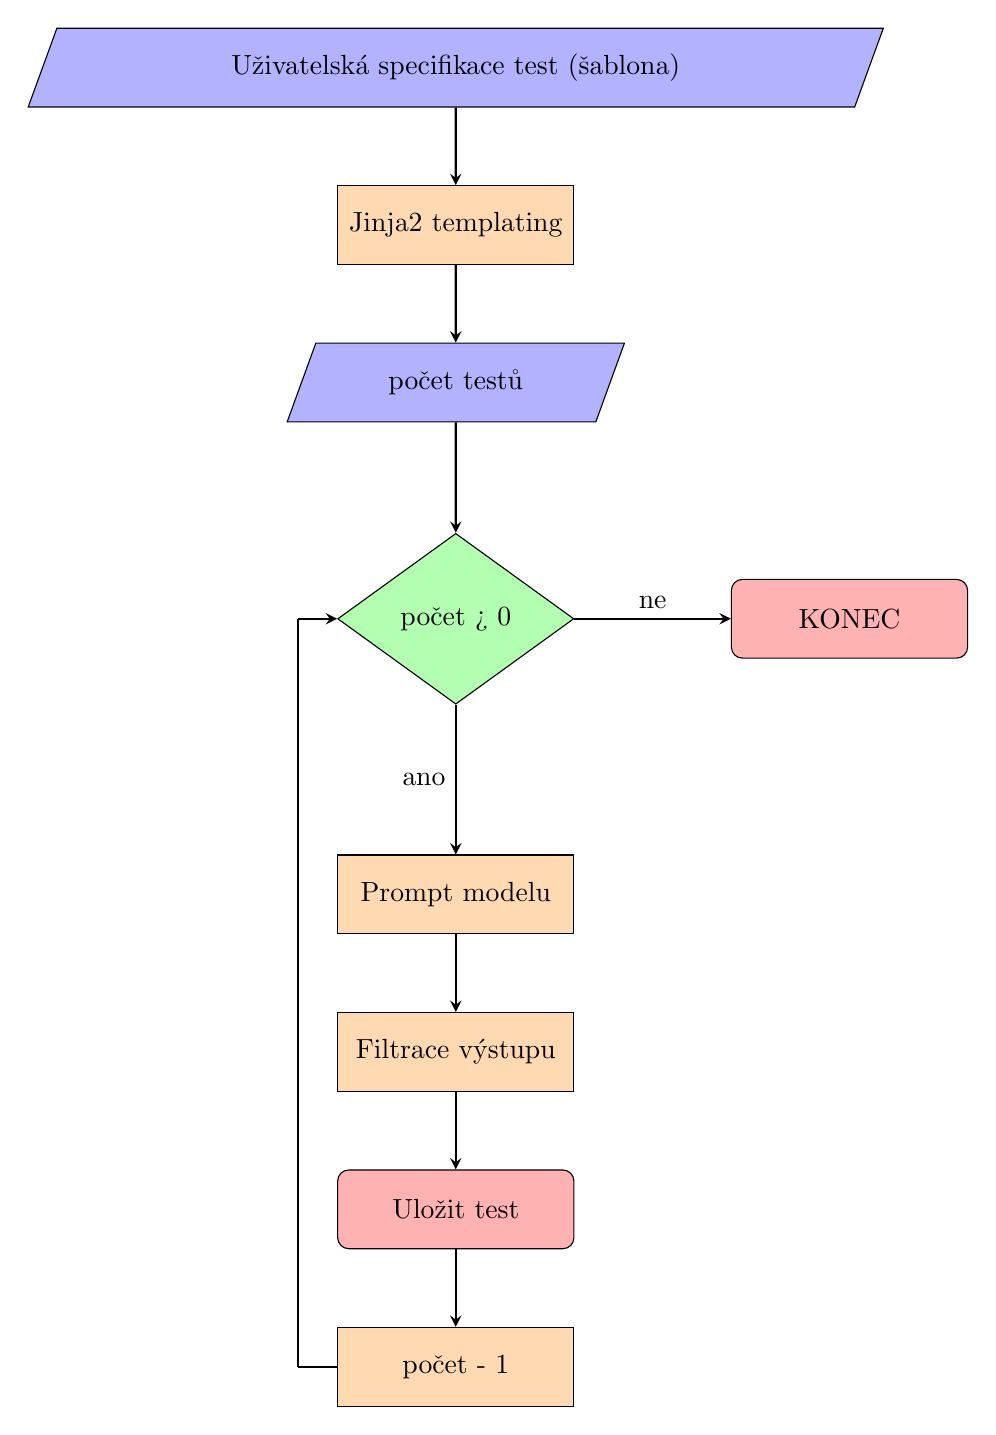
\begin{tikzpicture}[node distance=2cm]
                \node (start) [io] {Uživatelská specifikace test (šablona)};
                \node (in1) [process, below of=start] {Jinja2 templating};
                \node (in2) [io, below of=in1] {počet testů};
                \node (dec1) [decision, below of=in2, yshift=-1cm] {počet > 0};
                \node (pro1) [process, below of=dec1, yshift=-1.5cm] {Prompt modelu};
                \node (pro2) [process, below of=pro1] {Filtrace výstupu};
                \node (out1) [startstop, below of=pro2] {Uložit test};
                \node (procCount) [process, below of=out1] {počet - 1};
                \node (stop) [startstop, right of=dec1, xshift=3cm] {KONEC};
                \coordinate [left of=procCount] (lc);
                \coordinate [left of=dec1] (lif);

                \draw [arrow] (start) -- (in1);
                \draw [arrow] (in1) -- (in2);
                \draw [arrow] (in2) -- (dec1);
                \draw [arrow] (dec1) -- node[anchor=east] {ano} (pro1);
                \draw [arrow] (pro1) -- (pro2);
                \draw [arrow] (pro2) -- (out1);
                \draw [arrow] (out1) -- (procCount);
                \draw [arrow] (dec1) -- node[anchor=south] {ne} (stop);
                \draw [arrow] (procCount) -- (lc) (lc) -- (lif) (lif) -- (dec1);
            \end{tikzpicture}
            \centering
            \caption{Zjednodušené schema algoritmu pro dotazování jazykového modelu při generování testu.}
            \label{fig:llm_query_algo}
        \end{figure}

        \setuxprompt{milan}{dp/program}
        \begin{console}{Ukázka volání generace testu dle šablony \label{con:generation}}
`\uxprompt`python3 test.py -i spec-4 --count 10
        \end{console}

        Finální podoba promptu je poté skrze \textit{konektor} pro příslušné \Gls{llm} (například zmíněná \textit{OpenAI} knihovna, \textit{HTTP} dotaz či jiný druh konektoru) předána jako dotaz modelu. Společně s ním je i modelům předán v rámci těchto konektorů i \textit{systémový prompt}. V případě, že se je aktivní vstupní příznak programu \verb|--manual|, systémový prompt se přidá před vyrenderovaný prompt a tento spojený text je zkopírován do \textit{schránky}. Program načítá systémový prompt ze souboru \verb|templates/system.txt|. Jeho znění (viz výpis \ref{lst:system_prompt_used}) vychází poažadavků a nedostatků, které byli při testovacím generování zpozorovány.

        \begin{code}{text}{Použitý systémový prompt \label{lst:system_prompt_used}}
You're an intelligent programming assistant. You write Robot Framework scenarios and scripts using the Selenium Library. Insert delays between steps. Output code only, no text around. Use Chrome as browser. Locate elements using XPath. Close browser between scenarios.
        \end{code}

        \begin{code}{shell}{Ukázka ".env" souboru \label{lst:dot_env}}
API_URL="https://api.mistral.ai/v1"
API_KEY="Zca6nB87qmijn4"
API_MODEL="mistral-large-latest"

MAX_TOKENS=3000
DEVICE="mps"
        \end{code}

        I přes důraz na nutnost pouze \textit{programového} výstupu v rámci systémového promptu, mají modely tendeci tuto podmínku ignorovat a generovat text okolo kódu. Protože jsou modely naučené tak, aby jejich výstup byl text v \textbf{Markdown} formátu, obsahují i značky se začátkem kódového bloku a značením jazyka, ale také prvky jako odrážky, apod. Tyto prvky se pak objevují i ve výstupech, kde je požadován pouze \textit{čistý text} (jako například v ukázce \ref{lst:text_around}). V našem případě je toto chování nevhodné, protože vyžadujeme na výstupu pouze \textit{kód testu}. Díky struktuře \textit{Markdown} formátování však lze lze kód z tohoto výstupu jednoduše vyparsovat. Toto parsování má právě na starosti funkce \textit{filtrování výstupu} ve schematu \ref{fig:llm_query_algo}. V rámci programu byla implementována tak, že ze vstupního textu vyjme kód v prvním nalezeném kódovém bloku, označeného pomocí znaků \verb|```|. Pokud blok nenajde, vrátí původní text bez změny (předpokládá, že model se držel systémového promptu). V případě více kódových bloků přítomných ve výstupu, kdy požadovaný kód nebude v prvním z bloků, dojde k nesprávnému parsování, avšak jedná se o očekávaný případ, protože detekce správného kódu je \texti{netriviální} a zároveň \textit{subjektivní} problematika.

        \begin{code}{robotframework}{Výstup modelu s nadbytečným textem. \label{lst:text_around}}
Here's a Robot Framework scenario that follows the recorded JSON steps for interacting with the web page, and then performs the checks as specified:

```robotframework
*** Settings ***
Library           SeleniumLibrary

*** Variables ***
${URL}            http://localhost:4680/tbuis/index.jsp
${USERNAME}       lazy
${PASSWORD}       pass
${BROWSER}        Chrome

*** Test Cases ***
Open and Verify Webpage Content
...
```

In this Robot Framework script, I've incorporated commands that:
- Open the specified page and set the viewport size.
- Perform the login process using the provided username and password.
- Navigate to the "List of All Teachers" section.
- Check for the presence of specified names on the page.
- Validate the text content of specific table cells related to the teachers' courses.
Adjust the locators (xpath) as necessary to match the exact structure and identifiers used in your application's HTML.
        \end{code}

        Vyfiltrovaný výstupní text modelu je poté zapsán do souboru ve výstupní složce nazvané \verb|generated|, nacházející se v kořenové složce programu. Test je uložen s názvem ve formátu \verb|{nazev-vstupu}-{cislo-varianty}.robot| jakožto \textit{RobotFramework} soubor. První část tohoto názvu souhlasí s názvem \textit{promptové šablony}, pro kterou uživatel vytváří testy. Druhá část poté čísluje vygenerované varianty. Pokud již ve výstupní složce existuje vygenerovaný test pro danou specifikaci, program nové variantě přiřadí číslo o \(1\) vyšší, tedy pokračuje v číselné řadě. Názvy vygenerovaných testů jsou postupně vypisovány do konzole. Od uživatele je očekáváno, že vygenerované testy ve výstupní složce zkontroluje a ověří, že obsahují validní (\textit{např. obsahuje text, připomínající RobotFramework test}). Je zde totiž stále možnost, že model nevygenerovat žádný kód a vypsat pouze text nebo \textit{filtrace} neproběhla validně. Tento krok by v ideálním případě bylo možné automatizovat za pomocí \textit{analyzátoru} pro \textit{RobotFramework}, který se nachází v rámci \Gls{lsp} pro \textit{RobotFramework} \verb|rebotframework-lsp| nachází. Bohužel však neumí validovat zápis pro knihovnu \verb|SeleniumLibrary|, která je v rámci systémového promptu vyžadována a očekávána, že bude přítomná ve vygenerovaném testu.

\chapter{Spuštění testů}
 
    V této kapitole je diskutováno spuštění vygenerovaných testů a jde o implementaci kroku popisovaného v návrhu (\ref{sec:proposal}). Samotnému spuštění vybrané sady testů musí nejdříve předcházet nasazení testovaného softwaru, pro které zde byla vytvořena automatizovaná orchestrace využívající technologii \textit{Docker}. Dále bylo také potřeba spustit samotné testy na vybraných varinatách testované aplikace. I o toto spuštění se stará orchestrační software. Popsána zde je také \emph{konfigurace}, která je pro jednotlivé kroky potřeba, a jak jsou ukládány výsledky testů společně s jejich formátem.

    \section{Spuštění testovaného programu a jeho orchestrace}

    %TODO tady nějaké citace
    Testovaný program \textit{TbUIS} (popsaný v sekci \ref{sec:test_program}) je distribuován jakožto \verb|.WAR| soubory, tedy komprimovaný webový archiv jazyka Java, spustitelný jakožto \gls{servlet}. Z dokumentace projektu a předchozích diplomových prací vyplývá, že pro nasatení je určený aplikační server \textit{Tomcat} verze \(7\) až \(9\). S vyššími verzemi není aplikace kompatibilní. Každá varianta aplikace (\textit{poruchové klony}) je distribuována jako samostatný \textit{WAR} soubor. Pro spuštění konkrétní varinaty a spuštění vygenerovaných testů na této variantě bylo nutné vytvořit \textit{automatizované nasazení} aplikace \textit{TbUIS}. Pro nasazení je nutné brát v úvahu nejen samotnou webovou aplikaci, ale i její závislost, kterou je \textit{databáze} MySQL (resp. MariaDB), která musí být inicializována dodaným skriptem.

    \subsection{Vytvoření kompozice} \label{sec:composition}
    Pro účely \textit{automatizovaného nasazení} byla zvolena technologie \textit{Docker}, tedy \textit{kontejnerové} řešení s možností vytvářet obrazy a kompozice. Právě kompozice je vhodným nástrojem pro jednoduché \textit{lokální} nasazení aplikace \textit{TbUIS}, protože potřebujeme 2 samostatné kontejnery; první s \textit{aplikačním servervem} a druhý s \textit{databází}.

    Před samotnou integrací je nutné v každé z variant aplikace (\textit{WAR} soubory) změnit \textit{adresu} databáze. Docker kompozice umoňují přidělit jednotlivým kontejnerům názvy, kterými lze v rámci interní DNS tyto kontejnery adresovat. V rámci archivů bylo nutné modifikovat adresu v souborech \textit{WEB-INF/classes/META-INF/persistence.xml} a \textit{WEB-INF/classes/applicationContext.xml}. Pro zjednodušení vlastního nasazení jsou modifikované webové archivy součástí repozitáře této práce. Pro kontejner \textit{databáze} byl zvolen název \verb|tbuis-db|. Veškeré potřebné soubory pro spuštění testovaného programu se nachází ve složce \verb|tbuis| v rámci programové složky.

    K vytvoření \textit{kompozice} je potřeba mít také obrazy, ze kterých se budou vytvářet kontejnery. Zatímco pro databázi stačí \textit{MariaDB} kontejner z veřejného repozitáře, tak pro aplikační server je potřeba vytořit vlastní obraz, který bude vycházet z obrazu pro \textit{Tomcat} aplikační server, ale vždy do něj budou nahrána data jiné varianty aplikace. Pro vytoření obrazu byl do složky přidán \textit{Dockerfile} sloužící k jeho sestavení. Obsah tohoto souboru lze vidět v ukázce \ref{lst:dockerfile}. Skript přebírá cestu k \textit{WAR} souboru za pomocí argumentu a ten poté vkládá do obrazu na předem definovanou cestu a s definovaným názvem. V rámci Tomcat kontejneru slouží právě složka \verb|webapps| pro servlety a jejich název udává cestu, které v rámci HTTP dotazů jsou dostupné. Pro zvolený název \verb|tbuis| tedy odpovídá cesta \verb|/tbuis|.

    \begin{code}{dockerfile}{Dockerfile pro sestavení obrazu varianty aplikačního serveru. \label{lst:dockerfile}}
FROM tomcat:9.0
ARG WAR_FILE
COPY ${WAR_FILE} /usr/local/tomcat/webapps/tbuis.war
    \end{code}

    Obraz z \textit{Dockerfile} lze vytvořit samostatně, ale také lze jeho sestavení zavolat při vytváření kompozice. To se provádí nástrojem \textit{Docker Compose}. Defaultní název souboru, který příkaz pro vytváření kompozice \verb|docker-compose up| využívá je \verb|docker-compose.yml|. Takovýto defaultní soubor je vytvořen v podsložce programu \verb|tbuis| (jeho obsah se nachází v ukázce \ref{lst:docker-compose}). Jak přípona souboru naznačuje, jedná se o textový soubor ve formátu \textit{YAML}. V rámci něj definujeme dvojici služeb potřebných pro nasazení aplikace. Službou v kompozici je myšlen kontejner. Při vytváření služby lze definovat i její \textit{proměnné prostředí}, \textit{porty} a jejich předávání, \textit{připojené} složky, \textit{sítě} a další vlastnosti běžně nastavované pro kontejner. Pro \textit{databázi} je potřeba předat port \(3306\), ale také připojit složku s inicializačními skripty (v našem případě dostupná ve stejné složce jako kompoziční soubor). V ní se nachází soubor \verb|init-db.sql|, který obsahuje příkazy pro vytvoření databáze s daným názvem a uživatele, za kterého se aplikační server připojuje. U služby aplikačního serveru je potřeba sestavit obraz. Pro toto sestavení využíváme vytvořený Dockerfile, nacházející se ve stejné složce. Také je potřeba předat argument s cestou pro \textit{WAR} soubor, který bude do serveru nahraný. Pro přístup do webového rozhraní aplikace z venčí kompozice byl zvolen port \(4680\) předaný z defaultního portu \(8080\), který aplikace používá. Tento port bude sloužit vygenerovaným testům pro přístup. V případě potřeby může uživatel tento port změnit dle svých požadavků. Oba kontejnery jsou také připojeny do stejné \textit{virtuální sítě}, který zajišťuje komunikaci mezi nimi. 

    \begin{code}{dockerfile}{Docker Compose soubor pro sestavení kompozice \label{lst:docker-compose}}
version: '3.8'

services: 

  db:
    image: mariadb
    container_name: tbuis-db
    environment: 
      MARIADB_ROOT_PASSWORD: testtest
    ports:
      - "3306:3306"
    volumes: 
      - ./db:/docker-entrypoint-initdb.d/
    networks:
      - tbuis

  tomcat:
    build:
      context: .
      args:
        WAR_FILE: ${WAR_FILE_PATH}
    container_name: tbuis-tomcat
    depends_on:
      - db
    ports:
      - "4680:8080"
    networks:
      - tbuis

networks: 
  tbuis:
    driver: bridge
    \end{code}

    Pro vytvoření a spuštění této kompozice je potřeba zavolat příkaz z ukázky \ref{lst:compose_up_command}, kde příkaz \verb|up| vyjadřuje právě \textit{vytvoření} kompozice. Pro povolení sestavení obrazu v rámci vytváření kompozice, je také potřeba přidat argument \verb|--build|. Aby se kontejnery spustili na pozadí a ne v terminálu, je také vyžadován argument \verb|-d|. Zároveň z důvodu, abychom nástroj \verb|docker-compose| nemuseli volat pouze ze složky, ve které se kompoziční soubor nachází, lze také přidat argument \verb|-f| a hodnotou cesty ke konfiguračnímu souboru. Před příkazem je také vyexportována proměnná prostředí \verb|WAR_FILE_PATH|, která určuje variantu serverletu, který bude nasazen do webové aplikace. Jedná se o cestu relativní vůči \textit{docker compose} souboru. V případě nutnosti \textit{smazat} kompozici, je také možnost zavolat příkaz \verb|docker-compose down| (viz ukázka \ref{lst:compose_down_command}). Protože při vytváření kompozic byli sestaveny i obrazy, které mohou na počítači zbírat nemalé místo, je také k příkazu přidán argument \verb|--rmi all|, který mimo kotejnerů vytvořených kompozicí smaže i nevyužívané obrazy.

    \setuxprompt{milan}{dp/program}
    \begin{console}{Vytvoření Docker kompozice z připravené konfigurace \label{lst:compose_up_command}}
`\uxprompt`WAR_FILE_PATH=./defect-00_free.war docker-compose -f tbuis/docker-compose.yml up -d --build
    \end{console}

    \begin{console}{Smazání Docker kompozice společně s vytvořenými obrazy \label{lst:compose_down_command}}
`\uxprompt`docker-compose -f tbuis/docker-compose.yml down --rmi all
    \end{console}

    \subsection{Orchestrace a automatizace nasazení} \label{sec:orchestration}

    Výše vypsané příkazy automatizují nasazení jedné z variant webové aplikace. Namísto jejich manuálního volání však bude tento úkon provádět orchestrační program \verb|test.py| v režimu \verb|-r| (\textit{run}). Příklad takového volání se nachází v ukázce \ref{lst:run_mode}. Samotná orchestrace spuštění vygenerovaných testů spočívá v tom, že program nasadí jednu z požadovaných variant aplikace, poté postupně spustí jednotlivé testy vyhovující zadanému kritériu v rámci hodnoty pro argument režimu \verb|-r|. Po dokončení všech testů je načtena další z požadovaných verzí aplikace pro nasazení a otestování. Zvolené testy jsou tedy spuštěny na všech vybraných variantách (orchestrace nastíněna v obr. \ref{fig:orchestration}). Po dokončení testování je poté vytvořená kompozice společně se všemi jejími sestavenými a staženými obrazy smazána. K těmto úkonům je využit právě nástroj \textit{Docker} a \textit{Docker Compose}, popsané v sekci \ref{sec:composition}. Mezi jednotlivými testy spouštěnými na jedné z variant aplikace je také potřebna provést \textit{obnovení databáze}, protože některé z testovacích scénářů databázi modifikují (viz tabulky \ref{tab:specs_1} a \ref{tab:specs_2}). Pro toto obnovení nabízí aplikace \textit{HTTP} endpoint nebo tlačítko na úvodní stránce. Pro zjednodušení byl mezi statické soubory přidán RobotFramework scénář, který na toto tlačítko na úvodní stránce klikne.

    \begin{console}{Spuštění orchestračního programu v režimu spouštění testů \label{lst:run_mode}}
`\uxprompt`python3 test.py -r "codellama/spec-*" --name "codellama-runs"
    \end{console}

    \begin{figure}
        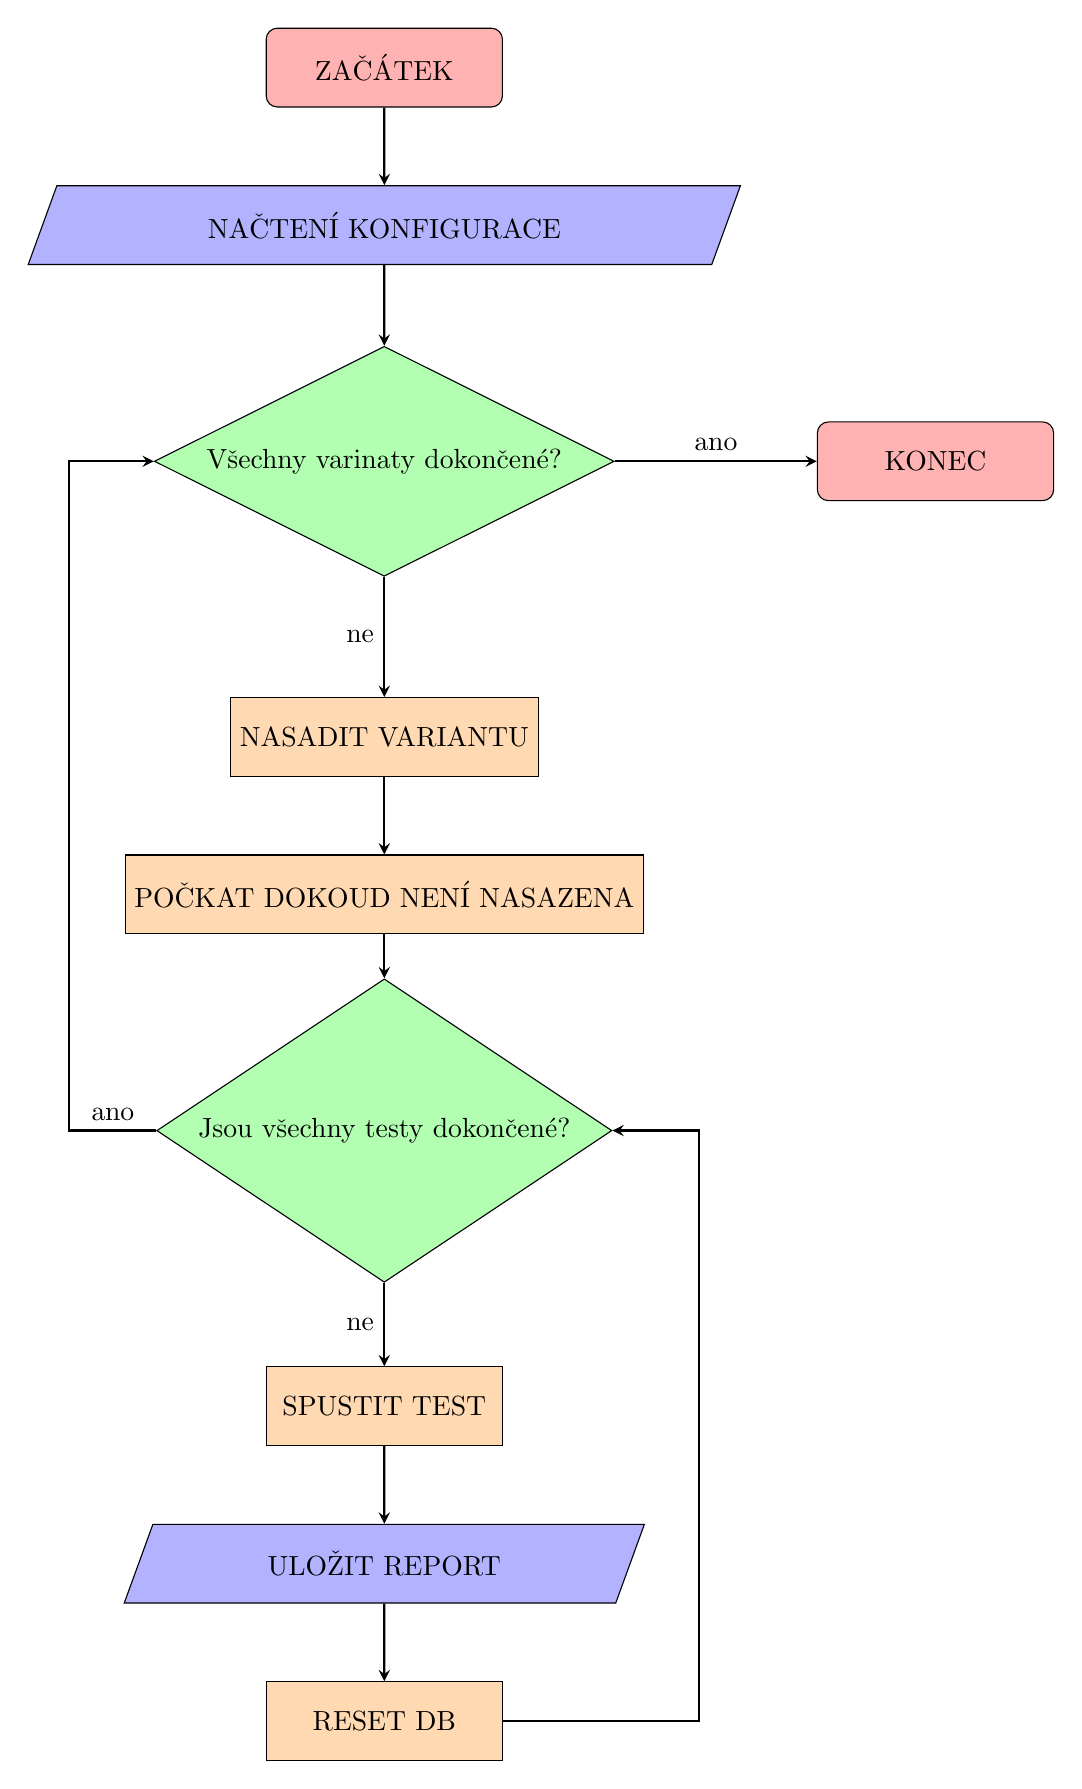
\begin{tikzpicture}[node distance=2cm]
            \node (start) [startstop] {ZAČÁTEK};
            \node (loadConfig) [io, below of=start] {NAČTENÍ KONFIGURACE};
            \node (decision1) [decision, aspect=2, below of=loadConfig, yshift=-1cm] {Všechny varinaty dokončené?};
            \node (end) [startstop, right of=decision1, xshift=5cm] {KONEC};
            \node (deployVariant) [process, below of=decision1, yshift=-1.5cm] {NASADIT VARIANTU};
            \node (waitDeploy) [process, below of=deployVariant] {POČKAT DOKOUD NENÍ NASAZENA};
            \node (decision2) [decision, aspect=1.5, below of=waitDeploy, yshift=-1cm] {Jsou všechny testy dokončené?};
            \node (runTest) [process, below of=decision2, yshift=-1.5cm] {SPUSTIT TEST};
            \node (saveReport) [io, below of=runTest] {ULOŽIT REPORT};
            \node (resetDB) [process, below of=saveReport] {RESET DB};
            \coordinate [left of=decision1, xshift=-2cm] (ld1);
            \coordinate [left of=decision2, xshift=-2cm] (ld2);
            \coordinate [right of=resetDB, xshift=2cm] (rdb);
            \coordinate [right of=decision2, xshift=2cm] (rd2);

            \draw [arrow] (start) -- (loadConfig);
            \draw [arrow] (loadConfig) -- (decision1);
            \draw [arrow] (decision1) -- node[anchor=east] {ne} (deployVariant);
            \draw [arrow] (deployVariant) -- (waitDeploy);
            \draw [arrow] (waitDeploy) -- (decision2);
            \draw [arrow] (decision2) -- node[anchor=east] {ne} (runTest);
            \draw [arrow] (runTest) -- (saveReport);
            \draw [arrow] (saveReport) -- (resetDB);
            \draw [arrow] (decision1.east) -- node[anchor=south] {ano} (end);
            \draw [arrow] (decision2.west) -- node[anchor=south] {ano} (ld2) -- (ld1) -- (decision1.west);
            \draw [arrow] (resetDB) -- (rdb) -- (rd2) -- (decision2.east);
        \end{tikzpicture}
        \centering
        \caption{Znázornění orchestrace spouštění testů}
        \label{fig:orchestration}
    \end{figure}

    Spuštící režim programu nabízí možnost hned několika argumentů a jejich hodnot. Požadovaná hodnota je zde pro \textit{režimový} argument \verb|-r|, která musí obsahovat název nebo vzor názvu testů, které se v rámci složky \textit{generated} mají spustit. Pro přehlednost si uživatel může ve výstupní složce testů rozdělovat vygenerované testy do podsložek, případně držet vhodnou konvenci pro jejich označení. Hodnota pro vzor názvu testů může být jakýkoliv validní \textit{UNIX wildcard} pro označení souborů. Příklad použití takovéto \textit{wildcard} lze vidět v ukázce \ref{lst:run_mode}, kde se spouští testy (resp. soubory) z podsložky \verb|codellama|, které vyhovují vzoru \verb|spec-*|, což znamená všechny soubory začínající řetězcem "spec-"  v této podsložce. Tento přístup pro zvolení cesty a souborů umožňuje nejen právě dělit výstupní složku testů na podsložky, ale také uživateli spustit jen konkrétní vybrané testy. Spuštění pouze omezené množiny testů je ukázáno ve výpisu \ref{lst:run_mode_2}, kde uživatel požaduje spustit testy vyhovující specifikaci \(1\), \(4\) a \(6\) ve všech jejich varintách (značení vygenerovaných testů popsáno v sekci \ref{sec:llm_requests}) ve složce "openai-gpt-4" (tedy například testy vygenerované modelem GPT-4 od OpenAI). Hodnoty pro tento argument je vhodné psát v \emph{uvozovkách}.

    \begin{console}{Alternativní volání režimu spuštění testů \label{lst:run_mode_2}}
`\uxprompt`python3 test.py -r "openai-gpt-4/spec-{1,4,6}-*" --cont_count 2 --name "gpt-4 test runs"
    \end{console}

    Další argumenty pro \textit{spouštěcí} řežim jsou již \emph{nepovinné}, avšak alespoň argument \verb|--name| je doporučený. Tímto argumentem lze nastavit jméno aktuálního běhu testů, kterým lze poté jednoduše identifikovat s ním související výsledky. Samotné výsledky, jejich ukládání a struktura jsou vysvětleny v následující sekci kapitoly. Pro hodnotu tohoto argumentu je také doporučené využít uvozovky (ukázkové volání jak v příkladu \ref{lst:run_mode} a \ref{lst:run_mode_2}). Pro zkušební běhy testů lze také využít argument \verb|--cont_count|, jehož hodnota omezí počet volaných variant aplikace, dostupných z \textit{konfigurace} (číselná hodnota vyšší než \(0\)).

    Samotný běh aplikace, testů a jejich případného vyhodnocení neovlivňují pouze \emph{argumenty}, ale také komplexnější \emph{konfigurace}, která se nachází v rámci konfiguračního souboru \verb|configuration.py|. Jednotlivé varinaty aplikace, které se budou spouštět v rámci běhu lze zvolit tak, že se názvy jejich \textit{WAR} souborů ze složky \verb|tbuis| přidají do pole \verb|RUN_CONTAINERS| v rámci konfigurace. 

    \begin{code}{python}{Zjednodušená ukázka konfiguračního souboru \label{lst:configuration}}
RUN_CONTAINERS = [
    "defect-00_free.war",
    "defect-02-C0.H0.M0.L1_S_S_03.war",
    "defect-04-C0.H0.M0.L1_S_S_04.war",
    ...
    "defect-26-C1.H0.M0.L0_T_S_01.war",
    "defect-27-C1.H0.M0.L0_U_D_01.war",
    "defect-28-C2.H2.M1.L0_M_CR.war"
]

POSITIVE_FAILS = {
    "1": ["defect-02-C0.H0.M0.L1_S_S_03.war"],
    "4": ["defect-04-C0.H0.M0.L1_S_S_04.war", "defect-19-C0.H1.M0.L0_S_S_10.war", "defect-25-C1.H0.M0.L0_S_S_01.war", "defect-26-C1.H0.M0.L0_T_S_01.war", "defect-28-C2.H2.M1.L0_M_CR.war"],
    "6": ["defect-25-C1.H0.M0.L0_S_S_01.war", "defect-26-C1.H0.M0.L0_T_S_01.war", "defect-28-C2.H2.M1.L0_M_CR.war"],
    ...
}\end{code}
    
    \section{Ukládání výsledků}
    Při spuštění testu vyváří \textit{RobotFramework} hned několik výstupních souborů, mezi kterými je i \textit{report} jakožto soubor \verb|output.xml|. V rámci něj se nacházejí veškteré klíčové informace o běhu scénáře. Konkrétně jde o \textit{log} provedených úkonů, \textit{výsledky} jednotlivých testovacích případů a také případné \textit{errory} (kritické chyby, kvůli kterým nelze vygenerovaný test ani spustit). Protože tento výstup obsahuje spoustu redundantních informací, je v rámci programu zpracován a uložen na 2 samostatná místa. Z původního výstupu jsou vyjmuty hodnoty: \textit{počet úspěšných}, \textit{neúspěšných} a \textit{chybových} testovacích případů pro každý ze spuštěných testovacích scénářů. Pro ten je vždy také vyhodnocen koncový stav (\textit{FAIL, PASS} nebo \textit{ERROR}). Protože \textit{RobotFramework} nerozlišuje mezi testem, který \emph{selhal} a testem, který nešel spustit nebo při jeho běhu došlo k chybě nesouvisející se scénářem, bylo potřena toto rozlišení implementovat na bázi přítomných \textit{errorů} (jakožto značek) v rámci výstupního souboru. 

    Pro označení výsledku testu (dále také jako \emph{report}) je využito \textit{časové razítko} doby spuštění série testů ve formátu \verb|YYYYMMDDhhmmss| společně s vybraným názvem v rámci argumentu (popsáno v předchozí sekci \ref{sec:orchestration}) oddělěných znakem "-". V případě, že samostatný název běhu testů není uživatelem vybrán, zůstává pro plné označení reportu pouze časové razítko.

    Prvním z míst pro uložení výsledků je textový soubor uložený ve podsložce \verb|reports| v rámci kořenové složky programu. V rámci tohoto souboru jsou vykresleny textové tabulky, vykreslené pro každou nasazenou variantu aplikace (varianty jsou v rámci programu také označovány jako kontejnery, protože odpovídají kontejneru Dockeru). V rámci tabulky jsou pro každý spuštěný test vypsány výsledky jednotlivých sledovaných údajů a koncový výsledek testu. Ukázka tabulky je vyzobrazena na obr. \ref{fig:report_table}. Název tabulky odpovídá právě testovanému kontejneru (resp. varianty testu). Soubor report je pojmenovaný jeho celým názvem, jak bylo popsáno v předchozím odstavci.

    Ačkoliv tabulková reprezentace výsledků v textové podobě je jednoduchá pro uživatele a jeho čtení, tak již není vhodná pro strojové čtení a zpracování, proto jako druhá možnost pro uložení výsledů byla zvolena \textit{SQLite} databáze, resp. soubor \verb|report_db.sqlite| umístěný ve stejné podložce \verb|reports| jako textové reporty. Tento druh formátu byl zvolen z důvodu jeho jednoduchosti a široké podpoře napříč programovacími jazyky. V rámci této databáze je vytvořena tabulka "runs", která obsahuje řádky s hodnotami výsledků jednotlivých testovacích scénářů, podobně jako v případě tabulek textového reportu. Narozdíl od nich se zde pro veškeré údaje využívá jedna tabulka a mezi jednotlivými běhy jde rozlišit primárně dle jejich názvu. Ukázka tabulky je vyzobrazena na obr. \ref{fig:sqlite_report}. V rámci malé lokální databáze je poté možné data efektivně vyhledávat, filtrovat a nadále s nimi pracovat.
   
    \begin{figure}
        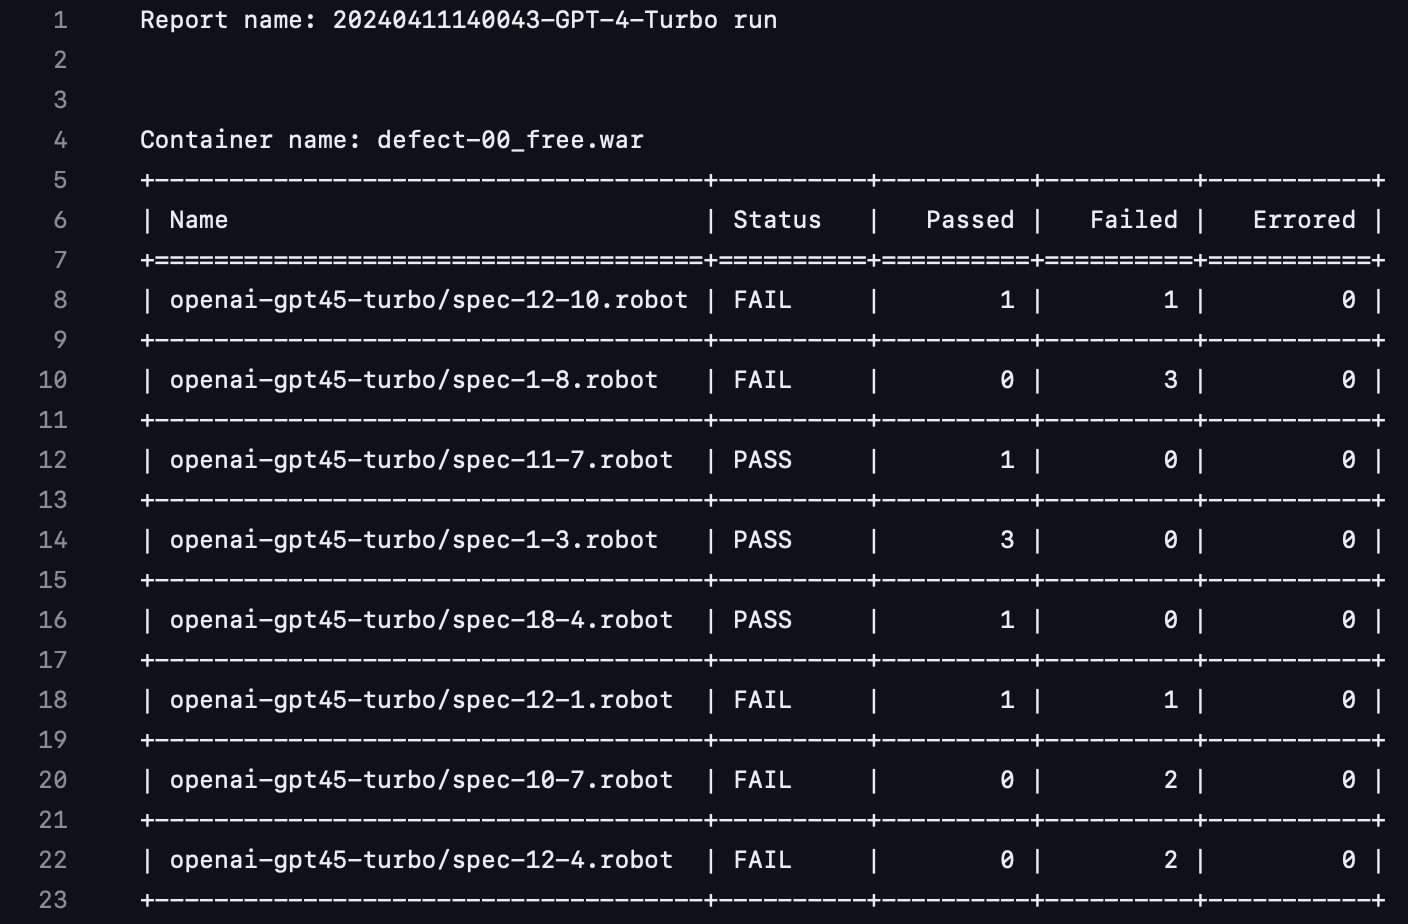
\includegraphics[width=0.8\textwidth]{pic/report_table.png}
        \centering
        \caption{Ukázka textové tabulky výsledků}
        \label{fig:report_table}
    \end{figure}

    \begin{figure}
        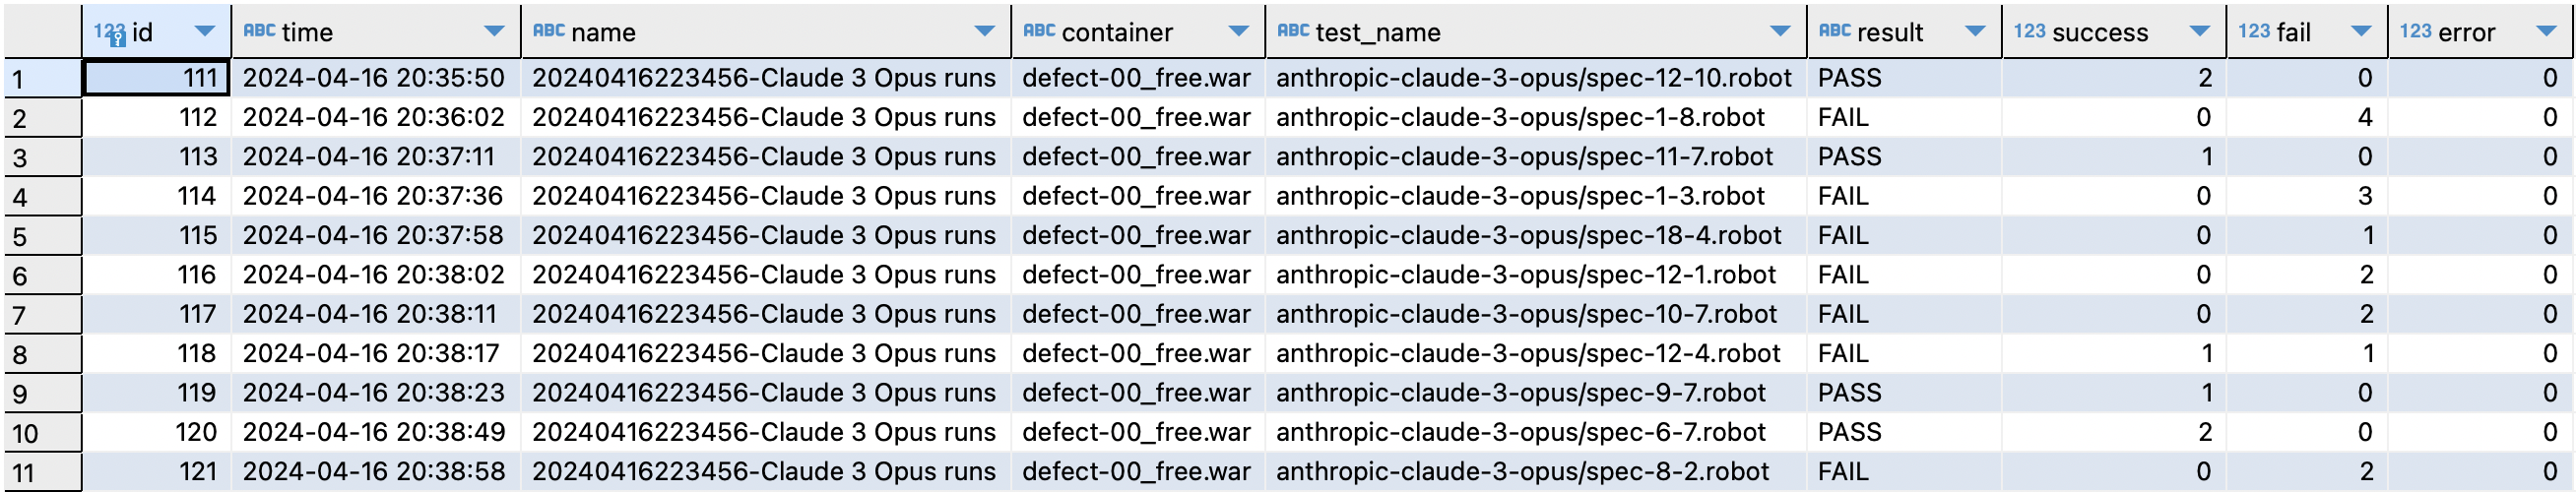
\includegraphics[width=\textwidth]{pic/sqlite_example.png}
        \centering
        \caption{Ukázka databázové tabulky výsledků}
        \label{fig:sqlite_report}
    \end{figure}

\chapter{Vyhodnocení výsledků}

    V rámci této kapitoly jsou \emph{analyzovány} výsledky testů, které byly pro účely této práce \textit{vygenerované a spuštěné} skrze metody popsané v předchozích kapitolách. Popsána je zde kompletní metodologie, která pro vyhodnocení výsledků byla využita a také jsou popsané tabulky výsledků. V rámci analýzy se budeme zaměřovat primárně na kvalitativní stránku vygenerovaného zdrojového kódu testů. V závěru kapitoly je také rychlé srovnání s lisky psanými testy, které jsou k testované aplikaci k dispozici a je diskutována i náročnost generování na zdroje (\textit{finance, čas, energie}).

    \section{Parametry pro spuštění} \label{sec:run_parameters}

    Vygenerované testy z kroku \ref{sec:test_generation} (konkrétně scénáře vypsané v tabulkách \ref{tab:specs_1} a \ref{tab:specs_2}) byly v rámci výstupní složky \verb|generated| rozděleny do podsložek s odpovídajícím názvem, ze kterého je patrné, jakým modelem (případně od jaké společnosti) byly vygenerovány. Možnost takového rozdělení byla popsán v sekci \ref{sec:orchestration}. Tyto vygenerové testy, využité k následnému testování poruchových klonů, jsou součástí programového repozitáře projektu. Do konfiguračního souboru byly přidány varianty aplikace dle tabulky \ref{tab:clones} (ukázka konfiguračního souboru ve výpisu \ref{lst:configuration}). Z tabulky scénářů také víme, pro které varianty testovacího programu také můžeme očekávat chybu v daném scénáři. Proto je do konfiguračního souboru přidáno i \textit{mapování}, které každému scénáři (označené pouze číslem) přiřazuje pole názvů \textit{WAR} souborů aplikace, ve kterých je chybovost očekávána. Na bázi tohoto mapování dále vyhodnocovací program určí správnost výsledku testu (tj. v případě očekávaného selhávání jde o správný výsledek). Tento program a použité metody jsou popsány v následující sekci.

    \begin{console}
`\uxprompt`ls -l generated
 15 milan  staff   480 May  5 09:59 .
 19 milan  staff   608 May  6 22:38 ..
102 milan  staff  3264 Apr 30 15:07 anthropic-claude-3-opus
102 milan  staff  3264 Apr 16 07:40 codellama
102 milan  staff  3264 May  4 09:45 gemini-1.5-pro
102 milan  staff  3264 May  3 18:52 local-llama3
102 milan  staff  3264 Apr 30 15:07 mistral-large
102 milan  staff  3264 May  5 11:05 mistral-v0.2
  3 milan  staff    96 May  5 09:59 openai-gpt35
102 milan  staff  3264 Apr 30 15:07 openai-gpt4
102 milan  staff  3264 May  3 18:52 openai-gpt4-turbo
102 milan  staff  3264 May  5 09:59 wizardcoder-python\end{console}
    
    \section{Metodologie vyhodnocení}

        Následující text v krátkosti popisuje, jaké statické metody a postupy jsou k vyhodnocení výsledků využity a na jakých předpokladech pro výstupy automatizovaného testování je vytvořený statistický nástroj postaven, případně jaké paramery od uživatele vyžaduje. Společně s metodou je vysvětlena i vizualitace a přidán je zde také důkaz o předpokladu pro pravá a případně falešná negativa, která jsou v rámci metody detekována. Hodnotit se bude, zda zaznamenané výstupní stavy testů odpovídají předpokladu.
        
        \subsection{Vyhodnocovací program} \label{sec:evaluation}

        Pro vyhodnocení výsledů byl do programové složky vytvořen program \verb|stats.py|, který jako první argument vyžaduje cestu s \verb|.sqlite| výstupnímu reportu hlavního programu v režimu běhu (viz sekce \ref{sec:orchestration}). Ukázkové volání programu je zobrazeno v ukázce \ref{lst:stats_call}. Tento report si uživatel může libovolně přesouvat v souborovém systému. Reporty vygenerované v rámci tohoto projektu a využité pro hodnocení modelů byly uloženy do podsložky \verb|results| kořenové složky repozitáře. Program má i další argumenty, které jsou jeho klíčovou součástí:
        \begin{itemize}
            \item \verb|-t [nadpis]| - Nastaví nadpis nad tabulkou (název modelu).
            \item \verb|-e [nazev_souboru]| - Vyexportuje soubor do PDF. Hodnotou je název výstupního PDF souboru (s příponou).
        \end{itemize}
        Pro každý test je vyhodnoceno, kolik z jeho vygenerovaných variant pro každou variantu testovacího programu skončilo s \textit{očekávaným výsledkem}. Tím je zde myšleno, že test prošel úspěšně na variantách aplikace, kde se nevyskytuje chyba a je tak očekáván bezchybný průchod, a že test selhal v na takových variantách, kde je definováno specifikací (diskutováno v sekci \ref{sec:run_parameters}), že by selhat měl. Chybový test je vždy považován za \textit{neočekávaný výsledek}. Při takto naivním přístupu by však jako \emph{očekávané} byly označovány i testy (resp. jejich vygenerované varianty) chybující i v případě nasazených variant aplikace bez konkrétní testované chyby (tedy falešná negativa). Z důvodu, aby takové testy nezkreslovali výsledky, bylo přistoupeno ke kroku jejich vyřazení a následnému ignorování při vyhodnocování výsledků.

        Pro odhalení falešných negativ budeme využívat předpokladu výsledku na \emph{neporuchové} variantě aplikace, že varianta testu skončí úspěšně. V případě, kdy dojde k jejímu selhání nebo skončí chybou, je taková testová varinta ignorována při vyhodnocení výsledků testů na všech poruchových kontejnerech, protože se předpokládá, že takový test není schopen správně odhadit chybu aplikace, protože by chybový stav hlásil vždy. Počet ignorovaných variant od každého testu je zobrazen ve spodní řádce tabulky výsledků (více v následující sekci \ref{sec:plot_legend}).

        \begin{console}{Volání programu pro vyhodnocení dat. \label{lst:stats_call}}
`\uxprompt`python3 stats.py ../results/claude-3-opus-run.sqlite -t "Claude 3 Opus" -e claude-results.pdf
        \end{console}

        \subsection{Legenda tabulek} \label{sec:plot_legend}

        Výstupem vyhodnocení výsledků je tabulka (jako příklad poslouží výstup v obr. \ref{fig:res:gpt-4}), jejíž řádky reprezentují testované \textit{varianty aplikace} (v tabulce označované jako \emph{container}) a jednotlivé sloupce představují konkrétní test (dle specifikace), který byl spouštěn. Jednotlivé buňky poté obsahují informaci o počtu variant daného testu, které vyhovují předpokládanému výsledku pro danou variantu aplikace. Tyto hodnoty jsou po vyfiltrování, které se vždy děje dle první řádky od shora (v našem označení jde o variantu \verb|defect-00_free.war|). Tento přístup byl popsán v předchozí sekci \ref{sec:evaluation}. Ve spodním řádku tabulky je také vyznačeno, kolik variant daného testu bylo \emph{ignorováno}. Celá tabulka zároveň funguje jako \textit{tepelná mapa} a je tedy nejen číselně, ale i barevně vyznačeno, jaký test má pro kterou variantu aplikace nejvyšší míru úspěšnosti (shody s předpokládaným výsledkem). Barevná škála a její odpovídají hodnoty se nachází po pravé straně tabulky.

        \subsection{Předpoklady}

        %TODO Někam pak taky ověření, že výběr true negatives je správný - asi sem
        %TODO Dopsat a asi ty konkrítní výsledky dát do přílohy 

    \section{Výsledky pro jednotlivé modely}

        Tato sekce je rozdělena do kategorií dle původního vývojáře modelu, ve kterých jsou poté postupně popisovány výsledky jednotlivých modelů (tabulky) a je analyzována jejich struktura a kvalita výstupního kódu. V rámci kvality se zaměřujeme jak na validní tak chybné úsudky, které model predikoval.
    
        \subsection{OpenAI} \label{sec:res:openai}

            \begin{figure}
                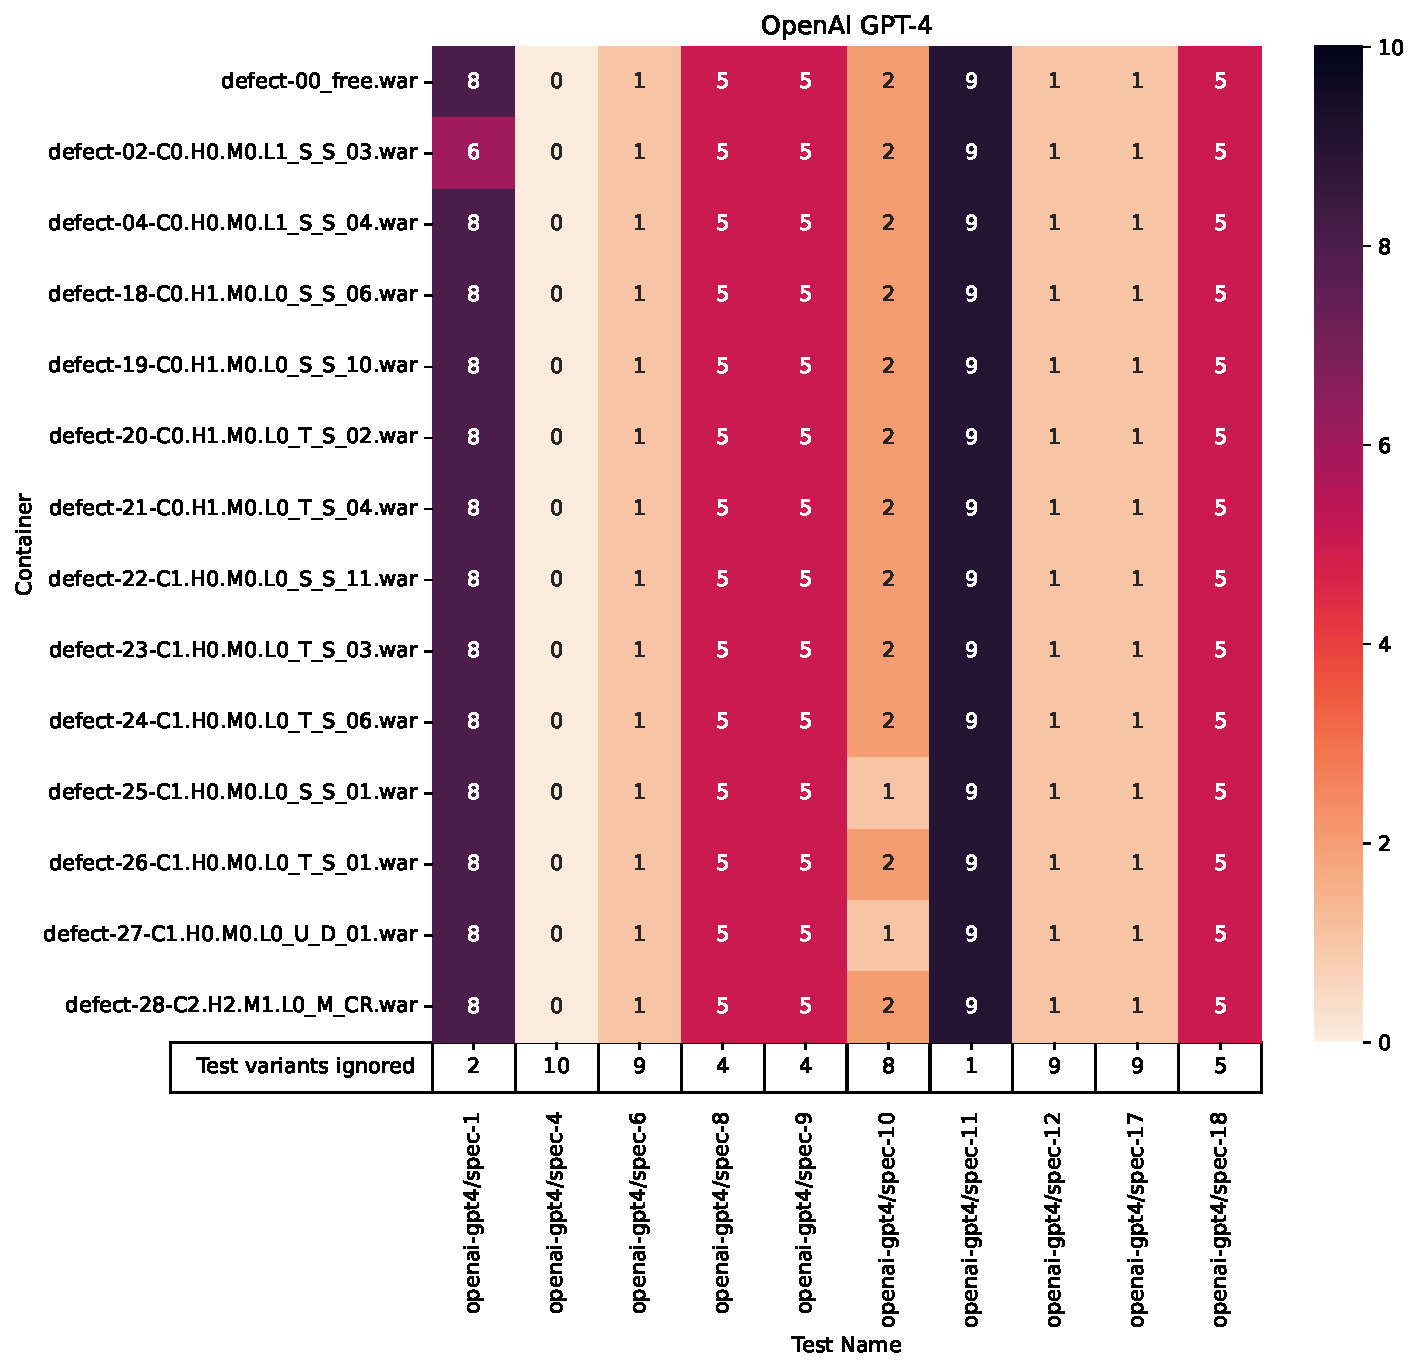
\includegraphics[width=\textwidth]{pic/gpt-4-results.pdf}
                \caption{Výsledky pro model GPT-4}
                \label{fig:res:gpt-4}
            \end{figure}

            Model \textbf{GPT-4} od společnosti OpenAI dokázal pro většinu \textit{testových případů} vygenerovat minimálně \emph{jeden} test podávající pro všechny testované varianty aplikace očekávaný výsledek. Výsledky zobrazené v obr. \ref{fig:res:gpt-4}. Jediný test, pro který model \textit{GPT-4} nebyl schopen vygenerovat ani jednu variantu testu, která by podala očekávaný výsledek, pro specifikaci 4 (viz \ref{tab:specs_1}). Tento konkrétní testový případ popisuje odhlášení studenta ze zkoušky a následnou kontrolu učitelem, zda je seznam studentů, přihlášených na zkoušce, prázdný. Každá z vygenerovaných variant hlásila pro tento případ poruchu i na klonech, které by ji pro tento případ neměli vykazovat. Primárním probléme ve vygenerovaném kódu zde byla nesprávná identifikace prvků, které mají být stisknuty nebo měla být detekována jejich hodnota následně srovnána s očekávanou. V případě studenta častokrát nedochází k úspěšnému odhlášení ze zkoušky, což vede i k následnému selhání \textit{test casu} ze strany učitele. Na této straně zároveň docházelo k nesprávnému výběru předmětu z rozbalovacího seznamu. Například v obr. \ref{fig:wrong_subject_select}, kde správně má být zvolený předmět \uv{Database Systems}.

            \begin{figure}
                
\includegraphics[width=0.8\textwidth]{pic/wrong_subject_select.png}
                \centering
                \caption{Nesprávně vybraný předmět z rozbalovacího seznamu.}
                \label{fig:wrong_subject_select}
            \end{figure}

            V případě testu dle specifikace \(1\) dochází u varianty aplikace \(02\) (dle tab. \ref{tab:clones}) k nedetekování poruchy, která po analýze 2 testů, u kterých se tento nedostatek vyskytl, je dána absenci detekce nadpisu a jeho obsahu, jehož kontrolu vyžaduje vstupní prompt, který byl využit (viz vstup \verb|spec-01.text| v repozitáři projektu). Zároveň právě \textit{nesprávný nadpis} je poruchou, které se v klonu \(02\) vyskytuje. Z tohoto důvodu vychází tato dvojice vygenerovaných testů s kladným výsledkem, i přesto že nasazená varianta aplikace obsahuje namísto hodnoty nadpisu \uv{Student's View} hodnotu "Stu View". U testu \(10\) poté jedna ze dvou validních variant neodpovídá předpokládanému výsledku. Tato konkrétní varianta končí v neúspěšném stavu u nasazené varinaty aplikace \(25\) (tabulka studentů prázdná), protože server vrací chybový kód 500 a nejedná se tedy o chybu testu. V rámci varinaty \(27\) naopak testovaný web apliakce vypisuje práznou tabulku učitelů, kdy test vyhledává pole v tabulce a porovnává jeho hodnotu. V tomto případě však nedokáže ono pole lokalizovat. Tento konkrétní test (konkrétně jde o soubor \verb|openai-gpt4/spec-10-3.robot|) tedy není chybný, ale v jednom případě se jedná o odlišnou chybu testované aplikace a v druhém případě jde o nedostatečnou granularitu specifikace testu a pouze v závislosti na její reprezentaci jde varianta \(27\) aplikace také považovat za chybovou. Obě nevyfiltrované varianty testu \(10\) mohou být považovány za validní na všech verzích testovaného webu. 

            %TODO Možná další testy a chybové varianty

            Naopak model \textbf{GPT-4 Turbo} dokázal v některých případech, kde model GPT-4 selhával, vygenerovat validní testy, avšak pro 3 testové specifikace nevygeneroval ani jeden test, který by prošel filtračním kritériem (viz obr. \ref{fig:res:gpt-4-turbo}). Jde konkrétně o testy \(6\), \(10\) a \(12\). U testů dle specifikace \(6\) dochází k nesprávnému indexování sloupce tabulky, kdy druhý prvek \verb|<td>| v rámci řádku \verb|<tr>| získává za pomocí dotazovacího jazyka XPath indexem 1, kdežto druhý prvek má v rámci tohoto jazyka index 2. Tuto chybu lze vidět v datazu ukázky \ref{lst:gpt-4-turbo:spec-6-4} na řádcích 23 a 24. V případě testu \(10\) dochází k nesprávné interpretaci specifikace (resp. \emph{promptu}), která říká, že všechna tlačítka na dané stránce mimo tlačítka stisknutého v nahrávce musí být \textit{deaktivovaná} (HTML argument \verb|disabled| s hodnotou "true"). GPT-4 Turbo vyhledává tato tlačítka nekorektně jako např. dceřiné prvky tlačítka stisknutého v nahrávce (v ukázce \ref{lst:gpt-4-turbo:spec-10-10}), zatímco správný odhad provedl model GPT-4 (v příkladu \ref{lst:gpt-4:spec-10}), který usoudil, že všechna tlačítka budou mít stejný základ identifikátoru \verb|id| a pouze tlačítko se shodným identifikátorem z nahrávky bude \textit{aktivní}.

            \begin{code}{python}{Ukázka z vygenerovaného testu "openai-gpt4-turbo/spec-6-4.robot" (zbytek kódu vynechán). \label{lst:gpt-4-turbo:spec-6-4}}
...
Student Enrollment and Verification
    Open Browser    http://localhost:4680/tbuis/index.jsp    chrome
    Set Window Size    1501    1104
    Click Element    xpath=//*[@id="header.link.login"]
    Sleep    2s
    Click Element    xpath=//*[@id="loginPage.userNameInput"]
    Sleep    1s
    Input Text    xpath=//*[@id="loginPage.userNameInput"]    maroon
    Press Keys    None    TAB
    Sleep    1s
    Input Text    xpath=//*[@id="loginPage.passwordInput"]    pass
    Press Keys    None    ENTER
    Sleep    3s
    Click Element    xpath=//*[@id="stu.menu.otherSubjects"]
    Sleep    2s
    Click Element    xpath=//*[@id="stu.otherSubjects.table.enrollButton-10"]
    Sleep    2s
    Page Should Contain Element    xpath=//*[@id="stu.otherSubjects.successAlert"]
    Sleep    2s
    Click Element    xpath=//*[@id="stu.menu.mySubjects"]
    Sleep    2s
    Element Should Contain    xpath=//tr[@id="stu.mySubjects.enrolledTable.subjectRow-2"]/td[1]    Software Quality Assurance
    Element Should Contain    xpath=//tr[@id="stu.mySubjects.enrolledTable.subjectRow-2"]/td[2]    Peter Strict
    Close Browser
...
            \end{code}

            \begin{code}{python}{Klíčové slovo z testu "openai-gpt4-turbo/spec-10-10.robot". \label{lst:gpt-4-turbo:spec-10-10}}
...
Validate My Subjects Page
    ${disabled_buttons}=    Get Element Count    xpath=//*[@id="tea.mySubjects.table.unregisterSubjectButton-0"][@disabled='disabled']
    Should Be Equal As Integers    ${disabled_buttons}    1
    Click Element    xpath=//*[@id="tea.mySubjects.table.unregisterSubjectButton-0"]
    Sleep    1s
    Element Should Be Visible    xpath=//*[@id="tea.mySubjects.successAlert"]
...
            \end{code}

            \begin{code}{python}{Příklad správné implementace specifikace 10 dle modelu GPT-4. \label{lst:gpt-4:spec-10}}
Navigate To My Subjects And Verify
    Click Element    xpath=//*[@id="tea.menu.mySubjects"]
    Sleep    1s
    ${remove_buttons}=    Get WebElements    xpath=//button[contains(@id, 'unregisterSubjectButton') and not(@id='tea.mySubjects.table.unregisterSubjectButton-0')]
    FOR    ${button}    IN    @{remove_buttons}
    Element Should Be Disabled    ${button}
    END
    Click Element    xpath=//*[@id="tea.mySubjects.table.unregisterSubjectButton-0"]
    Sleep    1s
    Element Should Be Visible    xpath=//*[@id="tea.mySubjects.successAlert"]
            \end{code}

            \begin{figure}
                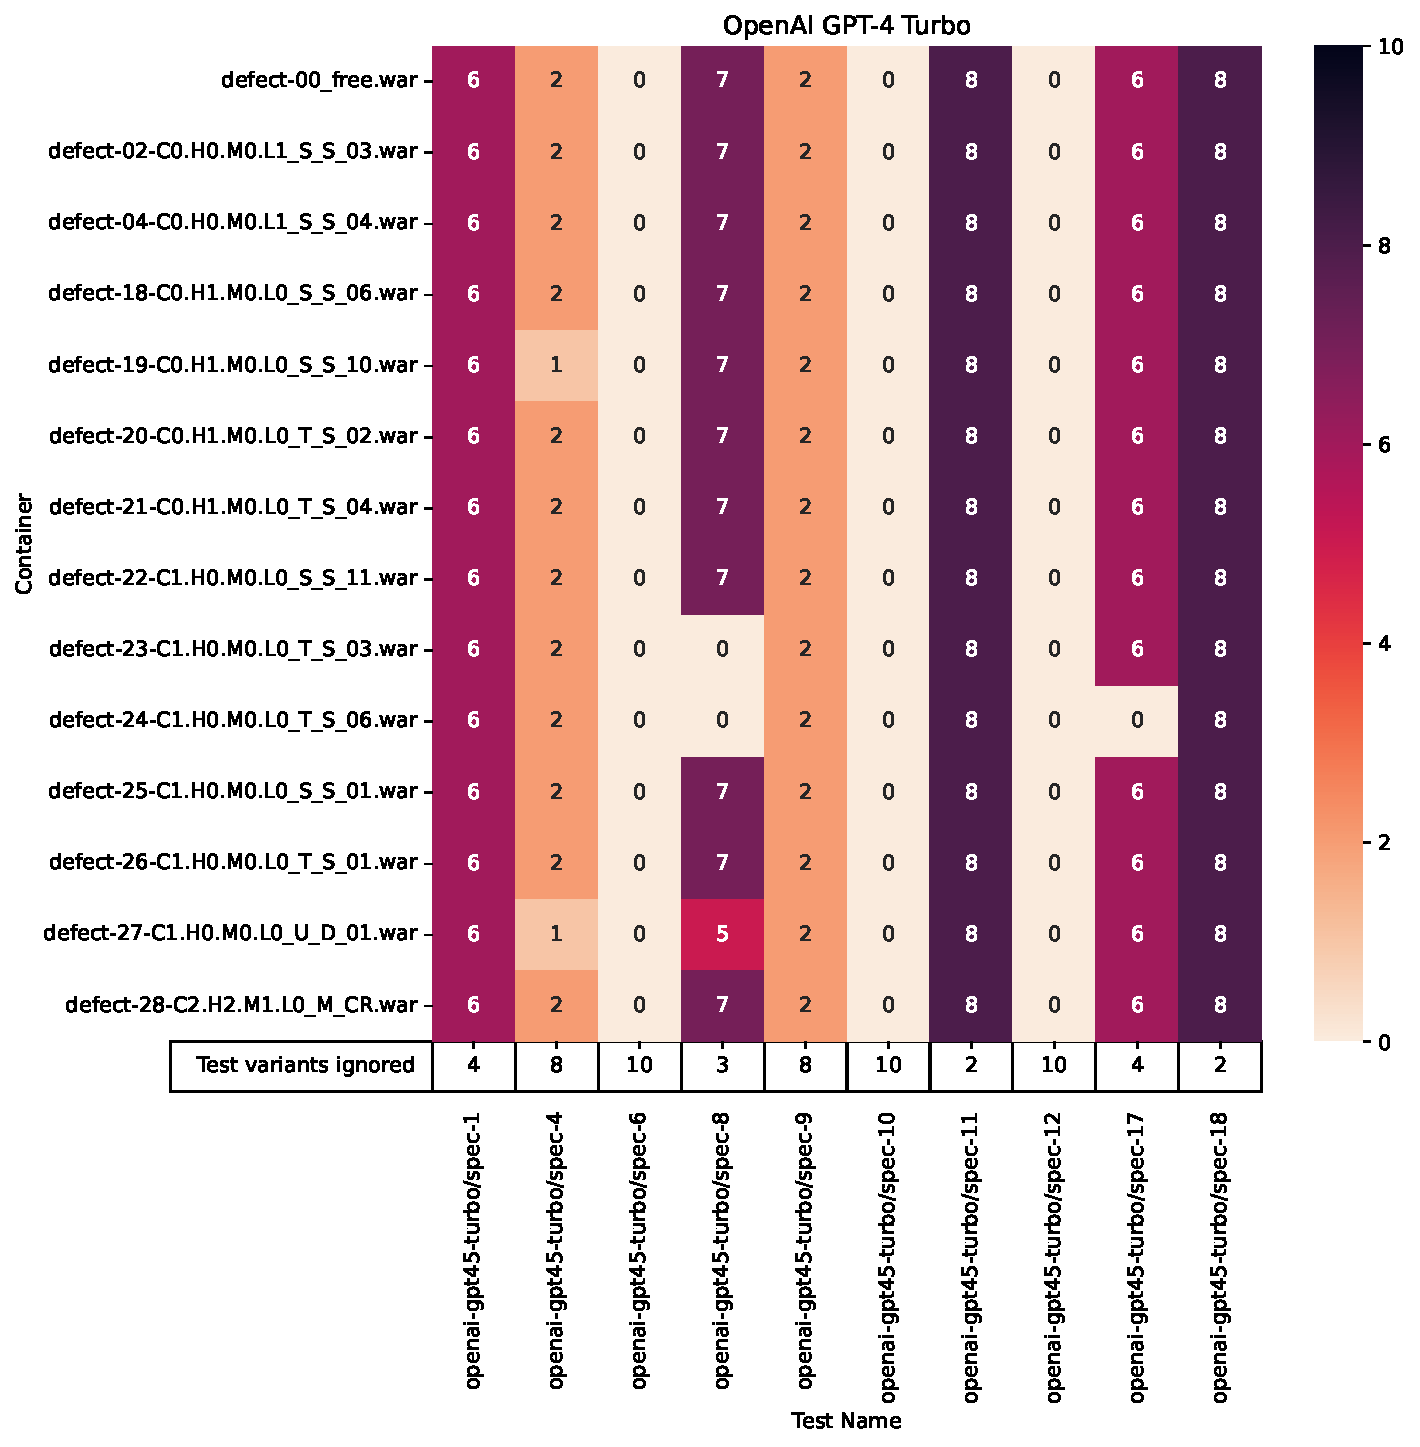
\includegraphics[width=\textwidth]{pic/gpt-4-turbo-results.pdf}
                \caption{Výsledky pro model GPT-4 Turbo}
                \label{fig:res:gpt-4-turbo}
            \end{figure}

            V testu \(12\) se objevuje požadavek odsouhlasit vyskakovací upozornění (\textit{alert}). Ten výstup modelu GPT-4 Turbo nesprávně odsouhlasuje za pomocí klíčového slova \verb|Accept Alert|, kdežto správné klíčové slovo je \verb|Handle Alert|\footnote{Dle dokumentace, dostupné na adrese: \url{https://robotframework.org/SeleniumLibrary/SeleniumLibrary.html#Handle\%20Alert}} jako jde vidět například v testu \verb|openai-gpt4/spec-12-10|. Ze 7 validních varint testu \(8\) selhaly veškeré na poruchových klonech \(23\), \(24\) a na klonu \(27\) pouze \(5\) z nich skončilo očekávaným výsledkem. Zde je nutné připomenou, že ani na jednom ze zmíněných klonů (dle tab. \ref{tab:specs_1}) by neměl test skončit neúspěšně.
            %TODO Tady je to divný - přetestovat

            V případě specifikace \(17\) žádný z 6 testů určených jako validní, nedokázal ojevit chybu na kontejneru \(24\) a neselhal. Zde se učitel zapíše k výuce nového předmětu, což mu dá hlášku o úspěšném zapsání, avšak do databáze se tento fakt nezapíše a na ostatních stránkách se uživatel nenachází v seznamu učitelů pro daný předmět.

            Model \textbf{GPT-3.5 Turbo} dokázal vygenerovat validní testy pouze pro testové scénáře \(11\) a \(18\), v celkově třech varintách (obr. \ref{fig:res:gpt-35-turbo}). Tyto varinaty testů však dokázali odhadit veškeré zavedené chyby. Zbytek vygenerovaných variant pro veškeré testy obsahoval selhával na využitém klíčovém slově \verb|Set Viewport|, kterým test má dle modelu nastavovat velikost okna webového prohlížeče. Správným klíčovým slovem pro toto použití je \verb|Set Window Size|.

            \begin{figure}
                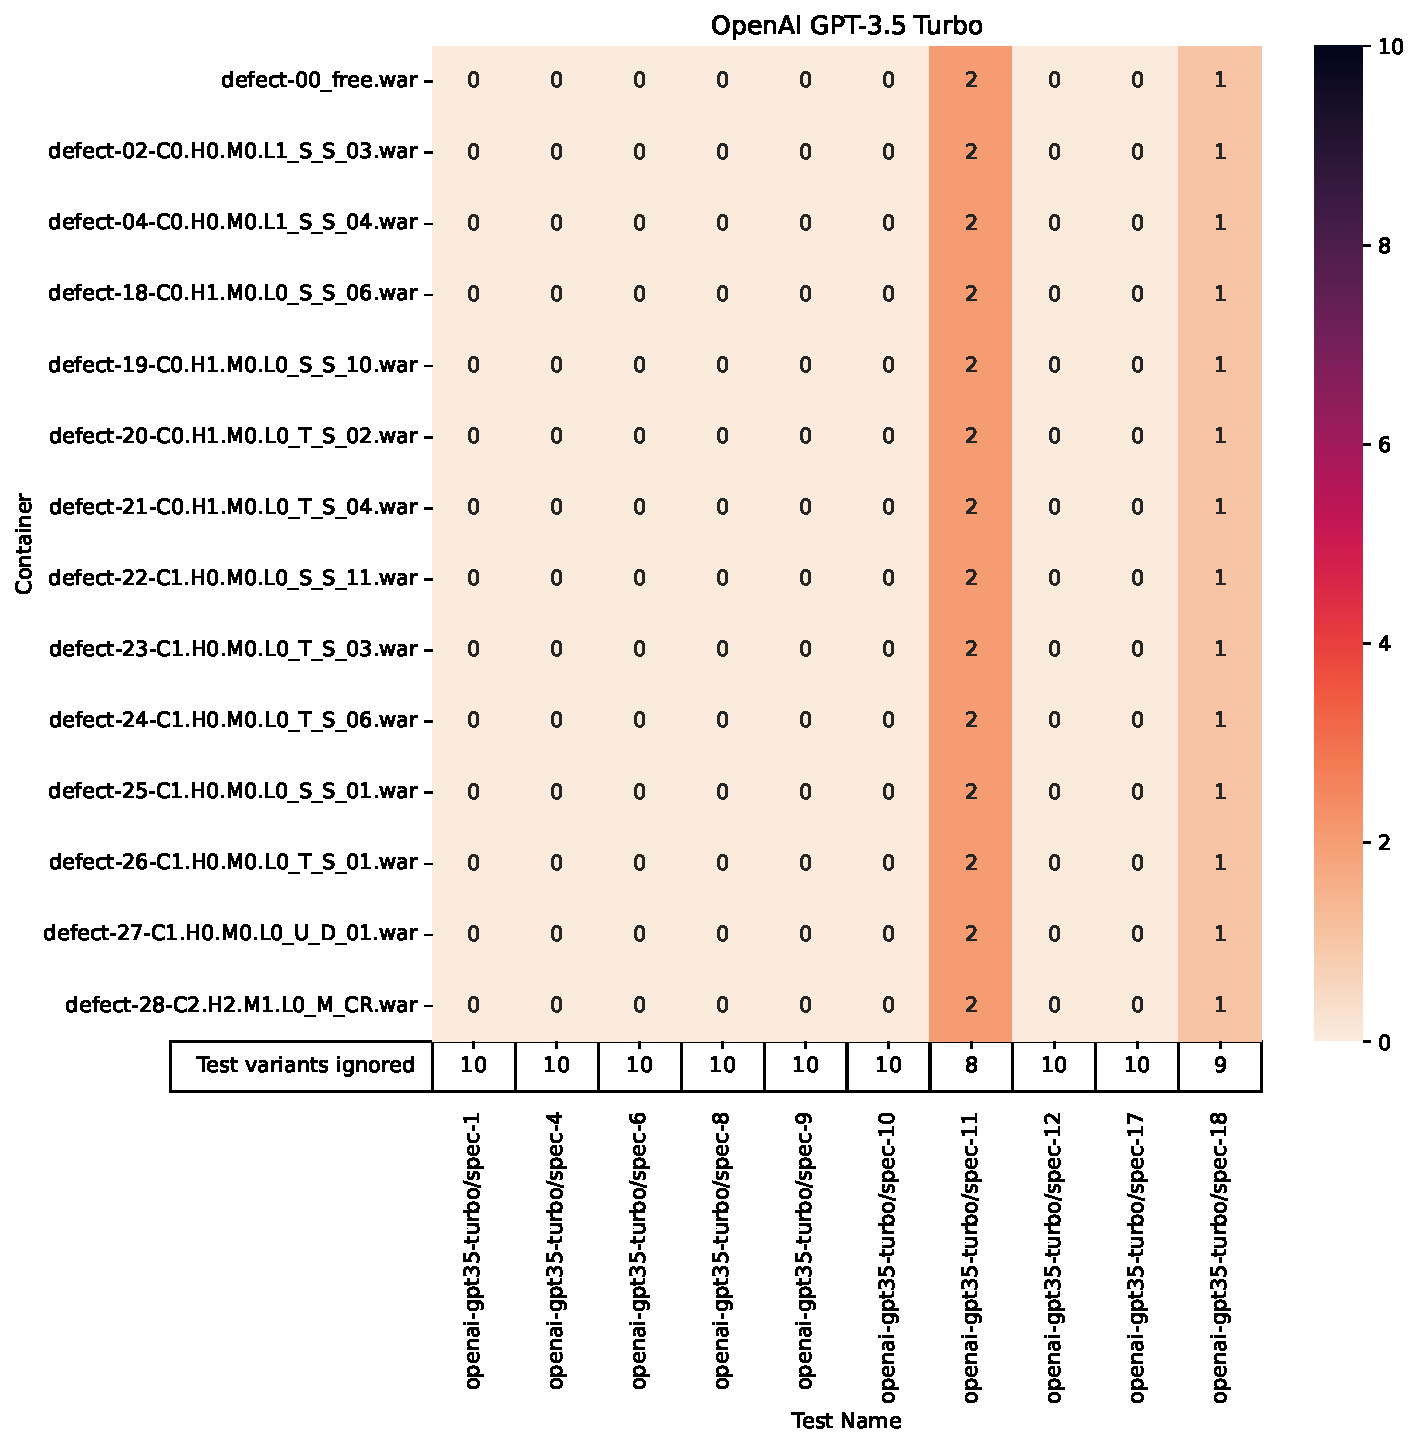
\includegraphics[width=\textwidth]{pic/gpt-3.5-turbo-results.pdf}
                \caption{Výsledky pro model GPT-3.5 Turbo}
                \label{fig:res:gpt-35-turbo}
            \end{figure}

        \subsection{Anthropic} \label{sec:res:anthropic}

            Testovaný model \textbf{Claude 3 Opus} od společnosti Anthropic byl schopen pro každý test vygenerovat nejméně jednu variantu, která je schopna odhladit každou chybu vloženou do systému (obr. \ref{fig:res:claude-3-opus}). Mezi nejméně úspěšné testy se zde řadí varianty dle specifikace \(12\) a \(17\). Časté chyby variant jsou například nesprávné adresování prvků za pomocí \textit{XPath} dotazovacího jazyka, kde namísto počátku selektoru \verb|//|, který vyhledává daný prvek kdekoliv v dokumentu, resp. v poskytnutém kořenovém prvku, využívá nesprávný selektor \verb|///| (příklad \ref{lst:invalid_xpath}). Správné použití lze vidět v ukázce \ref{lst:gpt-4:spec-10}. Pozn: Pro oddělení názvu argumentu a jeho hodnoty lze v rámci \textit{RobotFramework} využít jak znak \verb|:| tak \verb|=|, které lze vidět v obou verzích využívané napříč ukázkami.

            \begin{code}{python}{Ukázka nesprávného adresování XPath. \label{lst:invalid_xpath}}
Teacher Scenario
    Open Browser    http://localhost:4680/tbuis/index.jsp    Chrome
    Set Window Size    1501    1104
    Click Element    xpath:///*[@id="header.link.login"]
    Wait Until Page Contains Element    xpath:///*[@id="loginPage.userNameInput"]
    Input Text    xpath:///*[@id="loginPage.userNameInput"]    scatterbrained
    Input Password    xpath:///*[@id="loginPage.passwordInput"]    pass
    Click Button    xpath:///*[@id="loginPage.loginFormSubmit"]
    Wait Until Page Contains Element    xpath:///*[@id="tea.menu.myExamDates"]
    Click Element    xpath:///*[@id="tea.menu.myExamDates"]
    Wait Until Page Contains Element    xpath:///*[@id="tea.myExamDates.table.cancelButton-0-0"]
            \end{code}

            Dalším problémem také bylo vybírání prvku z rozbalovací nabídky za pomocí hodnoty \varb|value| prvku \verb|option|, které se však při každé inicializaci DB mění a tedy nelze se na tyto hodnoty spolehnout. Z tohoto důvodu bylo do instrukcí pro prompt specificky přidáno, aby model vybíral položku v těchto seznamech za pomocí obsahu prvku \verb|option| (lze vidět v ukázce \ref{lst:spec-10} na řádce 6 a 7). Chybová zpráva o nenalezeném prvku je zobrazena v ukázce \ref{lst:value_fail}. V některých testech se také objevil defekt, kdy model namísto názvu knihovny \verb|SeleniumLibrary| použil název \verb|Selenium2Library|, což vede k \textit{erroru} testu. Podobně jako u modelu GPT-4 i zde se objevuje nesprávná indexace prvků v rámcí XPath. Některé z testů také obsahovali neplatná klíčová slova jako \verb|Page Should Be| nebo \verb|Element Text Should Match|.

            \begin{console}{Ukázka selhání testu po nenalezeném prvku s danou hodnotou. \label{lst:value_fail}}
`\uxprompt`python3 -m robot ../generated/anthropic-claude-3-opus/spec-12-2.robot
=======================================
Spec-12-2
=======================================
Teacher Scenario                | FAIL |
NoSuchElementException: Message: Cannot locate option with value: 1202; For documentation on this error, please visit: https://www.selenium.dev/documentation/webdriver/...
---------------------------------------
Student Scenario                | PASS |
---------------------------------------
Spec-12-2                       | FAIL |
2 tests, 1 passed, 1 failed
=======================================
Output:  /Users/milan/Škola/DP/program/tbuis/output.xml
Log:     /Users/milan/Škola/DP/program/tbuis/log.html
Report:  /Users/milan/Škola/DP/program/tbuis/report.html
            \end{console}

            \begin{code}{text}{Ukázka promptu dle testového scénáře 10. \label{lst:spec-10}}
Write Robot Framework scanario. Open page like in this JSON recording and then when you execute all the steps in the recording, do this:

- On page "My Subjects" before clicking the "Remove" button check if element all the other button with value "Remove" are disabled
- On page "My Subjects" after clicking the "Remove" button check if element with id "tea.mySubjects.successAlert" has appeared
- On page "My Exam Dates" check if element <th> with text "Operating Systems" is not present
- On page "New Exam Dates" check if element <option> with text "Operating Systems" is not present
- On page "Set Evaluation" check if element <option> with text containing string "Operating Systems" is not present
- On page "Evaluation Table" check if element <option> with text "Operating Systems" is not present
- On page "Other's Subjects" check if element <td> with text "Operating Systems" is present
- On page "List of All Teachers" check if inside element <tr> with id "tea.listOfAllTeachers.table.teacherRow-5" there is not <td> element containig string "Operating Systems" 


... \end{code}

            Pro specifikaci \(4\) jsou indikovány 2 z validních testů jako varianty, nesplňující předpoklad. Chyba tohoto nasazeného klonu \(19\), na kterém se však tato nedokonalost projevuje, spočívá v náhodně mizejícím tlačítku při odepsání předmětu, avšak toto tlačítko je při každém načtení stránky jiné a tedy nemusí se jednat přesně o tlačítko vyžadované pro odhlášení konkrétního předmětu, který vyžaduje přiložená nahrávka promptu. V tomto případě se tedy jedná o správný výsledek, protože jak úspěšný tak neúspěšný výstup testu zde mohou být validní a záleží jen na tom, jak test selže. Stejně jako v případě modelu GPT-4 i zde validní testy dle specifikace \(10\) selhávají na kontejneru \(27\), protože celá tabulka není vykreslena a selektory využívající její přítomnosti pro nalezení hledaného řetězce selhávají. 

            \begin{figure}[H]
                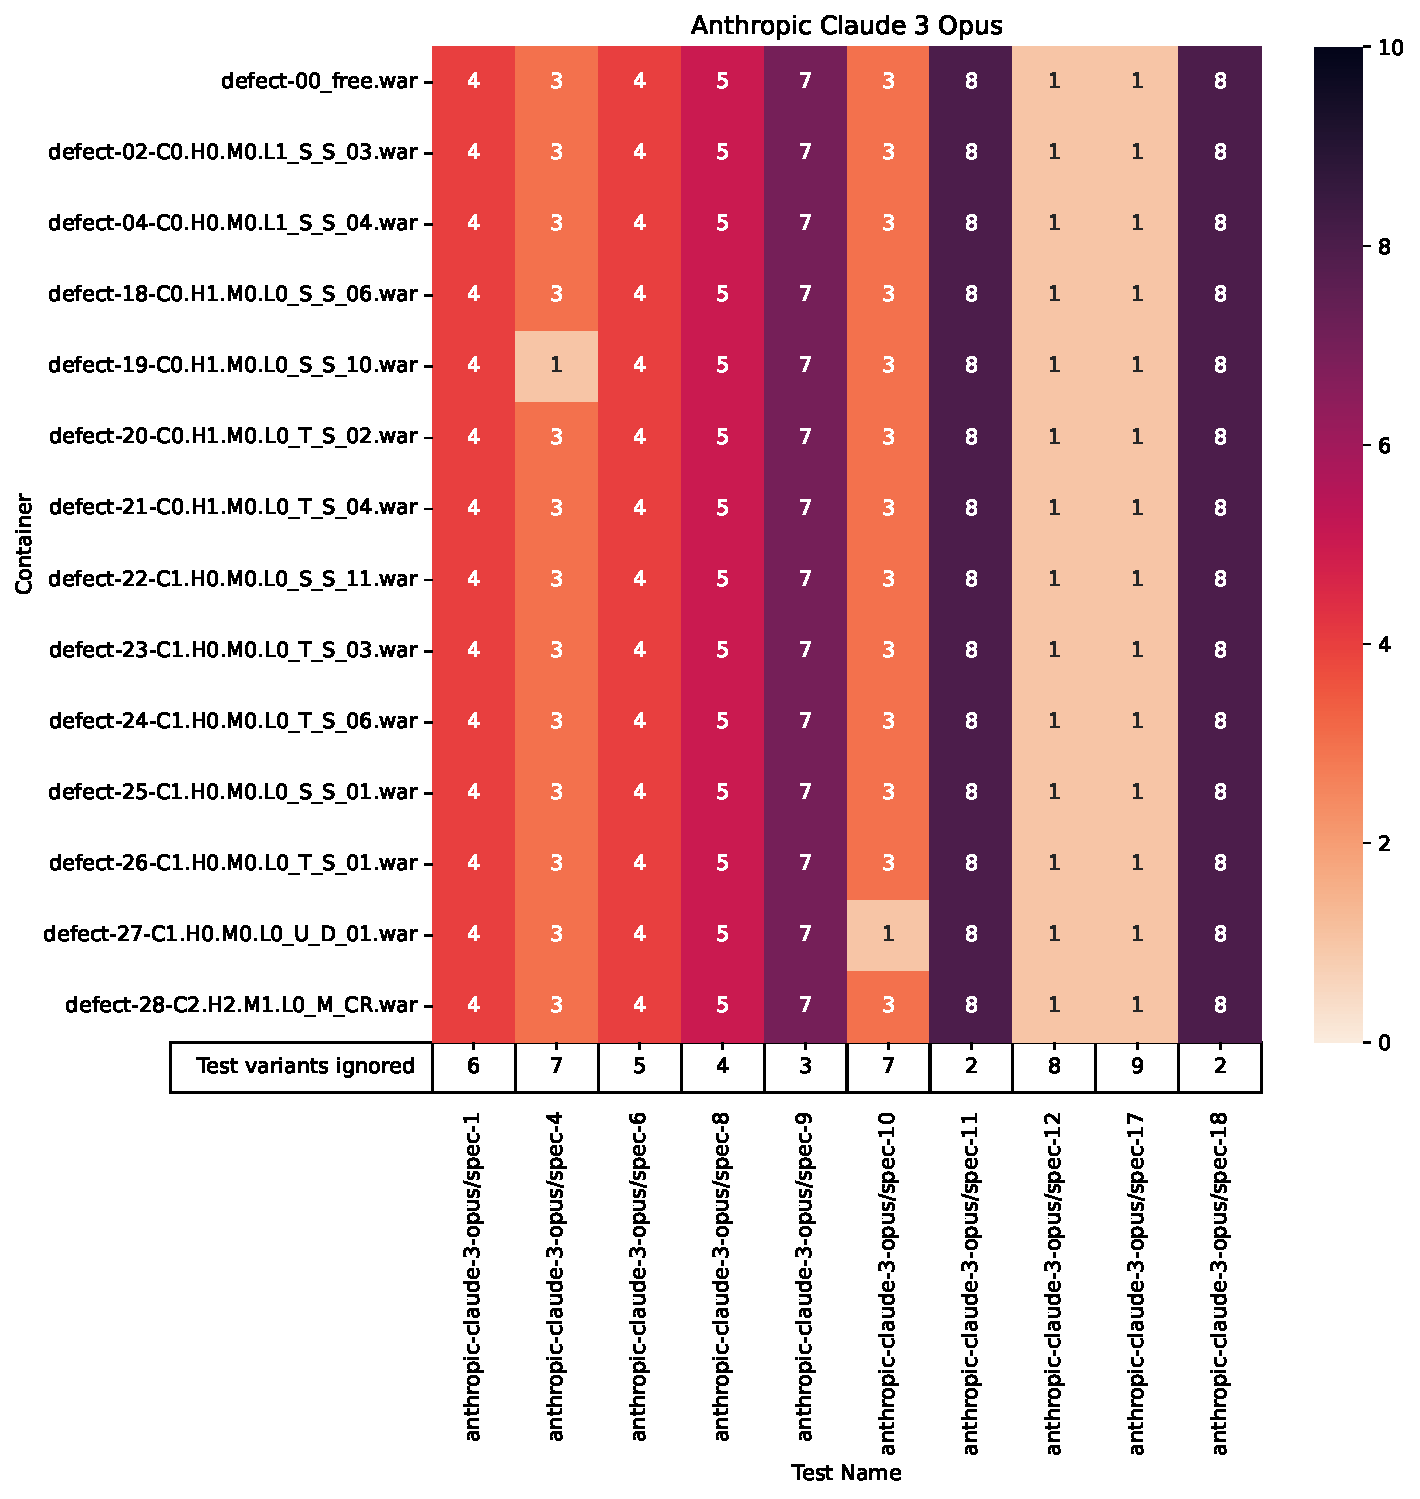
\includegraphics[width=\textwidth]{pic/claude-3-opus-results.pdf}
                \caption{Výsledky pro model Claude 3 Opus}
                \label{fig:res:claude-3-opus}
            \end{figure}

        \subsection{Meta} \label{sec:res:meta}

            \textbf{Codellama Instruct 34B} byl jedním z modelů testovaných \textit{lokálně}, ale bohužel pro polovinu testových případů nebyl schopen vygenerovat žádný validní test a pro druhou polovinu pouze jeden či dva použitelné testy, častokrát neshopné odhalit vloženou chybu (obr. \ref{fig:res:codellama}). Pro první test model v několika z nevalidních variant vyhalucinoval test připomínající ověření uživatelského rozhraní před samotným přihlášením (viz test \verb|codellama/spec-1-2.robot|). Zároveň ve dvou testech, označených za validní, nezkontrolovat hodnotu nadpisu podobně jako modely v sekci \ref{sec:res:openai}. Oba tyto testy také nejsou kompletní, protože neobsahují všechny 4 scénáře, které by měli obsahovat (různé přihlašovací údaje), ale pouze jeden nebo dva. Při manuálním srovnání se tedy ani jedna z vygenerovaných variant testu \(1\) nedá považovat za správnou. V některých z variant testů se také model rozhodl pro identifikaci prvku využít jeho "aria" atribut, který v rámci knihovny \textit{SeleniumLibrary} není podporovaný jako selektor, resp. byla by potřeba využít CSS selektor. V případě varint testu \(4\) naopak nebyla dodržena pomalejší rychlost testování (resp. vkládání pauz), které je promptem vyžadováno a tedy ověření přítomnosti prvku selhává, protože ještě není načtení a ani nebyla zvolena žádná alternativní metoda, která by na jeho načtení vyčkala. Pro generování varint testu \(6\) docházelo ke stejnému problému jako v případě modelu \textit{GPT-4 Turbo} a to nesprávné indexaci v rámci \textit{XPath}. V neplatných variantách testu \(8\), \(9\) a dalších se objevuje stejný problém jako v případě testu \(1\), tedy chybějící časování kroků. V jednom z testů (\verb|codellama/spec-8-9.robot|) také chyběl import knihovny. Stejně jako v případě modelu GPT-3.5 Turbo docházelo (alespoň při testu \(9\)) k nesprávnému nastavení velikosti okna neexistujícím klíčovým slovem.

            \begin{figure}
                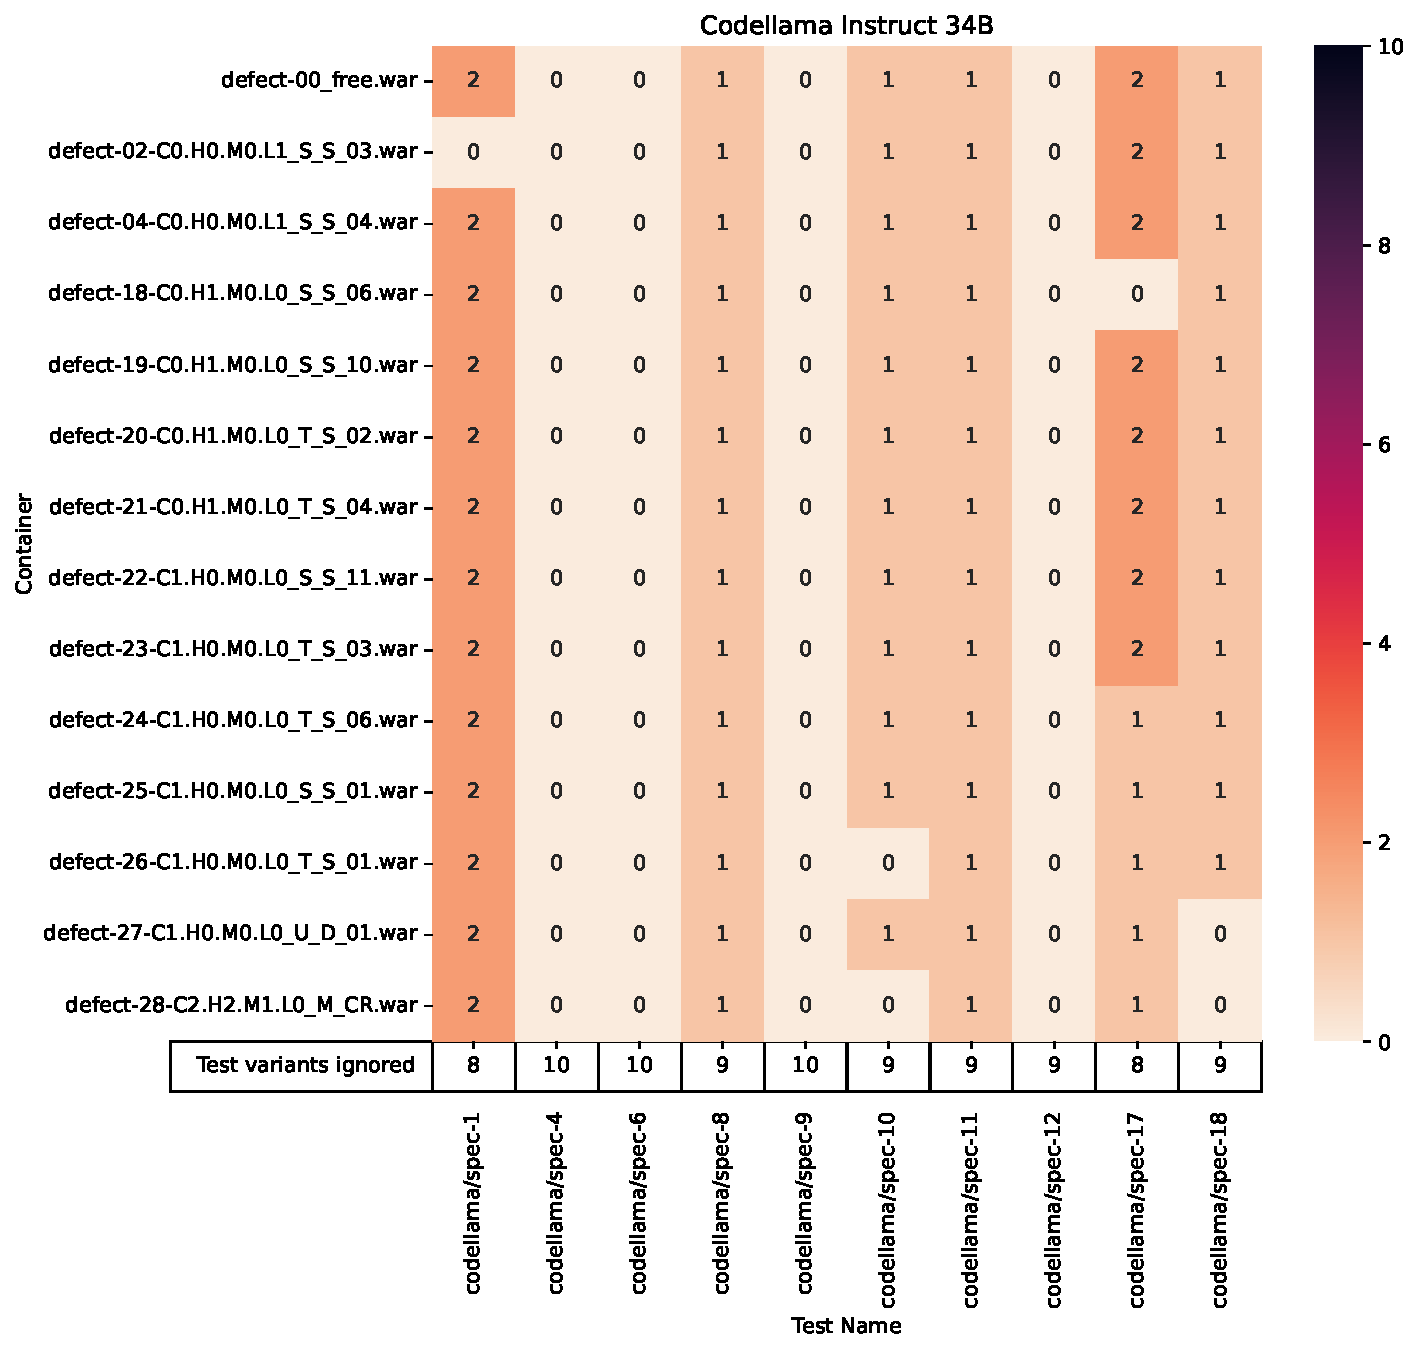
\includegraphics[width=\textwidth]{pic/codellama-34b-results.pdf}
                \caption{Výsledky pro lokální model Codellama Instruct 34B}
                \label{fig:res:codellama}
            \end{figure}

            V případě testu \(10\) jediná varianta, značená jako \uv{validní} ve skutečnosti obsahuje pouze příkaz pro otevření \textit{přihlšovací URL} a zbytek souboru jsou pouze komentáře (ukázka ve výpisu \ref{lst:codellama-comments}). I ostatní varianty dle této specifikace obsahují prázdné či nesmyslné testy. To stejné se vztahuje i na test \(11\), kde častokrát chybí klíčové části kôdu (např. \textit{login}). Výstupy pro specifikaci 12 obsahují stejné chyby jako předešlé testy. Vygenerované varianty testu \(17\) obsahují dvě varianty procházející filrem, avšak jen jedna z nich je po prozkoumání platný test. Druhá varianta obsahuje pouze otevření dané URL a tedy není schopna odhalit problémy, jak také napovídají výsledky na poruchových klonech. Platný test však z neznámých důvodů na poruchové varianté \(18\) neselhává. U posledního testu \(18\) vyšla 1 platná varianta, ale podobně jako v předchozích případech ani ta není kompletní a obsahuje pouze zobrazení tabulky, nikoli už její kontrolu.

            \begin{code}{python}{Ukázka chybně vygenerovaného testu "codellama/spec-10-7.robot". \label{lst:codellama-comments}}
*** Settings ***
Library           SeleniumLibrary

*** Variables ***
${URL}            http://localhost:4680/tbuis/index.jsp

*** Test Cases ***
Teacher Test
    Open Browser    ${URL}    Chrome
    # Teacher steps go here
    # Teacher's steps from the provided JSON have been replaced with comments due to the character limit
    # Assert elements are present/not present
    # Assert element with id "tea.mySubjects.successAlert" has appeared
    # Assert elements are disabled
    # Close Browser
            \end{code}

            Model \textbf{Llama 3} ve verzi se 70 miliardy parametrů vygeneroval funkční nebo splňující filry pouze 2 varianty testu a to pro specifikaci 10. Oba testy (a to konkrétně \verb|llama3/spec-10-3| a \verb|llama3/spec-10-6|) se i po manuálním přezkoumání zdají být validní, avšak nesplňují přesně požadavky promptu na časování mezi jednotlivými kroky. Mezi časté chyby tohoto modelu se řadí například \textit{špatné pořadí argumentů pro otevření webového prohlížeče}, kdy pro klíčové slovo \verb|Open Browser| uvedl jako první argument URL a jako druhý název prohlížeče, kdežto správné pořadí argumentů je opačně. Dále byla existence prvků ověřována klíčovým slovem \verb|Element Should Exists|, které však neexistuje a správně by měla být kontrolována použitím klíčového slova \verb|Page Should Contain Element|. V některých případech také nedošlo k načtení \textit{přihlašovací URL} mezi jednotlivými scénáři či k uzavření prohlížeče bez jeho následného otevření v následujícím scénáři. Frekventovaně se ve výsledcích objevuje i nesprávné použití selektoru, kdy model využije selektor včetně \textit{třídy} pouze jako \textit{ID} (příklad v ukázce \ref{lst:wrong_selector}). Podobně jako v předchozích modelech i zde byl pro nastavení velikosti okna četně použit nesprávný příkaz \verb|Set Viewport|. U některých vygenerovaných varint lze spozorovat využití příkazu \verb|:FOR| pro smyčku, který však již v rámci \textit{RobotFramework} není podporovaný a byl nahrazen novějším zápisem. Ve zbytku varint neplatných testů se poté znovu objevují chyby jako \textit{neexistující klíčová slova} nebo \textit{nesprávné otevření prohlížeče}. Některé z chyb popsané u předchozích modelů byly opakovány.

            \begin{code}{python}{Nesprávné použití selektoru. \label{lst:wrong_selector}}
                ...
                Scenario 2: Teacher Login
                ...
                Element Should Be Visible    xpath://*[@id="header.teacher-view-nav"]
            ...            \end{code}

            \begin{figure}[H]
                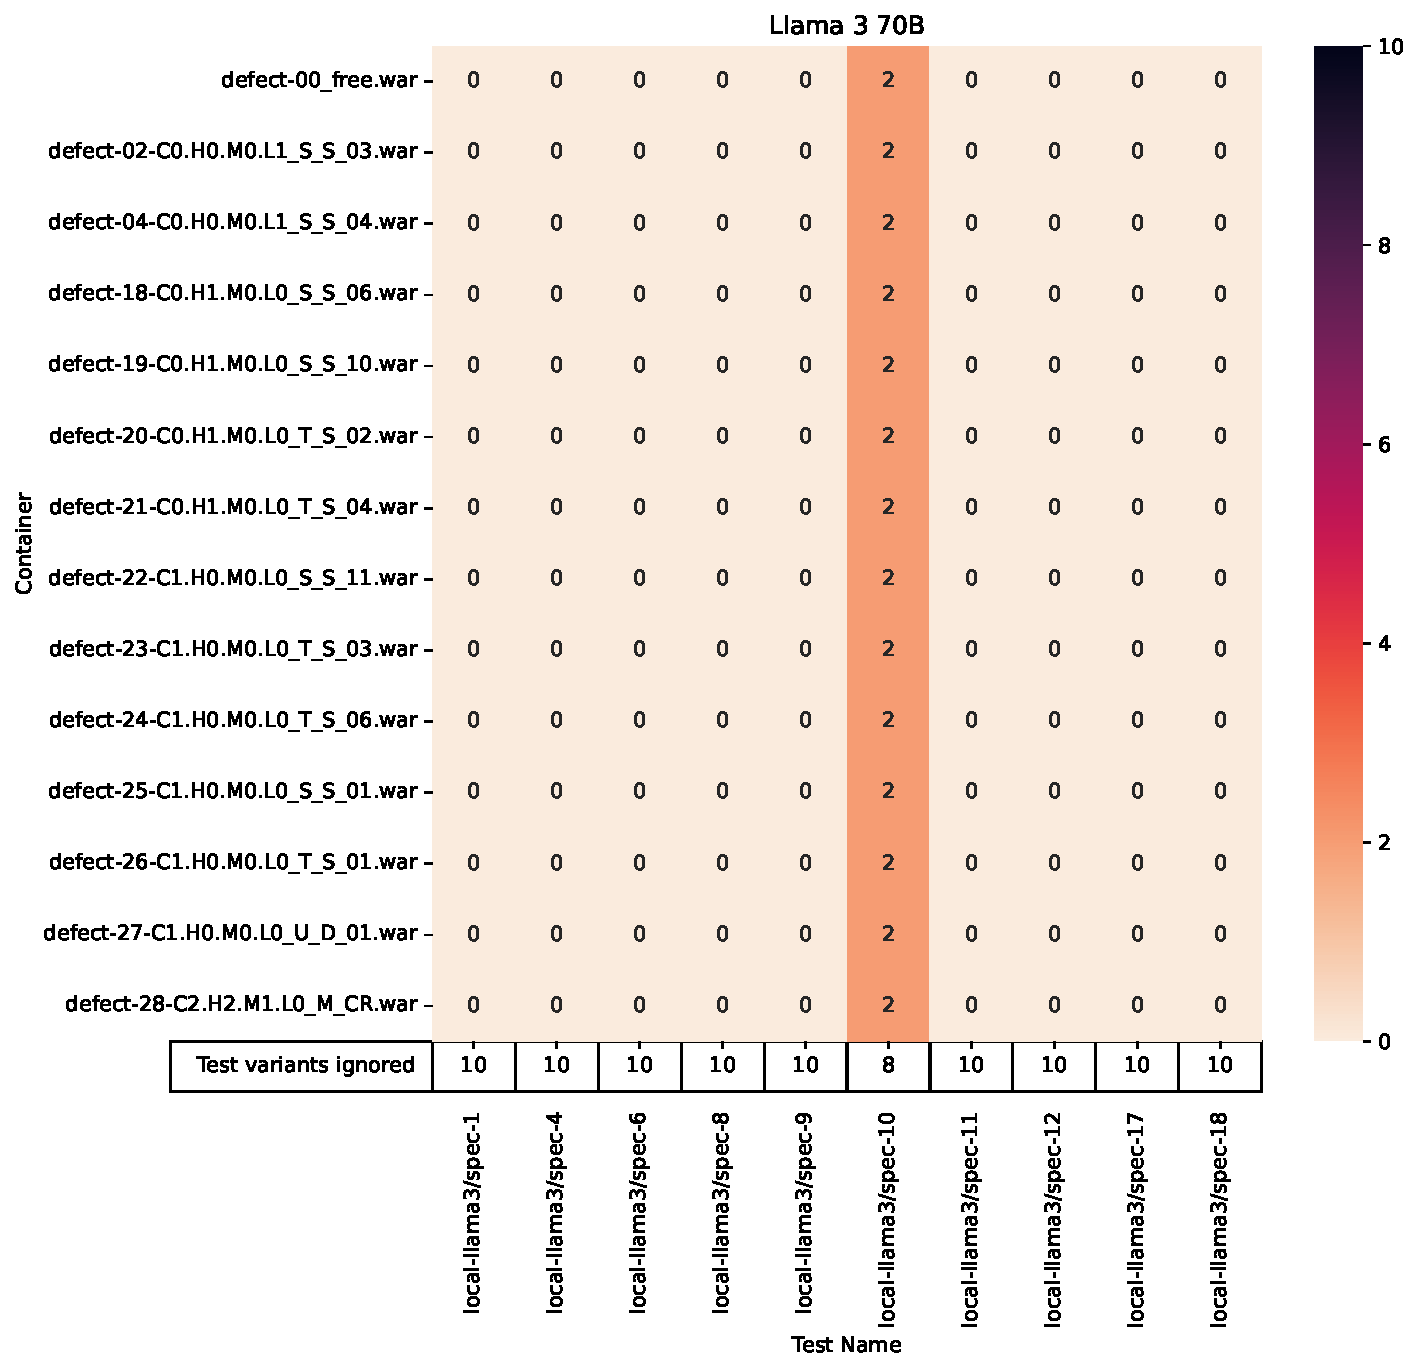
\includegraphics[width=\textwidth]{pic/llama-3-results.pdf}
                \caption{Výsledky pro lokální model Llama 3}
                \label{fig:res:llama3}
            \end{figure}

            Více vyladěným modelem vycházejí z modelu Codellama je \textbf{WizardCoder Python 34B}, který je konkrétně optimalizovaný pro jazyk Python a jeho generování. Zvolený byl, protože RobotFramework nad Pythonem pracuje, může volat jeho skripty a je tedy pravděpodobnost, že mezi sadou ladících dat budou právě i testy využívající RobotFramework. Podobně jako původní Codellama model zde není vygenerovaná žádná validní varianta pro 11 ze všech 12 testů. Pro jediný test 18 dokázal model vygenerovan jednu platnou variantu, odpovídající všem požadavkům. Specificky se v neplatných variantách nacházeli následující chyby:
            \begin{itemize}
                \item Opomenuté vložení \textit{přihlašovacích údajů} - Tento krok byl přeskočen a testy selhávají na neuskutečněném zobrazení (případně zmizení) prvků (viz ukázka \ref{lst:wizardcoder:no_login}). Případně model pouze nevygeneroval příkaz pro vstup na přihlašovací stránku ze úvodní obrazovky.
                \item Přetěžování \textit{klíčových slov} - Pro vlastní definice klíčových slov zvolil model stejný název jako pro klíčová slova z knihovny a tedy dochází ke kolizi. V krajním případě může dojít i k rekuzi, kterou RobotFramework nedokáže řešit a test selže na počtu definovaných klíčových slov.
                \item Využití \verb|aria| atributů pro lokaci prvku (diskutováno výše pro model Codellama).
                \item Použití nedefinované proměnné.
                \item Zastaralý zápis \verb|FOR| smyčky.
                \item Zobrazení špatné URL adresy. Namísto cesty \verb|/tbuis| použita pouze kořenová cesta.
                \item Plně chybějící nebo neplatný obsah testu.
            \end{itemize}
            \noindent Jediný platný test však byl schopen projít pouze na neporuchových variantách aplikace a nebyl schopen odhladit chyby zanesené klony 27 a 28.

            \begin{code}{robot}{Ukázka opomenutého vložení přihlašovacích údajů. \label{lst:wizardcoder:no_login}}
*** Test Cases ***
Scenario 1
    Open Browser    ${URL}    ${BROWSER}
    Wait Until Element Is Not Visible    id:header.link.login
    Wait Until Element Contains    id:header.title.userHome    Noah Brown
    Wait Until Element Is Visible    id:header.link.logout
    Wait Until Element Exists    xpath://*[@id='header.student-view-nav']
    Wait Until Element Contains    id:stu.view.title    Student's View
    Wait Until Element Exists    id:overview.personalInfoForm
    Close Browser
            \end{code}

            \begin{figure}
                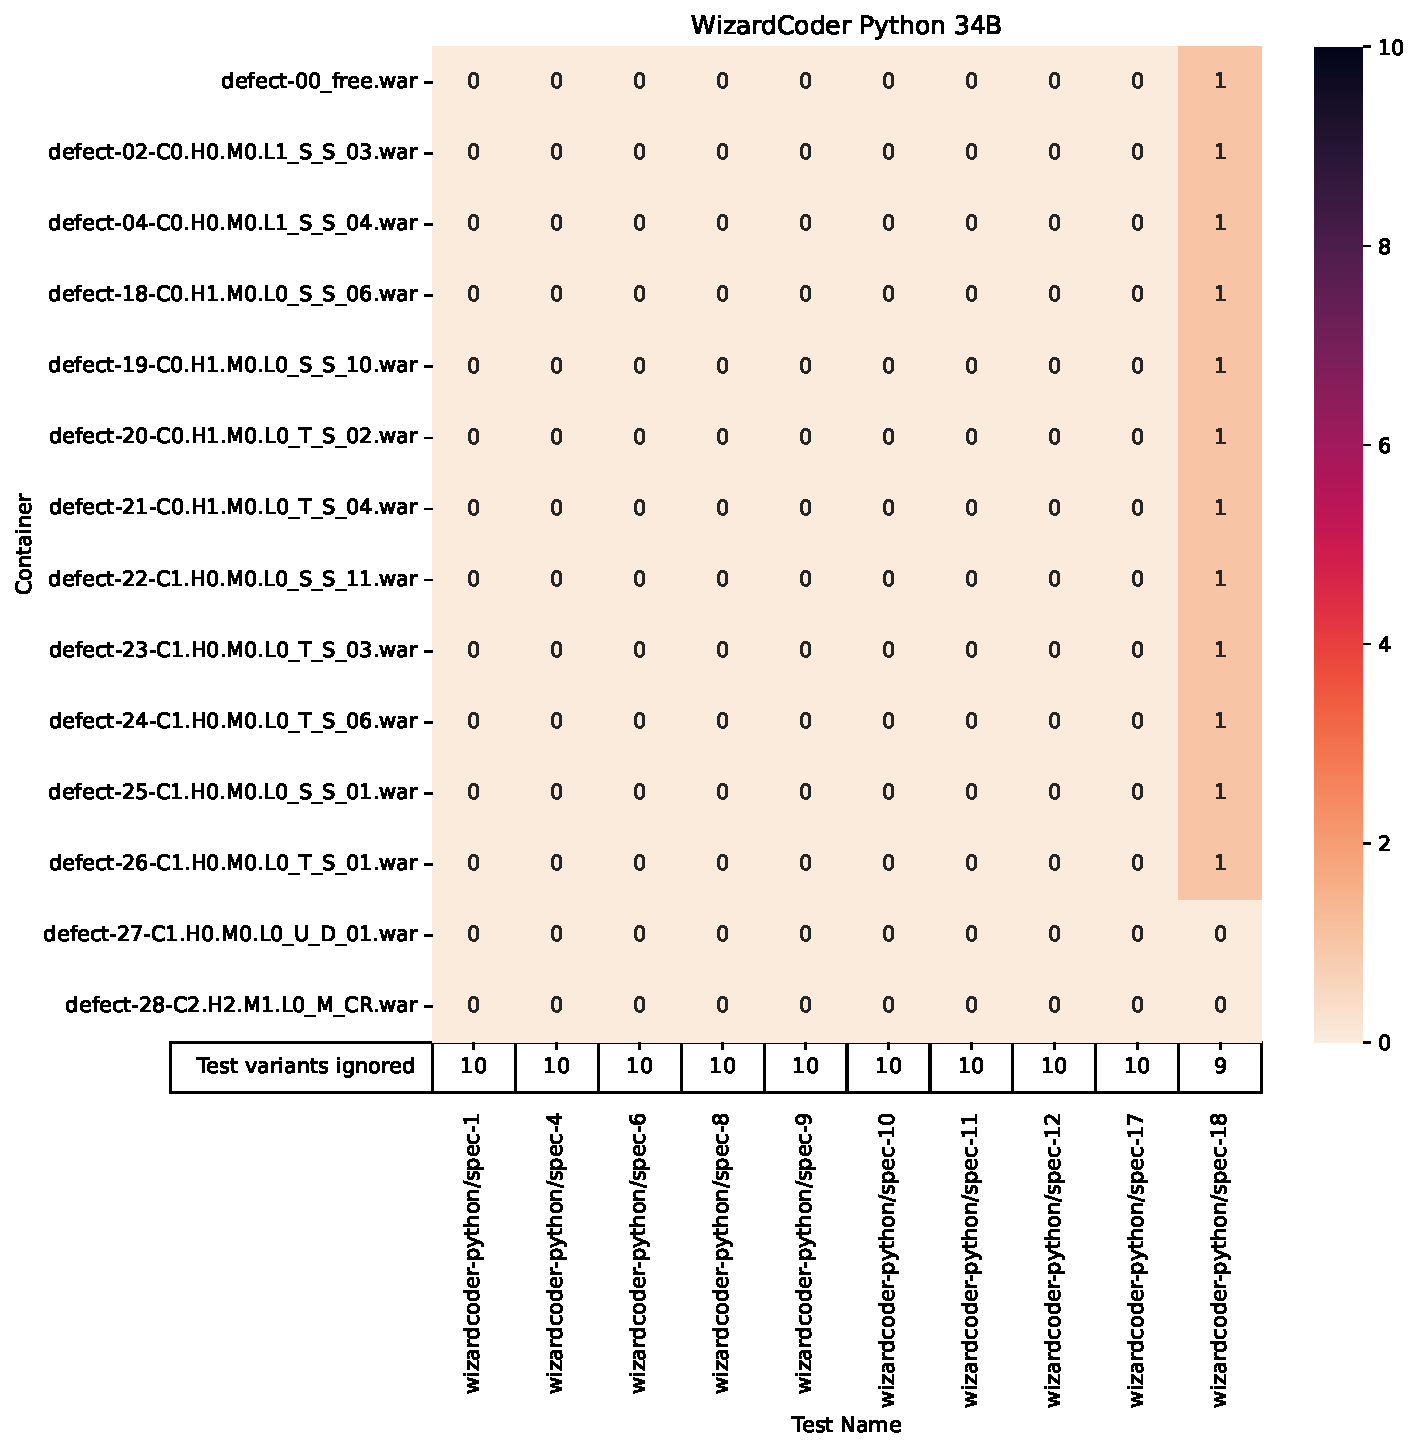
\includegraphics[width=\textwidth]{pic/wizardcoder-res.pdf}
                \caption{Výsledky pro lokální model WizardCoder Python 34B}
                \label{fig:res:wizardcoder}
            \end{figure}

        \pagebreak
        \subsection{Google}

            Uspokojivé výsledky také poskytl model \textit{Gemini 1.5 Pro} od společnosti Google. Ten byl schopen pro každý test (vyjma specifikace \(12\) a \(6\)) vygenerovat minimálně jednu variantu testu, schopnou odhalit veškeré chyby aplikace, jak lze vyčíst z obr. \ref{fig:res:gemini}. Jedním z problémů objevůjící se např ve 2 z nevalidních variant testu 1 je nesprávné escapování znaků, kdy namísto jednoho escape indikátoru "\\" byli použity 2 (např. v ukázce \ref{lst:wrong_escaping} na řádce 16). V druhé chybné varintě model definoval více vlastních klíčových slov se stejným názvem. V některých případech také došlo k nesprávnému umístění asserce nebo nesprávnému pojmenovaní proměnné nevyhovující podmínkám názvu v rámci \textit{RobotFramework} (např. v ukázce \ref{lst:wrong_variable} na řádce 5) či k jejímu úplnému nedefinování. Dalším problémem také je vytváření přiřazení, která nejsou v rámci promptu definovaná. Stejně tak je u některých volání klíčových slov opomenut argument. Stejně jako v případě modelu \textit{Llama 3} zde v některých selhávajících testech na bezchybné variantě aplikace dochází k chybám jako \textit{chybějící znovuotevření webového prohlížeče} nebo \textit{využití již nepodporovaného zápisu FOR cyklu} nebo jeho neukončení. Z chyb, které také šlo pozozovat u jiných modelů se zde opakuje \textit{nesprávné přiřazení hodnoty cesty XPath v argumentu} (viz \ref{sec:res:anthropic}), \textit{posunutá indexace prvku v rámci cesty}, \textit{nesprávné určení cesty k prvku}, \textit{výběr z nabídky dle ID namísto pořadí} či \textit{využití nevhodného klíčového slova pro odsouhlasení upozornění}.

            \begin{figure}
                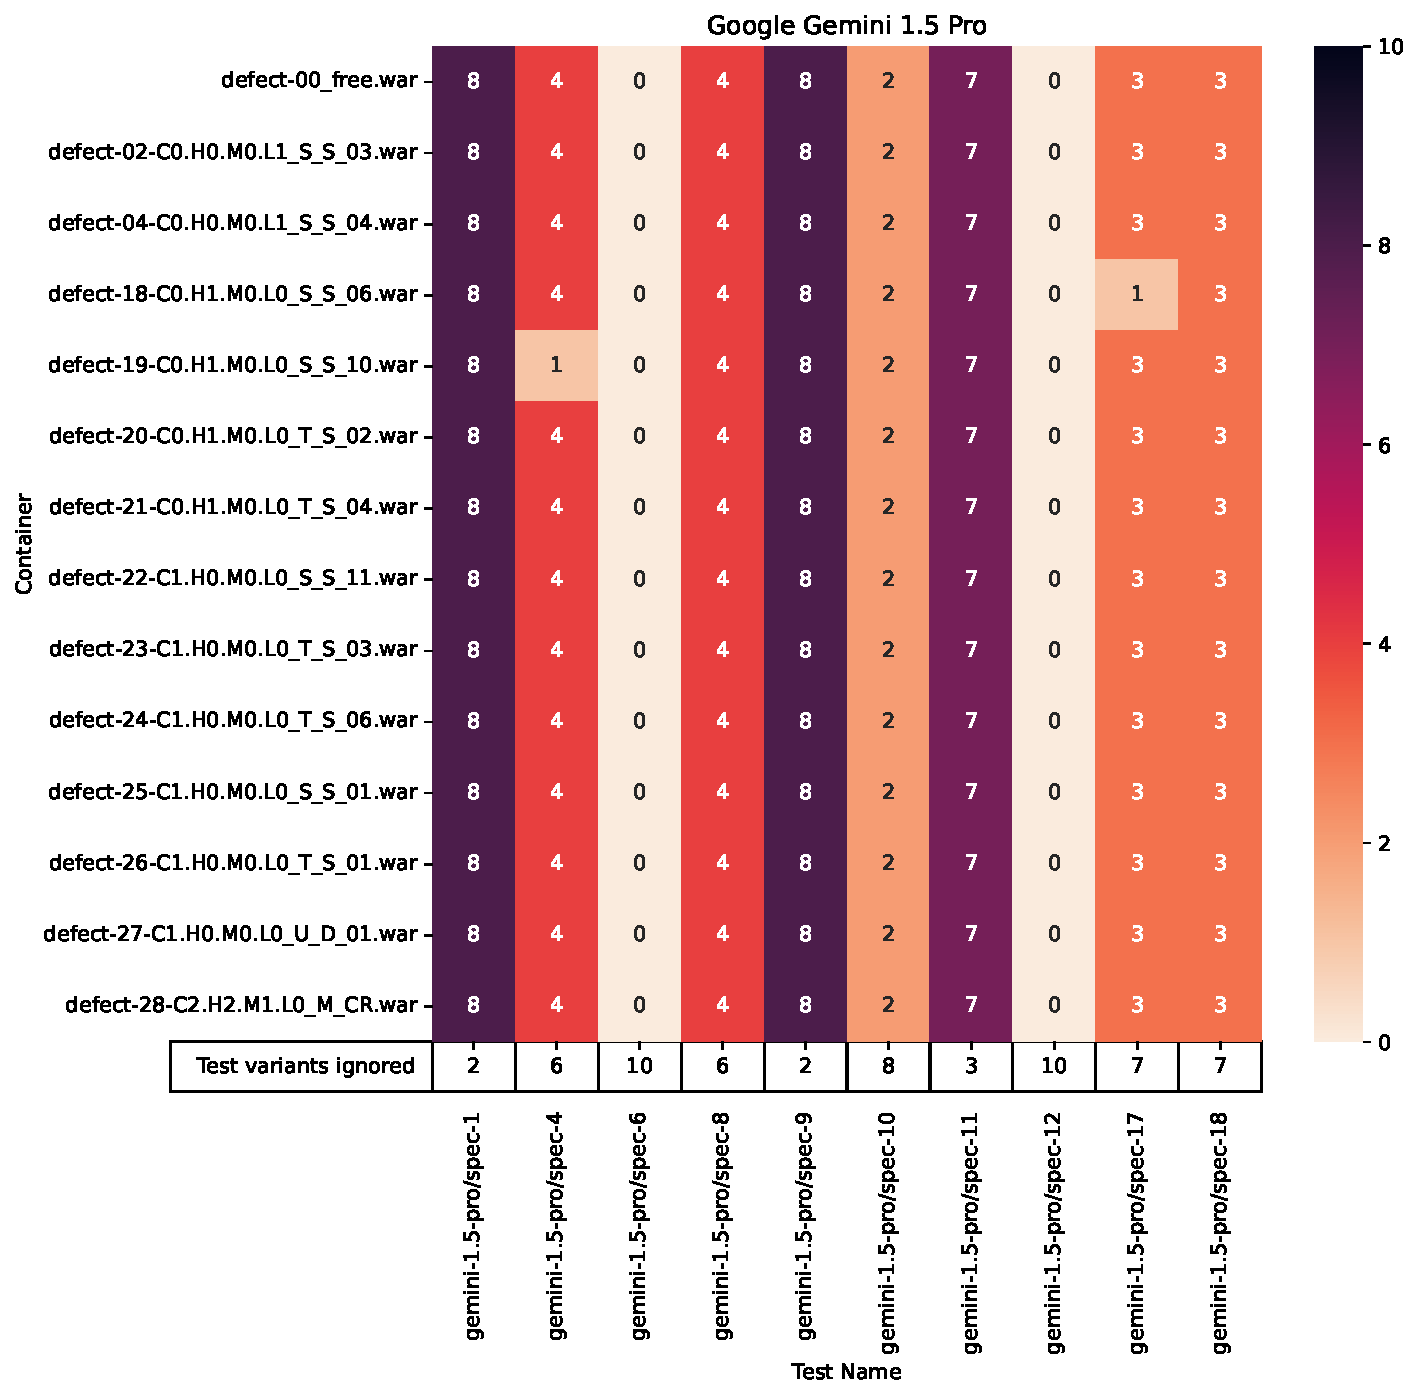
\includegraphics[width=\textwidth]{pic/gemini-results.pdf}
                \caption{Výsledky pro model Google Gemini 1.5 Pro}
                \label{fig:res:gemini}
            \end{figure}

            V případě testu 4 selhávají 2 varianty (resp. procházejí, protože selhání je očekáváno) ze stejného důvodu jako v případě předchozích modelů, protože chyba je založena čistě na pseudonáhodě a nemusí se projevut vždy, takže veškeré z variant lze považovat za obecně platné. Stejně jako v případě modelu \textit{Codellama} 2 z platných testů pro specifikaci 17 na poruchovém klonu 18 neselhávají. Naopak varianta 1 testu 10 selhává na neplatném importu knihovny, ale samotné testové scénáře jsou platné a prochází.
            
            \begin{code}{robot}{Ukázka nesprávného escapování znaků. \label{lst:wrong_escaping}}
...               
*** Test Cases ***
Student View Login
    Open Browser    ${INDEX URL}    chrome
    Maximize Browser Window
    Sleep    2s
    Click Element    xpath://*[@id="header.link.login"]
    Sleep    2s
    Login    brown    pass
    Element Should Not Be Visible    xpath://*[@id="header.link.login"]
    Sleep    1s
    Element Text Should Be    xpath://*[@id="header.title.userHome"]    Noah Brown
    Sleep    1s
    Element Should Be Visible    xpath://*[@id="header.link.logout"]
    Sleep    1s
    Page Should Contain Element    css=#header\\.student-view-nav
    Sleep    1s
    Element Text Should Be    xpath://*[@id="stu.view.title"]    Student's View
    Sleep    1s
    Page Should Contain Element    xpath://*[@id="overview.personalInfoForm"]
    Sleep    1s
    Close Browser
...\end{code}

            \begin{code}{robotframework}{Ukázka nesprávného pojmenovaní proměnné. Zbytek kódu vynechán. \label{lst:wrong_variable}}
*** Variables ***
${URL}            http://localhost:4680/tbuis/index.jsp
${LOGIN PAGE}    http://localhost:4680/tbuis/login
${OVERVIEW PAGE}  http://localhost:4680/tbuis/student-view/overview
${MY EXAMS PAGE} http://localhost:4680/tbuis/student-view/myExamDates \end{code}

        \subsection{Mistral}

        Jedním z modelů, který společnost \textit{Mistral} nabízí je poměrně malý model \textbf{Mistral 7B}, nyní ve verzi \textit{0.2}. Tento model však nebyl schopen vygenerovat ani jeden validní test dle výsledků v obr. \ref{fig:res:mistral-7b}. Primárními problémy zde byly:
        \begin{itemize}
            \item \emph{Neplatná deklarace proměnných} - Byl použit neplatný zápis pro deklaraci i následné použití proměnných (např. v ukázce \ref{lst:mistral:variables}).
            \item Využití klíčového slova \verb|Set Viewport| jako předchozí modely.
            \item Snaha o přímou interpretaci \textit{JSON} nahrávky.
            \item Používání neexistujícíh klíčových slov a nastavení.
            \item Nesprávné načtení knihovny.
        \end{itemize}

        \begin{code}{robot}{Ukázka neplatné deklarace proměnných. \label{lst:mistral:variables}}
...
*** Variables ***
username1 = "brown"
password1 = "pass"
username2 = "bla"
password2 = "pass"
username3 = "lazy"
password3 = "bla"
...
        \end{code}

        \begin{figure}
            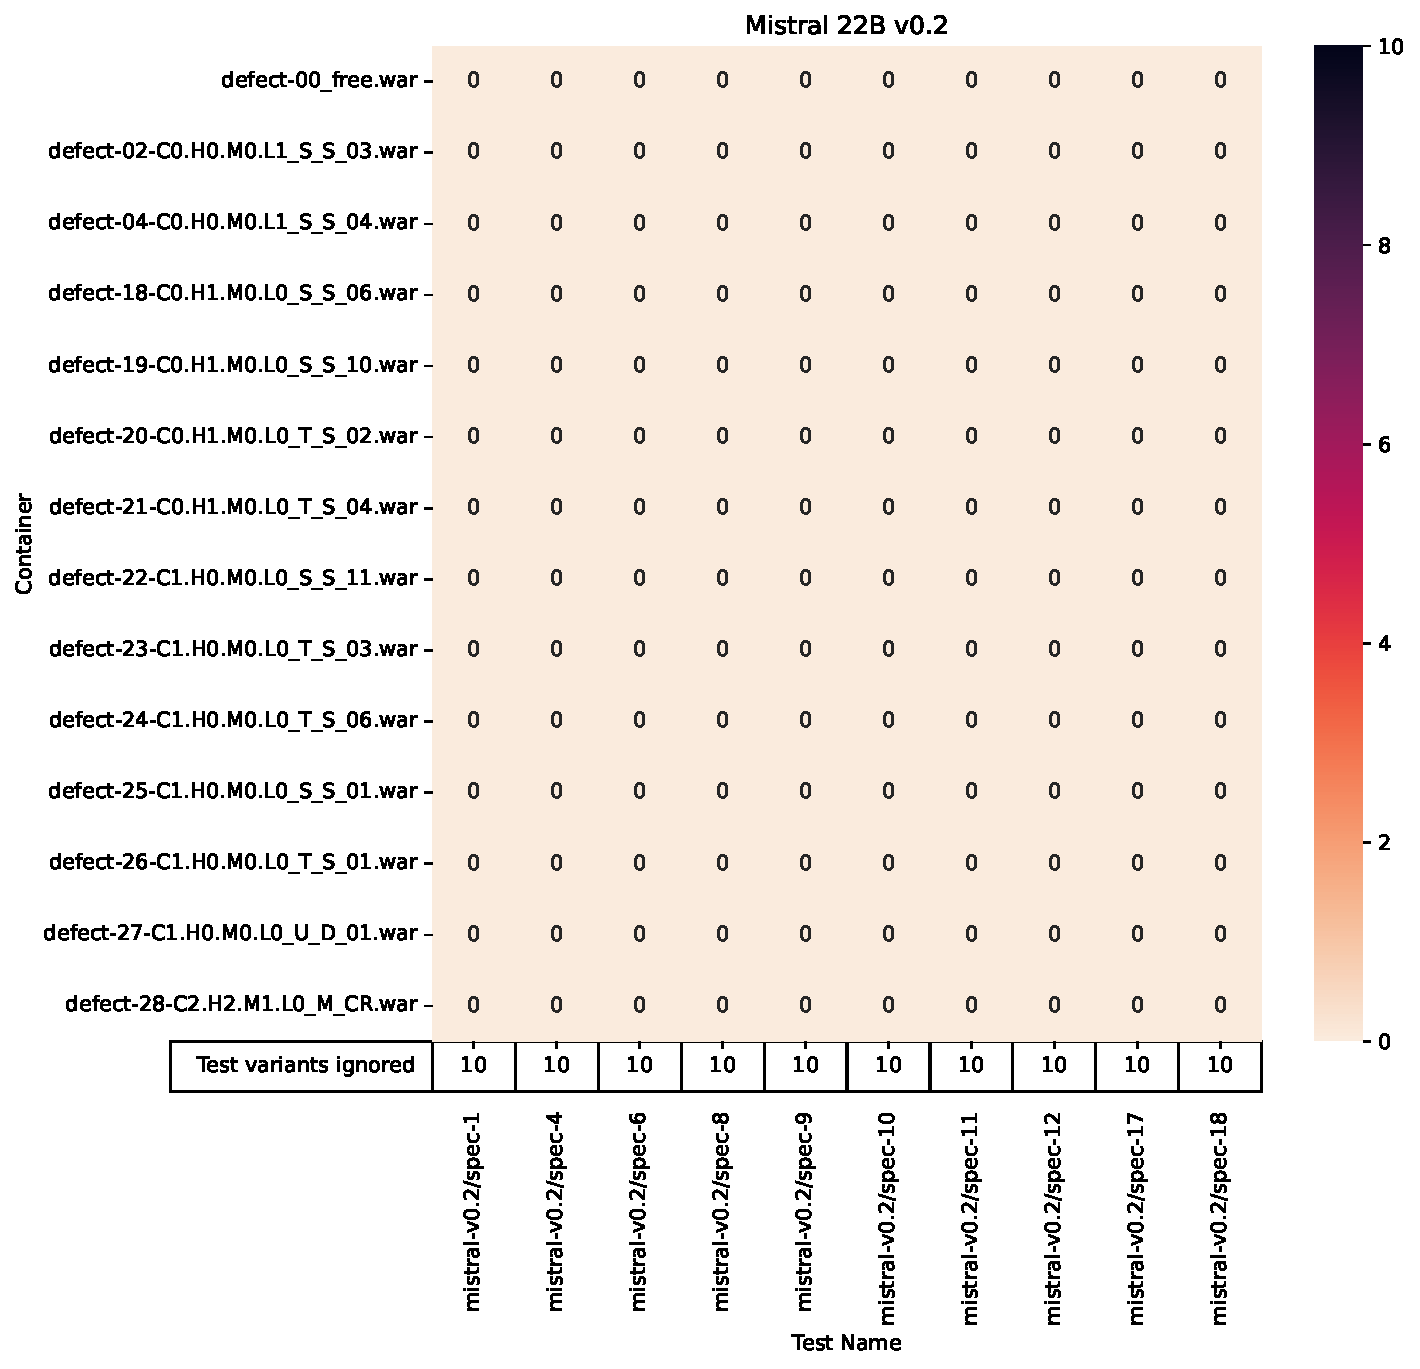
\includegraphics[width=\textwidth]{pic/mistral-v0.2-res.pdf}
            \caption{Výsledky pro model Mistral 7B v0.2}
            \label{fig:res:mistral-7b}
        \end{figure}

        \noindent Tato společnost nabízí i větší a proprietární model \textbf{Mistral Large}, který již byl schopen alespoň pro polovinu testových případů vygenerovat platný test. Konkrétně pro testy 4, 6, 10, 12, 17 a 18 nebyla vygenerována žádná z těchto variant (viz obr. \ref{fig:res:mistral-large}) a ve všech chybových testech se objevovali následující chyby:
        \begin{itemize}
            \item \emph{Neplatné přiřazení hodnoty XPath} - Stejný problém jako se objevoval např. v případě modelu Llama 3 (\ref{sec:res:meta}) nebo Claude 3 Opus (\ref{sec:res:anthropic}). Mezi argumentem a cestou chybí znak \verb|=| nebo \verb|:| a namísto nich se u cesty objevuje trojité \verb|/|.
            \item Neprovedení vstupu na \emph{přihlašovací obrazovku}. Tlačítko pro \emph{login} nebylo stisknuto a tedy prvky pro vyplnění přihlašovacího jména a hesla nebyly nalezeny.
            \item Využití neplatného \emph{XPath zápisu} (viz ukázka \ref{lst:mistral:wrong_xpath}). Zápis "xpath://*/[attr]" není v rámci XPath validní zápis a pro nalezení takovéhoto prvku by měl být využit zápis "xpath://*[attr]", tedy bez lomítka po \verb|*|.
            \item Nevyužití zástupného znaku pro klávesu \textit{Tab}. Tato klávesa může být využita pro přepnutí mezi textovým vstupem pro uživatelské jméno a heslo (není však nutná, protože RobotFramework vkládá hodnotu přímo do vstupního prvku). Protože model ke stisku klávesy využívá dnes zastaralé klíčové slovo \verb|Press Key| je v rámci něj potřeba využít pro tuto klávesu zástupný znak, jinak dojde k vypsání textové hodnoty \verb|TAB|, což se děje v některých vygenerovaných testech. Pokud by bylo využito klíčové slovo \verb|Press Keys|, k této chybě by nedošlo.
            \item Starý zápis pro \verb|FOR| smyčku (viz \ref{sec:res:meta}).
            \item Nesprávné \emph{klíčové slovo} pro kontrolu obsahu prvku. V ukázce \ref{lst:mistral:incorrect_keyword} lze vidět použití klíčového slova \verb|Page Should Contain Element|, které je platné, avšak podporuje jen první z argumentů a to cestu prvku, jehož existenci v rámci DOM stromu ověřuje. Model se však skrze něj snaží kontrolovat i textový obsah prvku. Takovouto funkci skutečně RobotFramework (resp. SeleniumLibrary) nabízí, ale pod klíčovým slovem \verb|Element Should Contain|.
            \item Vynechaná hlavička, obsahující import knihoven a základní nastavení testu. Viz výstup \verb|mistral-large/spec-17-5.robot|.
        \end{itemize}

        \begin{code}{robot}{Ukázka neplatného XPath zápisu. \label{lst:mistral:wrong_xpath}}
Input Text    xpath://*/[@id="loginPage.userNameInput"]    maroon
Input Password    xpath://*/[@id="loginPage.passwordInput"]    pass
Click Button    xpath://*/[@id="loginPage.loginFormSubmit"]
        \end{code}

        \begin{code}{robot}{Ukázka využití nesprávného klíčového slova. \label{lst:mistral:incorrect_keyword}}
Page Should Contain Element    xpath://*[@id="tea.listOfAllTeachers.table.teacherRow-0"]/td[3]    Numerical Methods
Page Should Contain Element    xpath://*[@id="tea.listOfAllTeachers.table.teacherRow-1"]/td[3]    Database Systems, Fundamentals of Computer Networks, Introduction to Algorithms, Mobile Applications, Web Programming
Page Should Not Contain Element    xpath://*[@id="tea.listOfAllTeachers.table.teacherRow-2"]/td[3]
Page Should Contain Element    xpath://*[@id="tea.listOfAllTeachers.table.teacherRow-3"]/td[3]    Computer System Engineering, Database Systems, Operating Systems, Programming Techniques
Page Should Contain Element    xpath://*[@id="tea.listOfAllTeachers.table.teacherRow-4"]/td[3]    Computation Structures
Page Should Contain Element    xpath://*[@id="tea.listOfAllTeachers.table.teacherRow-5"]/td[3]    Operating Systems, Programming in Java, Software Engineering, Software Quality Assurance
        \end{code}

        \noindent Z testů, které prošli kritérii pro ověření validity nedokázaly odhalit vložené chyby 3 z nich a to konkrétně pro test 1. Primárním problémem u variant testu 1, které nebyli schopné odhalit chybu, bylo nesprávné pořadí argumentu a zároveň použití nesprávného klíčového slova pro tuto kontrolu (viz ukázka \ref{lst:mistral:wrong_arg_order} na řádce 5), kde stejně jako bylo popsáno v předchozím odstavci by mělo být použito klíčové slovo \verb|Element Should Contain| a pořadí argumentů by mělo být obrácené.

        \begin{code}{robot}{Ukázka nesprávného pořadí argumentů. \label{lst:mistral:wrong_arg_order}}
Page Should Not Contain Element    id=header.link.login
Page Should Contain Element    id=header.title.userHome    Noah Brown
Page Should Contain Element    id=header.link.logout
Page Should Contain Element    css=#header.student-view-nav
Page Should Contain    Student's View    xpath://*[@id="stu.view.title"]
Page Should Contain Element    id=overview.personalInfoForm
        \end{code}

        \begin{figure}[H]
            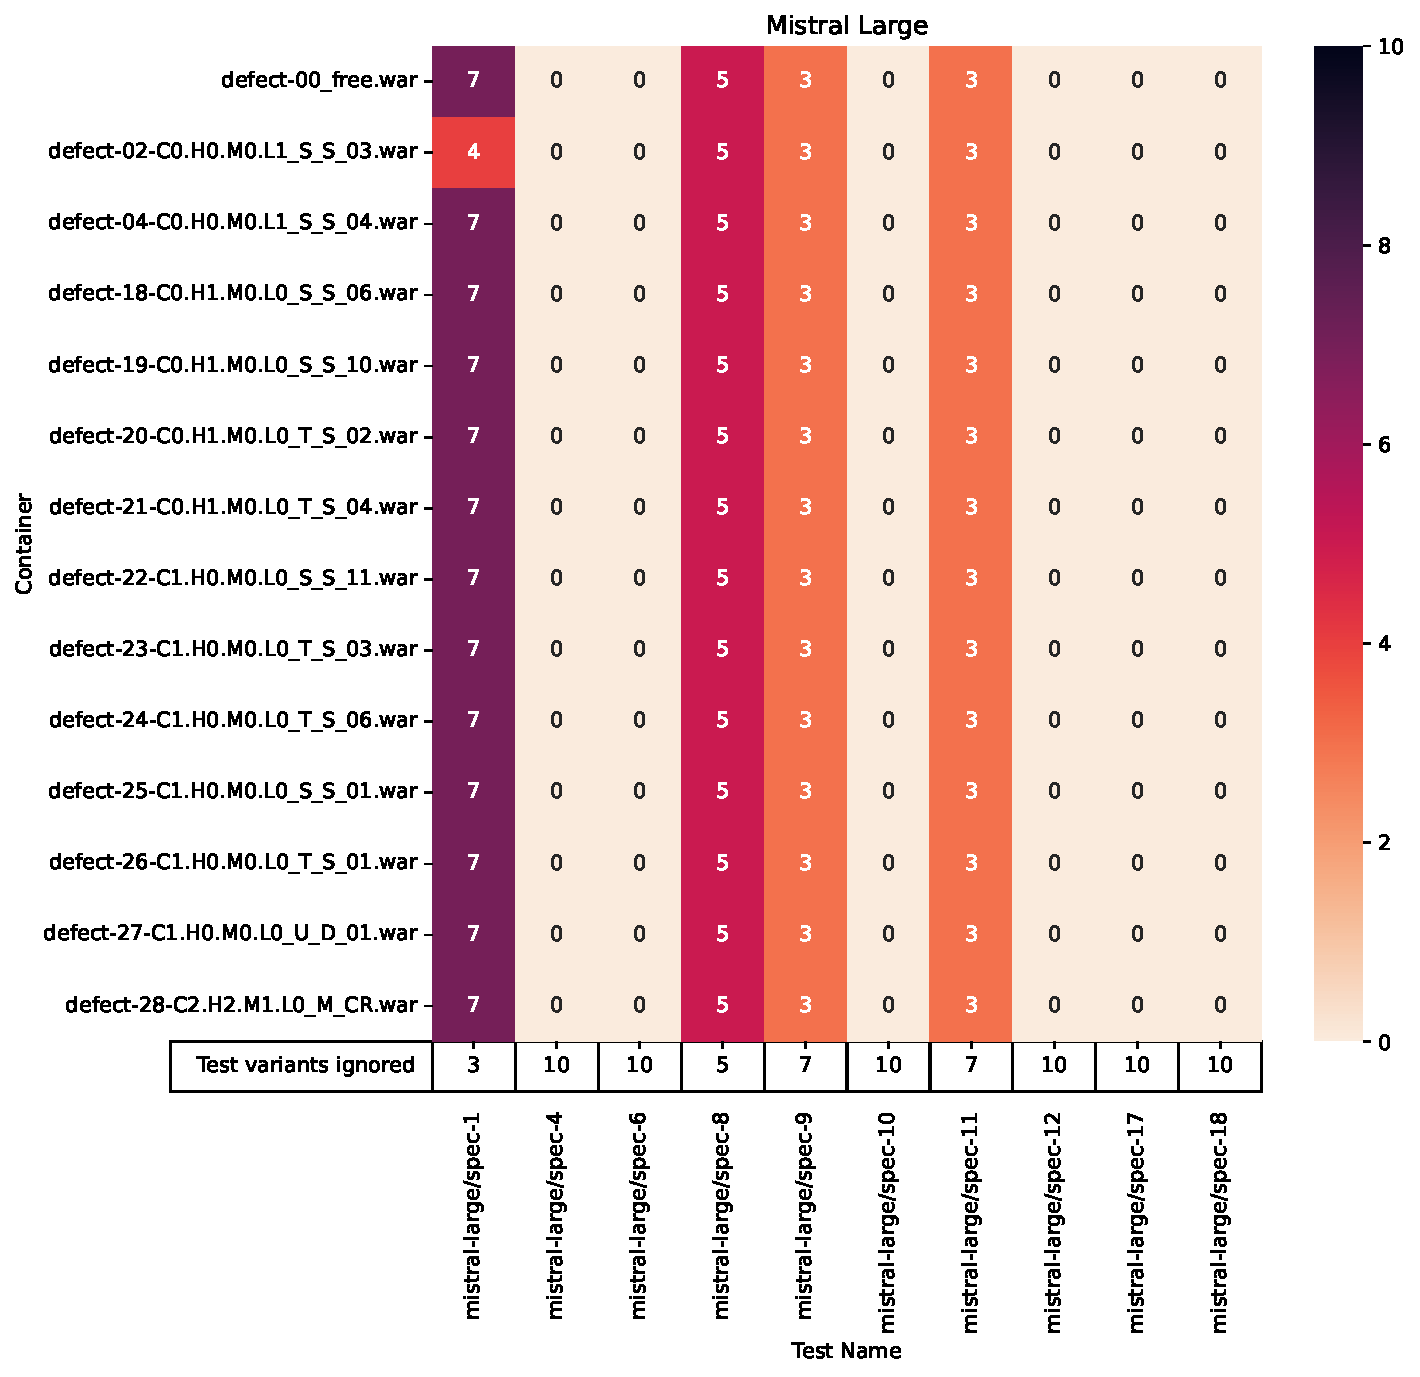
\includegraphics[width=\textwidth]{pic/mistral-large-results.pdf}
            \caption{Výsledky pro model Mistral Large.}
            \label{fig:res:mistral-large}
        \end{figure}

    \section{Kvalita výsledků}

    Protože pro \Acrshort{gui} testy nelze využít běžné metriky využívané v softwarovém testování \cite{COPPOLA2022107062}, bylo pro zhodnocení jejich kvality využita statistika úspěšnosti vygenerovaných tetů dle předpokladu pro jednotlivé modely a následně také došlo ke srovnání s testy psané člověkem, které jsou dostupné k projetu TbUIS v rámci samostatného repozitáře \footnote{\url{https://gitlab.kiv.zcu.cz/herout/tbuis-robotframework}}.

        \subsection{Úspěšnost LLM modelů v generování testů}

        Pro určení úspěšnosti a kvality jednotlivých modelů pro účely generování \Acrshort{gui} testů v Robot Framework zápisu jsme definovali následující metriky: 
        \begin{itemize}
            \item \textbf{Úspěšnost pro scénáře} - Pro kolik scénářů vygeneroval model alespoň jednu variantu testu, schopnou určit správné chování aplikace.
            \item \textbf{Celková úspěšnost případů} - Kolik ze všech 1400 spuštěných testů skončilo s očekávaným výsledkem pro nasazenou variantu aplikace při daném chodu (chybový stav se považuje za selhání).
            \item \textbf{Validita} - Kolik ze 100 vygenrovaných testových variant prošlo filtračním kritériem, popsaným v sekci \ref{sec:evaluation}. 
            \item \textbf{Úspěšnost z validních} - Kolik z validních testů bylo skutečně schopno odhalit vloženou chybu do systému. Poměr vůči předchozí metrice.
            \item \textbf{Celková úspěšnost testů} - Kolik ze 100 vygenerovaných testů bylo schopno odhalit jak běžné chování nasazené varinaty softwaru tak její defekt. Jedná se o poměr předchozí metriky vůči celkovému počtu vygenerovaných testů (100).
        \end{itemize}

        \begin{table}[H]
            \catcode`\-=12
            \begin{tabular}{|c|p{2cm}|p{2cm}|l|p{2cm}|p{2cm}|}
                \hline
                \textbf{Model} & \textbf{Úspěšnost pro \linebreak scénáře} & \textbf{Celková úspěšnost případů} & \textbf{Validita} & \textbf{Úspěšnost z validních} & \textbf{Celková úspěšnost testů} \\
                \hline
                \hline
                Claude 3 Opus & \textbf{100,00\%} & \textbf{43,71\%} & 47,00\% & \textbf{96,23\%} & \textbf{51,00\%} \\
                \hline
                GPT-4-Turbo   & 70,00\%  & 37,29\% & 39,00\% & 61,54\% & 46,00\% \\
                \hline
                Gemini 1.5 Pro & 90,00\% & 39,43\% & \textbf{48,00\%} & 87,50\% & 42,00\% \\
                \hline
                GPT-4         & 90,00\%  & 36,71\% & 39,00\% & 92,31\% & 36,00\% \\
                \hline
                Mistral Large & 40,00\%  & 17,79\% & 18,00\% & 83,33\% & 15,00\% \\
                \hline
                GPT-3.5 Turbo & 20,00\%  & 3,00\%  & 3,00\%  & 100,00\% & 3,00\% \\
                \hline
                CodeLlama     & 50,00\%  & 7,07\%  & 9,00\%  & 22,22\% & 2,00\% \\
                \hline
                Llama 3       & 10,00\%  & 2,00\%  & 2,00\%  & 100,00\% & 2,00\% \\
                \hline
                WizzardCoder  & 10,00\%  & 0,86\%  & 1,00\%  & 0,00\%  & 0,00\% \\
                \hline
                Mistral 7B    & 0,00\%   & 0,00\%  & 0,00\%  & 0,00\%  & 0,00\% \\
                \hline
            \end{tabular}
            \centering
            \caption{Výsledky metrik pro zhodnocení schopností modelů.}
            \label{tab:model_metrics}
        \end{table}

        Z výsledků (v tabulce \ref{tab:model_metrics}) lze usuzovat, že 

        %TODO Tabulka celkové úspěšnosti modelů

        \subsection{Srovnání s lidsky psanými testy}

        %TODO Tady asi jako zkusit code coverage a asi bych udělal srovnání s lidskými testy

    \section{Cena a časová náročnost generování}
    %TODO Je tohle dobré mít tady?

\chapter{Budoucí vylepšení}
    %TODO Jak snížit cenu - kratší prompty, komprese, atd.

\chapter{Závěr}
    %TODO Použitelné modely, co zlepšit

\appendix

    \chapter{Přiložené zdrojové kódy}

    \begin{code}{robot}{Korekntně vygenrovaný test dle specifikace 10 (soubor \uv{openai-gpt4/spec-10-3.robot}). \label{lst:gpt4:spec-10-3}}
*** Settings ***
Library           SeleniumLibrary
Suite Teardown    Close Browser

*** Test Cases ***
Teacher My Subjects And Exam Date Checks
    Open Browser    http://localhost:4680/tbuis/index.jsp    Chrome
    Set Window Size    1501    1104
    # Login Steps
    Click Element    xpath=//*[@id="header.link.login"]
    Sleep    1s
    Input Text    xpath=//*[@id="loginPage.userNameInput"]    strict
    Sleep    1s
    Input Text    xpath=//*[@id="loginPage.passwordInput"]    pass
    Sleep    1s
    Click Element    xpath=//*[@id="loginPage.loginFormSubmit"]
    Sleep    2s
    # My Subjects
    Click Element    xpath=//*[@id="tea.menu.mySubjects"]
    Sleep    2s
    Wait Until Element Is Not Visible    xpath=//button[@id!="tea.mySubjects.table.unregisterSubjectButton-0" and @value="Remove"]    10s
    Click Element    xpath=//*[@id="tea.mySubjects.table.unregisterSubjectButton-0"]
    Sleep    2s
    Page Should Contain Element    id=tea.mySubjects.successAlert
    # My Exam Dates
    Click Element    xpath=//*[@id="tea.menu.myExamDates"]
    Sleep    2s
    Element Should Not Be Visible    xpath=//th[contains(., "Operating Systems")]
    # New Exam Dates
    Click Element    xpath=//*[@id="tea.menu.newExamDates"]
    Sleep    2s
    Element Should Not Be Visible    xpath=//option[contains(., "Operating Systems")]
    # Set Evaluation
    Click Element    xpath=//*[@id="tea.menu.setEvaluation"]
    Sleep    2s
    Element Should Not Be Visible    xpath=//option[contains(., "Operating Systems")]
    # Evaluation Table
    Click Element    xpath=//*[@id="tea.menu.evaluationTable"]
    Sleep    2s
    Element Should Not Be Visible    xpath=//option[contains(., "Operating Systems")]
    # Other's Subjects
    Click Element    xpath=//*[@id="tea.menu.otherSubjects"]
    Sleep    2s
    Page Should Contain Element    xpath=//td[contains(., "Operating Systems")]
    # List of All Teachers
    Click Element    xpath=//*[@id="tea.menu.listOfAllTeachers"]
    Sleep    2s
    Element Should Not Contain    xpath=//*[@id="tea.listOfAllTeachers.table.teacherRow-5"]    "Operating Systems"
    Close Browser

Student Other Subjects Check
    Open Browser    http://localhost:4680/tbuis/index.jsp    Chrome
    Set Window Size    1501    1104
    # Login Steps
    Click Element    xpath=//*[@id="header.link.login"]
    Sleep    1s
    Input Text    xpath=//*[@id="loginPage.userNameInput"]    orange
    Sleep    1s
    Input Text    xpath=//*[@id="loginPage.passwordInput"]    pass
    Sleep    1s
    Click Element    xpath=//*[@id="loginPage.loginFormSubmit"]
    Sleep    2s
    # Other Subjects
    Click Element    xpath=//*[@id="stu.menu.otherSubjects"]
    Sleep    2s
    ${is_present}=    Run Keyword And Return Status    Element Should Not Contain    xpath=//tr[contains(., "Operating Systems")]    "Peter Strict"
    Should Be True    ${is_present}
    Close Browser\end{code}

    \begin{code}{robot}{Ručně psaný test pro specifikaci 10. \label{lst:acc:spec-10-root}}
*** Settings ***

Resource          ../../baseKeywords.robot
Resource          ../../keywords/scenarios/subjects/cancel/teaching.robot

Variables         ../data/teacher/UC10_CancellationSubject.yaml

Suite Setup       Prepare Suite without DB restore
Test Setup        Prepare Test with DB restore
Suite Teardown    End Test

*** Test Cases ***

TC.10.01 Teacher Cancel Teaching Of Subject
    [Template]          Cancel Subject Teaching Success
    [Tags]              UC.10  HappyDay  MAJOR
    [Documentation]     In this test case teacher cancel teaching of subject when all preconditions are fullfilled.
    ...
    FOR    ${params}    IN    @{SuccessCancellations}
       @{params}
    END

TC.10.02 Teacher Cancel Teaching Of Subject Fails - Some Students Enrolled
    [Template]          Cancel Subject Teaching Failiture
    [Tags]              UC.10  MINOR
    [Documentation]     In this test case teacher tries cancel subject where some students are enrolled.
    ...
    FOR    ${params}    IN    @{SomeStudentsEnrolled}
       @{params}
    END

TC.10.03 Teacher Cancel Teaching Of Subject Fails - Teacher does not teach this subject
    [Template]          Cancel Subject Teaching Not Found
    [Tags]              UC.10  MINOR
    [Documentation]     In this test case teacher try leave subject which is not teached by.
    ...
    FOR    ${params}    IN    @{WrongSubject}
       @{params}
    END\end{code}

\appendix

% _____________________________________________________________________________
%
%
%        BACK MATTER (BIBLIOGRAPHY, LISTS, ...)
%
% _____________________________________________________________________________
%
\backmatter
\printbibliography
\listoffigures
\listoftables
\listoflistings
% _____________________________________________________________________________
%
%		BACK COVER
% _____________________________________________________________________________
%
%\setbackpagepic{img/fav} % <== an example of one possible option (read this manual)
%\setqrcodebaseurl{https://mycloud.org/show=pdf&docid=} % <== another example
%\setbackpageqrcode{54321} % <== and one more (uncomment the one that makes sense for you)
\setbackpageqrcode
\backpage
\end{document}
